%\documentclass[12pt]{scrreprt}
\documentclass[12pt]{report} 

% language may be romanian or english (default is english)
% type may be bachelor or master (default is bachelor)
\usepackage[language=english, type=bachelor]{style}

%\geometry{a4paper,top=2.5cm,left=3cm,right=2.5cm,bottom=2.5cm}
%in style
%controlling the appearance of your headers and footers
\usepackage{fancyhdr}
\pagestyle{fancy}
\lhead{}
\chead{}
\renewcommand{\headrulewidth}{0.2pt}
\renewcommand{\footrulewidth}{0.2pt}

\usepackage{amsmath}
\usepackage{amssymb}
\usepackage{array}
\usepackage{booktabs}
\usepackage{tabularx}
\newcolumntype{Y}{>{\raggedright\arraybackslash}X}
\usepackage{longtable}
\usepackage{ltablex}
\keepXColumns
\usepackage{float}
\usepackage{graphicx}
\usepackage{tikz}
\usetikzlibrary{positioning,arrows.meta,fit,shapes.geometric,shapes.multipart,backgrounds}
\usepackage{pgfplots}
\pgfplotsset{compat=1.18}
\usepgfplotslibrary{groupplots}

\usepackage{xcolor}
\usepackage{listings}

\hypersetup{
    colorlinks=true,
    linkcolor=blue,
    citecolor=blue,
    urlcolor=blue,
    filecolor=blue,
    pdfborder={0 0 0}
}

\makeatletter
\renewcommand\paragraph{\@startsection{paragraph}{4}{\z@}%
  {2.5ex \@plus 1ex \@minus .2ex}%
  {1ex \@plus .2ex}%
  {\normalfont\normalsize\bfseries}}
\makeatother

\definecolor{lstKeyword}{RGB}{0, 51, 178}
\definecolor{lstString}{RGB}{163, 21, 21}
\definecolor{lstComment}{RGB}{0, 128, 0}
\definecolor{lstType}{RGB}{43, 145, 175}
\definecolor{lstBg}{RGB}{248, 248, 248}
\definecolor{lstFrame}{RGB}{210, 210, 210}

\lstset{
    basicstyle=\ttfamily\footnotesize,
    breaklines=true,
    frame=single,
    rulecolor=\color{lstFrame},
    backgroundcolor=\color{lstBg},
    showstringspaces=false,
    keywordstyle=\bfseries\color{lstKeyword},
    stringstyle=\color{lstString},
    commentstyle=\itshape\color{lstComment},
    emphstyle=\color{lstType},
    columns=fullflexible,
    captionpos=b
}

\lstdefinestyle{csharp}{
    language={[Sharp]C},
    morekeywords={var, async, await, Task, IReadOnlyList, CancellationToken},
    emph={ImageGenerationResult, IImageProvider},
    emphstyle=\color{lstType}
}

\begin{document}

% --- PRIMA PAGINĂ (Păstrată) ---
\specialization{COMPUTER SCIENCE IN ENGLISH}
\title{Automating Marketing Assets through Generative RAG and Contextual Recommendation}
\author{Borodi Bogdan-Vasile}
\supervisor{Lect. Horea-Bogdan Mure\c{s}an}

\maketitle

% --- SECȚIUNEA ELIMINATĂ ERA AICI ---

\newpage
\thispagestyle{empty}
\mbox{}
\newpage
\pagenumbering{roman} 

\cleardoublepage
ABSTRACT
\vspace{0.5cm}	
\hrule
\vspace{0.5cm}	

Small and independent retailers need professional digital marketing materials but lack the time, budget and design expertise that larger competitors take for granted. This thesis presents a cross-platform application that automates the creation of marketing assets, such as promotional announcements, product catalogues and brand wallpapers, directly from a retailer's own product photographs and shop information, so that visual campaigns can be produced in seconds from a phone or a desktop browser and exported in print-ready quality when a physical poster is needed.

\textit{Chapter 1} motivates the work and states its objectives. \textit{Chapter 2} introduces the theoretical foundations: image-generating models, prompt design, retrieval-augmented generation and learned visual similarity. \textit{Chapter 3} describes the system architecture and its deployment on Microsoft Azure. \textit{Chapter 4} presents three technical contributions: a recommendation engine that pairs retrieval-augmented context with a fine-tuned writer model to produce fresh marketing themes from a curated promotional playbook, a hybrid generation technique that preserves the retailer's product photograph while the model designs the surrounding scene, and a print pipeline that upscales finished assets with a learned super-resolution model so they remain sharp from A6 to A3. \textit{Chapter 5} reports the platform's results, sample generated assets, the layered automated test suite and an offline evaluation harness that compares candidate writer models on a frozen reference set.

The main contribution is the design and implementation of an end-to-end system that brings generative AI into the daily workflow of non-technical retailers. The platform combines prompt strategies tailored to each asset family, a retrieval-grounded daily recommender driven by a fine-tuned writer model, a hybrid generative-deterministic pipeline that keeps the retailer's actual products faithful, and a learned super-resolution stage that lifts finished assets to print quality. Experimentation showed that purely generative approaches are insufficient for marketing content that must stay truthful to a real product, while a small amount of deterministic compositing applied after generation removes this limitation at a manageable cost.

The thesis offers original insights into the trade-offs between fully generative pipelines and hybrid generative-deterministic ones, into the value of grounding daily marketing suggestions in real-world contextual signals, and into evidence-based model selection for the writer stage of a retrieval-augmented marketing assistant.

\tableofcontents

\newpage
\pagenumbering{arabic}

% Chapter inputs are commented out until each chapter file is authored.
% Uncomment each line once chapters/<name>.tex exists, otherwise LaTeX aborts and produces no PDF.
\chapter{Introduction}
\label{chap:introduction}

\section{Context}

Small and independent retailers, such as a local craft shop or a neighbourhood restaurant, face a structural disadvantage when it comes to marketing. Larger competitors employ in-house design teams and external creative agencies that produce a steady stream of polished promotional material throughout the year. Independent shops, by contrast, rarely have the time or the expertise to produce the kind of professional visual content that today's customers have come to expect on social media and in physical storefronts. The result is a visible quality gap between large brands and the local businesses that compete with them, and this gap continues to widen as larger competitors invest aggressively in digital marketing.

In the last few years, generative artificial intelligence has begun to close part of this gap. Modern image-generating models can produce near-photographic visuals from a short text prompt, and conversational language models can draft promotional copy on demand. In principle, these tools should be transformative for small retailers; in practice, however, the leap from a general-purpose model to a polished, brand-consistent advertisement is far from trivial. Models often produce renderings that look good in isolation but misrepresent the product itself, struggle to reproduce a retailer's exact branding (a particular logo or a chosen colour palette, for instance), and require careful prompting that most non-technical users are not equipped to perform. They also do not, on their own, decide when a campaign should be run, or what theme would resonate with a particular local audience on a particular day.

The platform presented in this thesis was developed against this backdrop. It treats marketing automation as more than a single image-generation step. It records the retailer's brand profile alongside a library of their products, watches a small set of real-world contextual signals (current weather, upcoming holidays, recent news) and uses them to suggest daily marketing ideas. When the retailer likes an idea, the platform can then turn it into a finished asset to publish. The client side runs on both desktop web browsers and mobile devices from a single React Native codebase, and the service is hosted on the Microsoft Azure cloud as a regular production deployment rather than as a controlled experiment.

\section{Objectives}
\label{sec:objectives}

Concretely, this thesis pursues the following objectives:

\begin{itemize}
    \item To design and implement a cross-platform application that automates the production of marketing assets directly from a retailer's product photographs and shop information.
    \item To enable retailers to assemble their product library with minimal manual effort, either by uploading their own photographs and removing the background automatically through an AI model, or by searching a curated reference database by visual similarity to a sample photo or by name.
    \item To develop a recommendation engine that suggests fresh marketing ideas on a daily basis, grounded in real-world contextual signals such as the weather, upcoming holidays and recent news, so that the platform is useful as an everyday tool rather than a one-off generator.
    \item To investigate and implement a hybrid generation strategy in which a generative model designs the surrounding scene while the retailer's actual product photograph is preserved through deterministic post-processing, addressing a well-known limitation of current models in faithfully reproducing specific real-world objects. The same pipeline is then extended with a high-resolution rendering path that produces print-ready posters for display in the shop itself.
    \item To package the resulting platform as a cloud service deployed on Microsoft Azure, to demonstrate that the proposed approach is viable beyond a controlled experimental setting.
\end{itemize}

\section{Thesis Structure}

The remainder of this thesis is organised as follows. Chapter 2 reviews the theoretical foundations on which the system is built: modern image-generating models, prompt engineering, retrieval-augmented generation, and techniques for measuring visual similarity between images. Chapter 3 is devoted to the overall architecture of the platform and to its deployment on the Microsoft Azure cloud. The implementation is then presented in Chapter 4, with a particular focus on the recommendation engine and the hybrid generation technique that together constitute the main technical contributions of this work. Chapter 5 covers the testing strategy, including both the automated suites for architectural correctness and the offline evaluation protocol applied to the language-model output. Chapter 6 closes the thesis with a summary of the contributions and a number of directions for future work.

During the preparation of this work the author used ChatGPT to improve the language and readability of the thesis. After using ChatGPT, I reviewed and edited the content as needed. All experimental results, model training, system design, evaluation, and scientific conclusions are entirely my own work. I take full responsibility for the accuracy and integrity of the final document.

\chapter{Theoretical Background}
\label{chap:background}

The platform proposed in this thesis sits at the intersection of several research areas: image generation by neural networks, the practice of guiding such networks through carefully designed prompts, retrieval-augmented generation as a means of grounding large language models in external knowledge, and the use of learned visual representations to compare images. The aim of this chapter is to introduce the concepts and vocabulary on which the rest of the thesis depends, so that the architectural choices in \textit{Chapter 3} and the implementation details in \textit{Chapter 4} can be discussed with the appropriate technical precision. No attempt is made at exhaustive coverage; the focus is firmly on those ideas that recur in subsequent chapters.

\section{Generative Models for Image Synthesis}
\label{sec:generative-models}

The first technical pillar of the proposed application is the synthesis of photorealistic marketing imagery from a textual description and, in some cases, from one or more reference photographs supplied by the retailer. This section reviews how generative models have come to make such synthesis possible, with particular attention to the diffusion-based approach that underpins most of today's high-quality systems and to the more recent class of multimodal foundation models that can accept both text and images as input.

\subsection{The generative modelling problem}

Image generation is the task of drawing samples from a probability distribution over images. A generative model attempts to approximate the unknown data distribution \(p_{\text{data}}(x)\) of natural images using a parametric distribution \(p_\theta(x)\), so that new samples drawn from \(p_\theta\) are indistinguishable from real photographs to a human observer. In modern conditional generation, the distribution is further conditioned on a textual description \(c\), and the task becomes that of sampling from \(p_\theta(x \mid c)\).

Generative adversarial networks (GANs) \cite{goodfellow2014gan} and variational autoencoders (VAEs) \cite{kingma2014vae} dominated the field before the diffusion era, but each suffers well-known drawbacks (training instability and mode collapse for GANs, blurred outputs for VAEs) that limit their use for the kind of photorealistic synthesis required here. Table~\ref{tab:generative-paradigms} summarises the two paradigms that dominate the present landscape and which this thesis builds on.

\begin{table}[ht]
\centering
\caption{Generative-model paradigms relevant to this thesis.}
\label{tab:generative-paradigms}
\small
\renewcommand{\arraystretch}{1.3}
\begin{tabular}{@{}>{\raggedright\arraybackslash}p{2.7cm}
                  >{\raggedright\arraybackslash}p{2.4cm}
                  >{\raggedright\arraybackslash}p{1.6cm}
                  >{\raggedright\arraybackslash}p{2.2cm}
                  >{\raggedright\arraybackslash}p{2.6cm}@{}}
\toprule
\textbf{Paradigm} & \textbf{Training objective} & \textbf{Sampling cost} & \textbf{Conditioning} & \textbf{Suitability} \\
\midrule
Diffusion \cite{ho2020ddpm,rombach2022ldm} & Denoising score matching & High (many steps) & Strong via guidance & Backbone of most modern systems \\
\addlinespace[4pt]
Multimodal LLM with image output & LLM front-end over diffusion submodel & Moderate & Native (text and image) & Used by the platform \\
\bottomrule
\end{tabular}
\end{table}

\subsection{Diffusion models}

Denoising diffusion probabilistic models \cite{ho2020ddpm} have, since 2020, become the dominant approach to high-fidelity image synthesis. The intuition is appealingly simple. A \emph{forward process} progressively corrupts a clean image \(x_0\) by adding small amounts of Gaussian noise over \(T\) time-steps, producing a sequence \(x_0, x_1, \dots, x_T\) in which \(x_T\) is essentially pure noise. The forward step is

\begin{equation}
q(x_t \mid x_{t-1}) = \mathcal{N}\big(x_t;\; \sqrt{1 - \beta_t}\, x_{t-1},\; \beta_t \mathbf{I}\big),
\label{eq:diffusion-forward}
\end{equation}

where \(\{\beta_t\}_{t=1}^{T}\) is a fixed variance schedule. A neural network, typically a U-Net, is then trained to invert each step of this process: given a noisy \(x_t\), it predicts the noise that was added, which is equivalent to predicting a slightly less noisy \(x_{t-1}\). At inference time, sampling proceeds in reverse, starting from random Gaussian noise and gradually denoising it into a coherent image, as illustrated schematically in Figure~\ref{fig:diffusion}.

Conditional generation is most commonly achieved through \emph{classifier-free guidance}, in which the same network is trained both with and without the textual condition \(c\), and at sampling time the predicted noise is extrapolated away from the unconditional prediction and towards the conditional one. This yields strong text adherence at the cost of some sample diversity. Latent diffusion models \cite{rombach2022ldm}, of which Stable Diffusion is the best known instance, perform the entire diffusion process in the compressed latent space of a pretrained autoencoder rather than at the pixel level, which dramatically reduces the computational cost of training and sampling. The text condition itself is supplied by a separate language encoder, often a transformer \cite{vaswani2017attention}, whose output embeddings are injected into the U-Net through cross-attention layers.

\begin{figure}[ht]
\centering
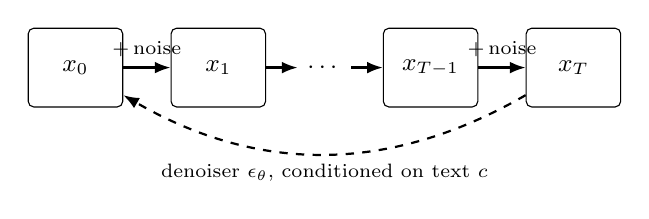
\begin{tikzpicture}[
    node distance=10mm and 6mm,
    every node/.style={font=\small},
    box/.style={draw, rounded corners=2pt, minimum width=12mm, minimum height=10mm, align=center},
    arr/.style={-{Latex[length=2mm]}, thick}
]
\node[box] (x0) {$x_0$};
\node[box, right=of x0] (x1) {$x_1$};
\node[right=4mm of x1] (dots) {$\cdots$};
\node[box, right=4mm of dots] (xt1) {$x_{T-1}$};
\node[box, right=of xt1] (xt) {$x_T$};

\draw[arr] (x0) -- node[above, font=\scriptsize] {$+\,\text{noise}$} (x1);
\draw[arr] (x1) -- (dots);
\draw[arr] (dots) -- (xt1);
\draw[arr] (xt1) -- node[above, font=\scriptsize] {$+\,\text{noise}$} (xt);

\draw[arr, dashed, bend left=30] (xt) to node[below, font=\scriptsize] {denoiser $\epsilon_\theta$, conditioned on text $c$} (x0);
\end{tikzpicture}
\caption{The forward and reverse processes of a diffusion model. The forward chain (solid) gradually adds noise to a clean image until it becomes pure Gaussian noise. A learned denoiser, conditioned on a text prompt~\(c\), reverses the chain (dashed) at sampling time.}
\label{fig:diffusion}
\end{figure}

\subsection{Multimodal foundation models and their limitations}

A more recent line of work places a multimodal large language model in front of the image generator. Familiar examples are ChatGPT, which routes image-generation requests to DALL-E, and Gemini, which calls one of Google's image submodels (most recently the Nano-Banana family). The user supplies text and reference images in a single prompt; the front-end model encodes both modalities into a shared embedding space (Section~\ref{sec:rag}) and orchestrates an underlying, usually diffusion-based, submodel that produces the pixels. Through attention over the supplied references, such systems can be instructed to preserve specific elements (a logo, a product, a colour palette) and typically respect those instructions, although the result is rarely a pixel-perfect copy. The diffusion techniques described above are therefore not superseded but wrapped inside a multimodal interface that can express tasks like ``redesign this poster while keeping the logo intact'' in a single call.

The proposed application relies on a multimodal model of this latter kind. A single call can ingest the shop's logo, the product photographs, and the textual description of the desired scene, removing the need for a separate input-side compositing step; and the model's image-to-image capability is a prerequisite for the hybrid pipeline of Section~\ref{sec:hybrid}, where the generator produces a scene around designated placeholder regions rather than a finished advertisement.

For all their fluency, modern image generators have well-documented weaknesses. Three are directly relevant to this thesis. First, \emph{identity preservation} of specific real-world objects is brittle: even with a clean reference photograph, the generator tends to alter colour, texture, label, or shape in commercially unacceptable ways. Second, photorealistic \emph{text rendering}, although greatly improved in the latest model generations, remains unreliable for non-trivial strings such as price tags or longer slogans. Third, \emph{brand fidelity} is hard to enforce through prompting alone: a precise hex colour or a particular typeface is rarely reproduced exactly. Section~\ref{sec:hybrid} addresses these limitations through a hybrid pipeline that reduces the model's responsibility to producing a background scene with reserved regions, leaving product placement and text rendering to deterministic post-processing.

\section{Prompt Engineering}
\label{sec:prompt-engineering}

The output quality of modern generative models depends sharply on prompt phrasing. \emph{Prompt engineering} is the body of empirically discovered patterns for coaxing reliable output from models otherwise treated as black boxes; this section covers the patterns used by the proposed application.

\subsection{Anatomy of a prompt}

A well-formed prompt for a modern generative model can be decomposed into several distinguishable parts: a \emph{role} or \emph{persona} that establishes the perspective from which the model should reason; a \emph{context} block supplying domain-specific facts; an \emph{instruction} stating what the model is to produce; a set of \emph{constraints} on the output's form and content; and, optionally, an \emph{output format} specification when downstream parsing is required. Figure~\ref{fig:prompt-anatomy} illustrates the layout used by the catalogue-generation prompts in the proposed system.

\begin{figure}[ht]
\centering
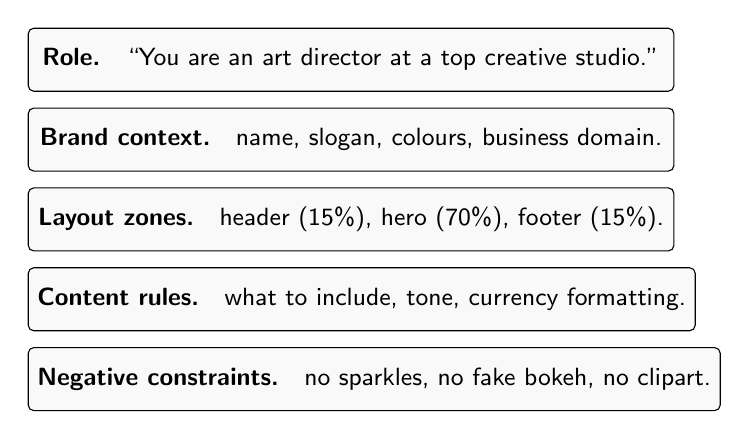
\begin{tikzpicture}[
    every node/.style={font=\small\sffamily},
    block/.style={draw, rounded corners=2pt, minimum width=82mm, minimum height=8mm, anchor=west, fill=gray!5},
    label/.style={font=\scriptsize\itshape, gray}
]
\node[block] (role) at (0,0)         {\textbf{Role.}\;\; ``You are an art director at a top creative studio.''};
\node[block, below=2mm of role.south west, anchor=north west] (ctx) {\textbf{Brand context.}\;\; name, slogan, colours, business domain.};
\node[block, below=2mm of ctx.south west, anchor=north west] (layout) {\textbf{Layout zones.}\;\; header (15\%), hero (70\%), footer (15\%).};
\node[block, below=2mm of layout.south west, anchor=north west] (rules) {\textbf{Content rules.}\;\; what to include, tone, currency formatting.};
\node[block, below=2mm of rules.south west, anchor=north west] (neg) {\textbf{Negative constraints.}\;\; no sparkles, no fake bokeh, no clipart.};
\end{tikzpicture}
\caption{Anatomy of a structured prompt for image generation.}
\label{fig:prompt-anatomy}
\end{figure}

\subsection{Prompting patterns used by the platform}

Of the three standard prompting styles (zero-shot, few-shot, and chain-of-thought \cite{wei2022cot}), the proposed application uses zero-shot for image generation, where in-context examples would themselves be images and inflate the token budget, and chain-of-thought in the recommendation engine of Section~\ref{sec:rag}, where a chained sequence of language-model calls reasons about marketing themes before drafting them. Two further techniques recur throughout the platform: layout-aware prompting and multimodal prompting.

\paragraph{Structured and layout-aware prompting.}
When the desired output has a non-trivial spatial structure, the prompt itself can declare that structure explicitly. In the proposed application, wallpaper prompts allocate the canvas into a header band, a hero area, and a footer band, each with a specific percentage of the vertical space and a specific responsibility (the hero band carries the product, the footer the contact information, and so on). Catalogue prompts go further still, declaring placeholder regions in which the actual product photographs will subsequently be pasted by a deterministic compositor. Such layout-aware prompting reduces the model's task from ``design an entire advertisement'' to ``design a scene that respects this layout'', which is markedly easier and considerably more controllable.

\paragraph{Multimodal prompting.}
Multimodal prompting refers to the practice of including reference images, alongside textual instructions, inside a single prompt. In the proposed application this is used routinely: the brand logo is supplied as a reference image so that the model can place it without re-inventing it, and product photographs are supplied so that the model can lay out a scene around them. This is qualitatively different from a text-only prompt asking for ``a coffee shop logo on a wooden table'': the model is shown the actual logo, not merely told that one exists.

\section{Retrieval-Augmented Generation}
\label{sec:rag}

Large language models are remarkably fluent, but they are also famously unreliable on facts that lie outside their training distribution: recent events, niche technical details, or anything that is private to a particular user or organisation. \emph{Retrieval-augmented generation} (RAG) is a now-standard architectural response to this limitation \cite{lewis2020rag}: instead of asking a model to answer from its parameters alone, the system first retrieves relevant external information from a separate store and includes it inside the prompt, so that the model can ground its output in that information rather than relying on memorised knowledge.

\subsection{Motivation: grounding language models in external knowledge}

Retrieval augmentation promotes external storage to a first-class element of the inference pipeline, sidestepping three known weaknesses of pure language models: a bounded context window, a tendency to hallucinate verifiable facts, and the high cost of fine-tuning relative to updating a retrieval index.

The daily recommendation engine of \textit{Chapter 4} uses two retrieval passes: one over the user's recently generated ideas to discourage repetition, and one over a curated knowledge base of promotional tactics organised by business domain so that suggestions are anchored in patterns known to work for shops of that type.

\subsection{Vector embeddings and approximate nearest-neighbour search}

The retrieval step in a RAG pipeline does not, in general, search for literal keyword matches; it searches for semantic ones. The standard mechanism is to map each indexed item (a paragraph, a product description, an image) into a fixed-length vector in \(\mathbb{R}^d\), in such a way that semantically similar items are close together in vector space. Such mappings are known as \emph{embeddings}, and they are produced by neural encoders trained either on language data alone or jointly on language and vision (Section~\ref{sec:visual-similarity}).

This dense, embedding-based approach contrasts with classical sparse retrieval methods such as TF--IDF and BM25, which represent documents by very high-dimensional sparse vectors of term frequencies. Sparse methods remain competitive when the user query and the indexed text share vocabulary, but they fail in the common case where two passages express the same idea using different words, or where the query is an image rather than a text. Dense embeddings handle both cases naturally.

Once items have been embedded, retrieval reduces to finding the \(k\) nearest neighbours of a query vector under some distance function, typically cosine distance for normalised embeddings. Exact search through every indexed vector is linear in the size of the index and quickly becomes infeasible for collections beyond a few hundred thousand items. The standard remedy is to use an \emph{approximate nearest-neighbour} (ANN) index, which trades a small amount of recall for a substantial speed-up.

The Hierarchical Navigable Small World (HNSW) algorithm \cite{malkov2018hnsw} is among the most widely used such indexes and is the one chosen by the proposed application. HNSW organises the vectors into a multi-layer graph with small-world properties: search descends from a sparse top layer through progressively denser ones, refining the nearest-neighbour estimate at each level. The proposed application uses the common defaults \(M = 16\) (bidirectional links per node) and \textit{ef\_construction}\,\(= 64\), which strike a reasonable balance between index size, build time, and recall for collections in the tens of thousands.

\subsection{The retrieve--augment--generate pipeline}

Conceptually, a RAG pipeline operates in three steps, illustrated in Figure~\ref{fig:rag}: \emph{retrieve} the top-\(k\) items most relevant to the user's query, \emph{augment} the prompt by including those items as additional context, and \emph{generate} the final answer by running the augmented prompt through the language model. The retrieval step is responsible for relevance; the augmentation step for fitting the retrieved material into the model's context window; and the generation step for producing fluent, well-formed output that respects the retrieved evidence.

\begin{figure}[ht]
\centering
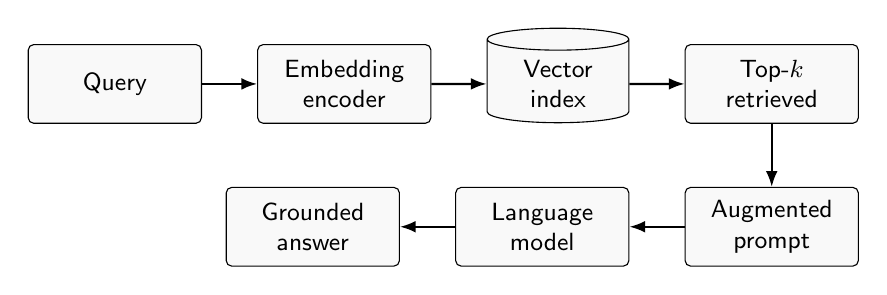
\begin{tikzpicture}[
    node distance=8mm and 7mm,
    every node/.style={font=\small\sffamily},
    box/.style={draw, rounded corners=2pt, minimum width=22mm, minimum height=10mm, align=center, fill=gray!5},
    store/.style={draw, cylinder, shape border rotate=90, aspect=0.25, minimum width=18mm, minimum height=12mm, align=center, fill=gray!5},
    arr/.style={-{Latex[length=2mm]}, thick}
]
\node[box] (q) {Query};
\node[box, right=of q] (emb) {Embedding\\encoder};
\node[store, right=of emb] (idx) {Vector\\index};
\node[box, right=of idx] (top) {Top-\(k\)\\retrieved};
\node[box, below=8mm of top] (prompt) {Augmented\\prompt};
\node[box, left=of prompt] (llm) {Language\\model};
\node[box, left=of llm] (ans) {Grounded\\answer};

\draw[arr] (q) -- (emb);
\draw[arr] (emb) -- (idx);
\draw[arr] (idx) -- (top);
\draw[arr] (top) -- (prompt);
\draw[arr] (prompt) -- (llm);
\draw[arr] (llm) -- (ans);
\end{tikzpicture}
\caption{The retrieve--augment--generate pipeline. A query is embedded, the index returns the top-\(k\) most similar entries, those entries are spliced into a prompt, and the language model produces an answer grounded in the retrieved material.}
\label{fig:rag}
\end{figure}

\subsection{Structured outputs and multi-agent orchestration}

A practical RAG system rarely consists of a single language-model call. Decomposing a task into a chain of smaller, focused prompts with JSON-mode constrained decoding produces more reliable output than one opaque call and turns the pipeline into a controllable, observable structure that can be debugged component by component. The recommendation engine of Section~\ref{sec:recommendation-engine} applies exactly this pattern.

\section{Measuring Visual Similarity}
\label{sec:visual-similarity}

The fourth and last technical pillar of the proposed application is the ability to compare images to each other. Specifically, when a retailer wants to populate their product library, they may upload a quick photograph taken on their phone and ask the system to find visually similar products in a curated reference catalogue, so that the matching reference image (with its clean studio background and standardised crop) can be used in subsequent generation steps. This section reviews the techniques that make such ``search by photo'' practical at the scale required.

\subsection{From hand-crafted features to learned representations}

Classical computer vision attacked the visual-similarity problem with hand-crafted feature descriptors such as SIFT, SURF and HOG, complemented by perceptual hashes such as pHash for near-duplicate detection. These methods remain useful in narrow scenarios (detecting, for instance, that two photographs depict the same physical scene from slightly different angles), but they capture geometric and textural patterns rather than semantic content, and they degrade sharply when the two images differ in lighting, background or styling, as is invariably the case between a phone photograph and a curated catalogue shot. Deep learned features replaced them precisely because they generalise across such nuisance variations: a convolutional or transformer-based encoder, trained on a sufficiently diverse dataset, learns to map an image to a compact vector that reflects its semantic content rather than its pixel-level appearance.

\subsection{CLIP and embedding storage with pgvector}

The Contrastive Language--Image Pre-training (CLIP) family of models \cite{radford2021clip} is perhaps the most influential learned-feature system of recent years. CLIP is trained on hundreds of millions of (image, caption) pairs scraped from the web. The architecture is deliberately simple: an image encoder (typically a Vision Transformer \cite{dosovitskiy2020vit}, with the proposed application using the ViT-B/32 variant whose patches measure $32\times32$) and a text encoder (a smaller transformer) project images and captions into a shared embedding space. Training proceeds by maximising the similarity of matching pairs and minimising the similarity of non-matching pairs through a symmetric InfoNCE-style objective:

\begin{equation}
\mathcal{L} = -\frac{1}{2N} \sum_{i=1}^{N} \left[ \log \frac{\exp(\langle u_i, v_i \rangle / \tau)}{\sum_{j=1}^{N} \exp(\langle u_i, v_j \rangle / \tau)} + \log \frac{\exp(\langle v_i, u_i \rangle / \tau)}{\sum_{j=1}^{N} \exp(\langle v_j, u_i \rangle / \tau)} \right],
\label{eq:clip-loss}
\end{equation}

where \(u_i\) and \(v_i\) are the image and text embeddings of the \(i\)-th pair in a batch of size \(N\), \(\langle \cdot, \cdot \rangle\) denotes cosine similarity, and \(\tau\) is a learned temperature parameter.

The result is an embedding space in which an image and a caption that describe the same content are close together, regardless of which encoder produced them. This is enormously useful in practice: the same encoder that maps a phone photograph of a coffee mug to a vector can be used, without retraining, for image-to-image similarity search; and when text-to-image search is needed, the text encoder can be used to embed the query in the same space.

\begin{figure}[ht]
\centering
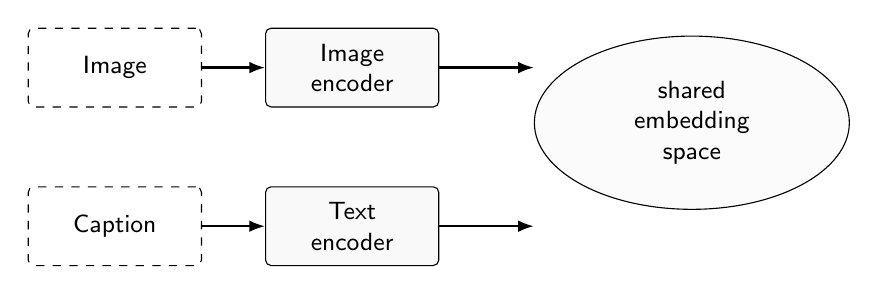
\begin{tikzpicture}[
    every node/.style={font=\small\sffamily},
    enc/.style={draw, rounded corners=2pt, minimum width=22mm, minimum height=10mm, align=center, fill=gray!5},
    inp/.style={draw, dashed, rounded corners=2pt, minimum width=22mm, minimum height=10mm, align=center},
    space/.style={draw, ellipse, minimum width=40mm, minimum height=22mm, align=center, fill=gray!3},
    arr/.style={-{Latex[length=2mm]}, thick}
]
\node[inp] (img) at (0,0) {Image};
\node[inp, below=10mm of img] (txt) {Caption};
\node[enc, right=8mm of img] (imgEnc) {Image\\encoder};
\node[enc, right=8mm of txt] (txtEnc) {Text\\encoder};
\node[space, right=12mm of imgEnc, yshift=-7mm] (sp) {shared\\embedding\\space};

\draw[arr] (img) -- (imgEnc);
\draw[arr] (txt) -- (txtEnc);
\draw[arr] (imgEnc) -- (sp.west |- imgEnc.east);
\draw[arr] (txtEnc) -- (sp.west |- txtEnc.east);
\end{tikzpicture}
\caption{The dual-encoder architecture of CLIP. Image and text encoders are trained jointly so that the embeddings of matching (image, caption) pairs lie close together in a shared space, while non-matching pairs are pushed apart.}
\label{fig:clip}
\end{figure}

Having established what CLIP produces, two practical questions remain: how the resulting vectors should be compared, and where they should be stored.

The image encoder used by the proposed application produces 512-dimensional embeddings. Whether such embeddings are compared by cosine similarity, Euclidean distance or inner product is in principle a free choice, but in practice these metrics are not all equivalent. Cosine similarity, defined as

\begin{equation}
\cos(u, v) = \frac{\langle u, v \rangle}{\|u\| \cdot \|v\|},
\label{eq:cosine}
\end{equation}

measures the angle between two vectors and ignores their magnitudes. When the embeddings are L2-normalised (i.e.~rescaled to unit norm), cosine similarity coincides exactly with their inner product, and Euclidean distance becomes a strictly monotonic function of cosine similarity:

\begin{equation}
\|u - v\|^2 = 2 \big(1 - \langle u, v \rangle\big) \quad \text{when } \|u\| = \|v\| = 1.
\label{eq:cos-l2-equiv}
\end{equation}

For this reason, the proposed application L2-normalises every embedding before storing it, which makes cosine, inner-product and (rank-equivalent) Euclidean retrieval interchangeable. Cosine is preferred because it is invariant to embedding magnitude, a property that matters whenever the encoder's output norm depends on the input in ways that should not influence retrieval. Table~\ref{tab:metrics} summarises the relationship between the three metrics.

\begin{table}[ht]
\centering
\caption{Distance and similarity metrics on embeddings.}
\label{tab:metrics}
\small
\renewcommand{\arraystretch}{1.3}
\begin{tabular}{@{}>{\raggedright\arraybackslash}p{3.0cm}
                  >{\raggedright\arraybackslash}p{4.2cm}
                  >{\raggedright\arraybackslash}p{2.8cm}
                  >{\raggedright\arraybackslash}p{3.0cm}@{}}
\toprule
\textbf{Metric} & \textbf{Formula} & \textbf{Magnitude-aware?} & \textbf{After L2 normalisation} \\
\midrule
Cosine similarity & \(\langle u, v \rangle / (\|u\| \cdot \|v\|)\) & no & equals inner product \\
\addlinespace[4pt]
Inner product     & \(\langle u, v \rangle\)                       & yes & equals cosine similarity \\
\addlinespace[4pt]
Euclidean distance & \(\|u - v\|\)                                 & yes & monotonic in cosine \\
\bottomrule
\end{tabular}
\end{table}

Once embeddings have been produced, they must be stored and queried. The proposed application uses the pgvector extension to PostgreSQL rather than a dedicated vector database such as Pinecone or Milvus; pgvector adds a \texttt{vector(n)} column type, distance operators for cosine, inner product and Euclidean metrics, and HNSW and IVFFlat indexes tied directly to the query planner. The choice is deliberate: small-retailer data volumes are modest (tens of thousands of items per active user, not the billions that justify a specialised store), and co-locating embeddings with the operational data lets a single transaction update a product, its embedding and its analytics, and lets retrieval combine with ordinary SQL filters (``similar products belonging to this user, not deleted, in stock'') in one query. Within this thesis, ``the vector index'' and ``the database'' therefore refer to the same PostgreSQL instance.

\section{Hybrid Generative--Deterministic Pipelines}
\label{sec:hybrid}

A generative model alone is insufficient whenever the output must remain truthful to a real, specific product: drift in colour, texture and silhouette is the rule rather than the exception. The way out, detailed in \textit{Chapter~\ref{chap:contributions}}, is to split the work between a generative phase that produces a background scene with explicit placeholder regions and a deterministic phase that pastes the actual product photographs into those regions and overlays the textual elements. The same split is exposed to the user as a toggle on product preservation: on, the generator designs only the background and the compositor places the products at pixel-level fidelity; off, the generator renders the products itself with more creative latitude, guided by but not bound to their original colour and shape.

For print export, the platform additionally upscales the finished asset with Real-ESRGAN \cite{wang2021realesrgan}; the full print pipeline is described in Section~\ref{sec:print-pipeline}.


\chapter{System Specification and Cloud Architecture}
\label{chap:architecture}

The platform's specification covers three layers: what it has to do, how its components fit together, and how it runs on Microsoft Azure as a production service. The recommendation engine and the hybrid generative pipeline appear here only as participants in the architecture; their internal workings are deferred to the contributions chapter that follows. Most of what the platform delivers happens around the AI calls rather than inside them, so the orchestration, the credit ledger, the tenant isolation and the admission boundary are the elements that determine what a retailer actually receives.

\section{Functional and Non-Functional Requirements}
\label{sec:requirements}

The objectives stated in Chapter~\ref{chap:introduction} establish what the platform exists to do. The present section translates those objectives into a set of requirements concrete enough to drive the architectural decisions that follow.

\subsection{Functional requirements}
\label{subsec:functional-requirements}

The functional requirements are organised by capability area. Each paragraph describes what the platform must let its users do, abstracted from how the capability is delivered.

\textbf{Identity and shop onboarding:} The platform must allow a retailer to create an account, authenticate, and complete a brief onboarding flow that captures the shop's identity. Onboarding is a three-stage process that captures, in turn, the shop's basic descriptors, its visual brand identity, and the contact details through which the shop reaches its customers. The parameters gathered here are not all mandatory at the point of generation: the retailer can decide, on a per-request basis, which of them to feed into the prompt and which to leave out, so that an asset can be made as specific or as generic as the situation calls for. Once onboarding is complete, the shop's currency and the language in which generated assets are to be produced are locked, and every subsequent generation request inherits both as default parameters.

\textbf{Product library:} Each retailer maintains a library of the products on offer. Each product carries a name, a category, a price and a representative photograph, and the retailer can create, edit and delete entries at will. The library is filterable by name, category and price range, and the lists it produces are consulted on every generation screen. Product photographs can also be cleaned up through a one-tap background-removal action, delegated to an external image-processing service, that replaces the original background with a transparent canvas suitable for compositing.

\textbf{Reference catalogue and search by photo:} Alongside the retailer's own library, the platform maintains a curated catalogue of professional product imagery covering the kinds of goods that small shops typically sell, such as snacks, drinks or household items, organised by a hierarchical category tree. When adding a product, the retailer takes a photograph of the real item with their phone and then chooses whether to keep that photograph as the product image or replace it with the closest match from the curated catalogue. The match is found by an internal AI model that compares the uploaded photograph against the catalogue's images, so a phone shot of, say, a coffee mug yields a small ranked list of catalogue mugs that look like it, without the retailer having to type a description. If a catalogue image is selected, it enters the retailer's library with the clean studio appearance that subsequent generation steps expect.

\textbf{Asset generation:}\label{par:asset-generation} The platform must produce three families of marketing imagery from the inputs gathered during onboarding and from the retailer's library. Announcements are single-product or single-event promotional posts, used to advertise a discount, a new arrival, a job opening or an upcoming store event. Catalogues are multi-product editorial layouts that gather a curated selection of the shop's offer into a single image, useful for seasonal campaigns or weekly highlights. Wallpapers are clean branded backdrops intended for in-store screens or social-media headers, where the shop's identity rather than any specific product is the focus.

Each family is parameterised by the brand context recorded at onboarding and by the locked language, so that the supported language variants can be produced on demand. The generation contract itself is model-agnostic: several multimodal providers sit behind a single abstraction, and the retailer picks one at the moment of each request. Each model carries a credit cost that reflects its computational class and per-call price, so the cost-versus-quality trade-off is visible to the retailer rather than hidden inside the orchestrator. The catalogue family in particular is produced by three generator flavours, summarised in Table~\ref{tab:catalogue-flavours}.

\begin{table}[ht]
\centering
\caption{Catalogue generator flavours.}
\label{tab:catalogue-flavours}
\small
\renewcommand{\arraystretch}{1.3}
\begin{tabularx}{\textwidth}{|>{\raggedright\arraybackslash}p{3.8cm}|Y|}
\hline
\textbf{Flavour} & \textbf{Description} \\
\hline
Fully generative & The multimodal model designs and renders the whole scene, products included. \\
\hline
Hybrid (preserve products) & The model renders the scene with reserved placeholder regions, and the platform's compositor pastes the retailer's actual product photographs into them so that product fidelity is preserved pixel for pixel. \\
\hline
In-house composite & No model is invoked at generation time, and the platform's deterministic compositor lays out the products, prices and brand identity directly onto a chosen background image. \\
\hline
\end{tabularx}
\end{table}

The announcement family is in turn sub-typed by post intent, with each sub-type carrying its own prompt template and required fields (Table~\ref{tab:announcement-subtypes}).

\begin{table}[ht]
\centering
\caption{Announcement sub-types.}
\label{tab:announcement-subtypes}
\small
\renewcommand{\arraystretch}{1.3}
\begin{tabularx}{\textwidth}{|>{\raggedright\arraybackslash}p{3.8cm}|Y|}
\hline
\textbf{Sub-type} & \textbf{Description} \\
\hline
Announcement & A general post for store news such as new arrivals, in-store events or schedule changes. \\
\hline
Job post & A hiring notice covering the open role, its responsibilities and the channel for applications. \\
\hline
Promotion & A discount-driven post advertising a price cut, coupon code or time-limited offer on selected products. \\
\hline
\end{tabularx}
\end{table}

The internal mechanics of the hybrid catalogue mode are deferred to the contributions chapter that follows.

\textbf{Daily marketing recommendations:} Once a day, the platform must produce a small ranked set of fresh marketing themes adapted to the retailer's shop and to the day's external context (weather, local events, holidays). Each theme is presented as a fully drafted promotional idea, in the locked language, and the retailer may either dismiss it, react to it, or hand it directly to the asset-generation pipeline as a starting prompt. The recommendation engine that produces these themes is the first of the two main contributions of this thesis and is described in detail in Chapter 4.

\textbf{Asset library and print export:} Every generated asset, regardless of family and mode, is persisted to the retailer's gallery, where it can be browsed and filtered by asset type, by date and by name. The gallery is the canonical record of everything the platform has produced for the shop. Any gallery item may be exported as a print-ready document, in paper sizes A6 to A3, at $300\,$dpi; if the source asset is below the target resolution, the platform's premium print pipeline upscales it through a learned super-resolution model before laying out the page.

\textbf{Billing and credit accounting:} Every generation that consumes a paid AI provider must be debited against a per-tenant credit balance. The ledger is consistency-critical: a debit is recorded only when the AI call succeeds, a refund is issued only when it fails, and no retailer can be charged for a call that produced no asset. Each billable call is therefore wrapped in an atomic debit-and-record block, and any provider failure triggers an automatic refund. A small administrative interface lets operators grant credits to tenants and inspect the ledger, which is currently the only way a retailer's balance can grow.

\textbf{Administration:} A small set of capabilities is reserved to operators with the administrative flag set on their account, giving them broad oversight of the platform's data and tenants when intervention is required. The administrative surface is deliberately spartan and lives inside the same client application as the retailer surface, with the privileged screens hidden from non-administrative accounts.

\begin{table}[ht]
\centering
\caption{Summary of functional requirements by capability area.}
\label{tab:functional-requirements}
\small
\renewcommand{\arraystretch}{1.3}
\begin{tabularx}{\textwidth}{|>{\raggedright\arraybackslash}p{3.6cm}|Y|}
\hline
\textbf{Capability area} & \textbf{Brief description} \\
\hline
Identity and onboarding & Account creation and a three-stage shop profile, with currency and language locked at the end. \\
\hline
Product library         & Create, edit and delete products with photographs, filters by name, category and price, and one-tap background removal. \\
\hline
Reference search        & Browse the curated catalogue, or match a phone photograph against it through an internal AI model. \\
\hline
Asset generation        & Announcements, catalogues and wallpapers, generated with a user-selected provider in fully generative or hybrid mode. \\
\hline
Daily recommendations   & Daily themed promotional ideas grounded in the shop profile and external context. \\
\hline
Library and print       & Persistent gallery with print-ready export from A6 to A3, upscaled by super-resolution when needed. \\
\hline
Billing                 & Transactional credit ledger with an atomic debit-and-record around every AI call. \\
\hline
Administration          & Broad operator oversight over platform data and tenants. \\
\hline
\end{tabularx}
\end{table}

\subsection{Non-functional requirements}
\label{subsec:nonfunctional-requirements}

\textbf{Performance:} Routine read and write operations must feel instantaneous, completing within a couple of hundred milliseconds from the client's perspective. Operations that depend on AI calls are inherently slower, taking seconds to tens of seconds, and cannot be served within a synchronous request. They are therefore modelled as asynchronous jobs, with the client showing a loading state while the work runs and notifying the user once the result is ready.

\textbf{Cost-awareness:} Every paid AI call has a non-trivial unit cost, so the platform must keep aggregate spend under control without surprising its retailers. The credit-and-coin model provides per-call backpressure and makes the cost-versus-quality trade-off explicit through credits weighted by the chosen model. A second layer of defence sits at the gateway, where rate-limit policies are configured per tenant and per endpoint class.

\textbf{Availability and graceful degradation:} The platform integrates several third-party services (multimodal image providers, a background-removal service, geocoding), each of which can fail or rate-limit independently of the others. When one of them is unavailable the platform must still complete useful work: a recommendation run must not be aborted if a single context-signal provider fails, an asset generation must produce an actionable error and refund the credit if the chosen image provider is down, and a geocoding failure must not block onboarding. The design therefore commits to per-integration isolation, retries with exponential backoff and circuit-breaker policies on every external HTTP call.

\textbf{Security:} The retailer-facing surface of the platform is open, in the sense that any retailer can sign up and use it; what is closed off is the operational side, where the development environment, the cloud-side secrets and the underlying Azure resources are reachable only through identities on an allow-list maintained inside Microsoft Entra ID. Retailer authentication and authorisation are a separate concern, handled inside the application once a request has reached the public surface. Once a request has been admitted, the platform must also guarantee that no retailer can read, modify or otherwise observe another retailer's data. Tenant identity is carried explicitly on every database query, on every blob-storage signed URL and on every cache key, and cross-tenant queries are not part of the normal API surface. The administrative endpoints constitute the only deliberate exception and are reachable only by accounts whose administrative flag is set.

\textbf{Localisation:} The platform supports two interface and generation languages, English and Romanian, with the chosen language locked at onboarding and carried as a flag on the user record, on the shop record and on every generated asset. Generated artefacts are stored alongside their translations rather than regenerated on language switch, so that toggling the interface language has no monetary cost. The choice between different currencies follows the same locking pattern.

\textbf{Auditability and maintainability:} Every request produces a structured log line carrying a tenant identifier and a request correlation identifier, and every external HTTP call propagates that correlation identifier downstream. Distributed traces are emitted for the multi-stage pipelines such as image generation and daily recommendations, so the latency of each stage can be examined in isolation. On the maintainability side, the source code is organised by feature folder, so a change to a single capability such as the wallet touches one area of the codebase and the dependency graph between feature areas is kept shallow.

\begin{table}[ht]
\centering
\caption{Non-functional requirements and the architectural mechanisms that satisfy them.}
\label{tab:nonfunctional-requirements}
\small
\renewcommand{\arraystretch}{1.3}
\begin{tabularx}{\textwidth}{|>{\raggedright\arraybackslash}p{4.0cm}|Y|}
\hline
\textbf{Requirement} & \textbf{Architectural mechanism} \\
\hline
Interactive read/write latency & On-device caching of the product list and gallery, plus a stateless API for horizontal scale-out. \\
\hline
Long-running AI work & Asynchronous job model with client-polled status. \\
\hline
Cost backpressure & Per-call credit debit and gateway rate limits per tenant. \\
\hline
Graceful degradation & Retry with backoff, circuit breakers and per-integration isolation. \\
\hline
Closed admission & Entra ID allow-list at the gateway. \\
\hline
Tenant isolation & Tenant-scoped queries, signed URLs and cache keys. \\
\hline
Localisation & Language flag carried end-to-end with pre-translated assets. \\
\hline
Auditability & Correlation IDs in logs and per-stage distributed traces. \\
\hline
\end{tabularx}
\end{table}

\section{High-Level Architecture}
\label{sec:high-level-architecture}

The platform is organised in three tiers. A \emph{client}, shipped to the retailer as a web, iOS and Android application from a single codebase, talks to a \emph{stateless application server} that mediates between the user-facing surface and the platform's external dependencies. The application server sits behind an \emph{API gateway} that handles admission, transport security and rate limiting. From there, the server orchestrates calls to a handful of third-party services (the chosen multimodal image provider, the background-removal service and the geocoding service) and persists state in a \emph{data plane} made of a relational database with a vector extension and a separate object store for binary assets. Figure~\ref{fig:three-tier} sketches the arrangement.

\begin{figure}[ht]
\centering
% --- self-contained palette (muted, print-friendly) ---
\definecolor{cInk}{HTML}{2E3440}    % text + arrows
\definecolor{cIndigo}{HTML}{3F4D8C} % clients / gateway
\definecolor{cSlate}{HTML}{4A5568}  % application server
\definecolor{cTeal}{HTML}{2E5F8C}   % data plane
\definecolor{cAmber}{HTML}{B07A1F}  % on-device cache
\definecolor{cGray}{HTML}{7C8390}   % external services
\resizebox{\textwidth}{!}{%
\begin{tikzpicture}[
    font=\sffamily\scriptsize,
    card/.style={draw=#1, line width=0.9pt, rounded corners=3pt, inner sep=0pt,
                 drop shadow={shadow xshift=0.5mm, shadow yshift=-0.5mm,
                              fill=black, opacity=0.12}},
    tab/.style={fill=#1, rounded corners=2.5pt, inner xsep=6pt, inner ysep=0pt,
                minimum height=5.2mm, anchor=south west,
                font=\sffamily\scriptsize\bfseries, text=white},
    cli/.style={draw=cIndigo, line width=0.6pt, rounded corners=2.5pt, fill=white,
                minimum width=28mm, minimum height=7.5mm, align=center, text=cInk},
    chip/.style={draw=cSlate, line width=0.6pt, rounded corners=2.5pt, fill=white,
                 text width=21.5mm, minimum height=9.5mm, align=center,
                 inner xsep=3pt, text=cInk},
    store/.style={draw=cTeal, line width=0.6pt, cylinder, shape border rotate=90,
                  aspect=0.22, minimum width=26mm, minimum height=12mm, align=center,
                  cylinder uses custom fill, cylinder body fill=white,
                  cylinder end fill=cTeal!15, text=cInk},
    ext/.style={draw=cGray, line width=0.6pt, dash pattern=on 2.4pt off 1.7pt,
                rounded corners=2.5pt, fill=white, minimum width=28mm,
                minimum height=7.5mm, align=center, text=cInk},
    arr/.style={-{Latex[length=2mm,width=1.5mm]}, line width=0.7pt, draw=cInk!85}
]

% ============ tier cards (drawn first, content on top) ============
\node[card=cIndigo, fill=cIndigo!7, minimum width=110mm, minimum height=29.5mm]
      (clientsCard) at (9.8,10.925) {};
\node[card=cSlate, fill=cSlate!8, minimum width=110mm, minimum height=30.5mm]
      (serverCard) at (9.8,5.375) {};
\node[card=cTeal, fill=cTeal!8, minimum width=110mm, minimum height=20.5mm]
      (dataCard) at (9.8,1.575) {};
\node[draw=cGray, line width=0.9pt, dash pattern=on 2.4pt off 1.7pt,
      rounded corners=3pt, inner sep=0pt, fill=cGray!6,
      minimum width=36mm, minimum height=34.5mm]
      (extCard) at (1.8,5.375) {};

% ============ card header tabs ============
\node[tab=cIndigo] at ([xshift=4mm]clientsCard.north west) {Clients};
\node[tab=cSlate, minimum height=7.5mm, align=left]
      at ([xshift=4mm]serverCard.north west)
      {Application server\\(.NET, Semantic Kernel)};
\node[tab=cTeal] at ([xshift=4mm]dataCard.north west) {Data plane};
\node[tab=cGray] at ([xshift=4mm]extCard.north west) {External services};

% ============ clients tier ============
\node[draw=cAmber, line width=0.6pt, rounded corners=2.5pt, fill=cAmber!14,
      minimum width=102mm, minimum height=8.5mm, align=center, text=cInk]
      (cache) at (9.8,11.6)
      {On-device cache, one per device:\\product list and gallery (cleared on writes)};
\node[cli] (web)     at (6.1,10.2)  {Web client};
\node[cli] (ios)     at (9.8,10.2)  {iOS client};
\node[cli] (android) at (13.5,10.2) {Android client};

% ============ API gateway ============
\node[draw=cIndigo, line width=0.9pt, rounded corners=3pt, fill=cIndigo!14,
      minimum width=86mm, minimum height=8mm, align=center, text=cInk,
      drop shadow={shadow xshift=0.5mm, shadow yshift=-0.5mm,
                   fill=black, opacity=0.12}]
      (gw) at (9.8,8.45) {API gateway (TLS, CORS, rate limits)};

% ============ application server: feature services ============
\node[chip] (auth)    at (5.75,6.025)  {Auth};
\node[chip] (shop)    at (8.45,6.025)  {Shop profile};
\node[chip] (prod)    at (11.15,6.025) {Product library};
\node[chip] (gallery) at (13.85,6.025) {Gallery};
\node[chip] (refs)    at (5.75,4.725)  {Reference\\search};
\node[chip] (gen)     at (8.45,4.725)  {Image\\generation};
\node[chip] (reco)    at (11.15,4.725) {Recommendation\\engine};
\node[chip] (bill)    at (13.85,4.725) {Billing\\(credits)};

% ============ data plane ============
\node[store] (db)   at (8.1,1.575)  {PostgreSQL\\+ pgvector};
\node[store] (blob) at (11.5,1.575) {Blob storage};

% ============ external services ============
\node[ext] (ai)  at (1.8,6.425) {Multimodal AI\\providers};
\node[ext] (bg)  at (1.8,5.375) {Background\\removal};
\node[ext] (geo) at (1.8,4.325) {Geocoding};

% ============ arrows ============
% clients read from their on-device cache
\draw[arr] (cache.south -| web)     -- (web.north);
\draw[arr] (cache.south -| ios)     -- (ios.north);
\draw[arr] (cache.south -| android) -- (android.north);
% clients to gateway
\draw[arr] (web)     -- (web     |- gw.north);
\draw[arr] (ios)     -- (gw.north);
\draw[arr] (android) -- (android |- gw.north);
% gateway to application server
\draw[arr] (gw.south) -- (serverCard.north);
% server to data plane
\draw[arr] (serverCard.south -| db.north)   -- (db.north);
\draw[arr] (serverCard.south -| blob.north) -- (blob.north);
% external services to server
\draw[arr] (ai.east)  -- (serverCard.west |- ai);
\draw[arr] (bg.east)  -- (serverCard.west |- bg);
\draw[arr] (geo.east) -- (serverCard.west |- geo);

\end{tikzpicture}%
}
\caption{High-level architecture of the platform.}
\label{fig:three-tier}
\end{figure}

The application server is deliberately stateless. Every request carries the credentials by which the platform identifies the retailer, and the server keeps no in-memory session beyond the lifetime of the request itself. The arrangement lets the server scale horizontally without coordination, and it keeps every piece of surviving state in the data plane where transactional consistency is the database's job rather than the application's.

Two request shapes are supported. A \emph{synchronous} request is served end-to-end while the client waits and is used for routine reads and writes such as logging in or listing products. An \emph{asynchronous job} request is used for any operation whose work is dominated by long-running external calls. The server returns a job identifier as soon as the work is queued, and the client polls a status endpoint until the result is ready. Figure~\ref{fig:request-flows} contrasts the two flows.

\begin{figure}[ht]
\centering
% --- same palette as Figure \ref{fig:three-tier} ---
\definecolor{cInk}{HTML}{2E3440}    % text + arrows
\definecolor{cIndigo}{HTML}{3F4D8C} % client
\definecolor{cSlate}{HTML}{4A5568}  % server
\begin{minipage}[t]{0.46\textwidth}
\centering
\begin{tikzpicture}[
    baseline=(cl.north),
    font=\sffamily\scriptsize,
    actor/.style={draw=#1, line width=0.6pt, rounded corners=2.5pt, fill=white,
                  minimum width=17mm, minimum height=6.5mm, align=center, text=cInk},
    life/.style={draw=cInk!35, line width=0.6pt, dash pattern=on 2.4pt off 1.7pt},
    arr/.style={-{Latex[length=2mm,width=1.5mm]}, line width=0.7pt, draw=cInk!85},
    every node/.style={text=cInk}
]
\node[actor=cIndigo] (cl) at (0,0)   {Client};
\node[actor=cSlate]  (sv) at (3.4,0) {Server};
\draw[life] (cl.south) -- (0,-2.6);
\draw[life] (sv.south) -- (3.4,-2.6);
\draw[arr] (0,-1.0)   -- node[above]{request}  (3.4,-1.0);
\draw[arr] (3.4,-2.0) -- node[above]{response} (0,-2.0);
\node[align=center, text=cInk!75] at (1.7,-3.0) {\itshape synchronous};
\end{tikzpicture}
\end{minipage}\hfill
\begin{minipage}[t]{0.46\textwidth}
\centering
\begin{tikzpicture}[
    baseline=(cl.north),
    font=\sffamily\scriptsize,
    actor/.style={draw=#1, line width=0.6pt, rounded corners=2.5pt, fill=white,
                  minimum width=17mm, minimum height=6.5mm, align=center, text=cInk},
    life/.style={draw=cInk!35, line width=0.6pt, dash pattern=on 2.4pt off 1.7pt},
    arr/.style={-{Latex[length=2mm,width=1.5mm]}, line width=0.7pt, draw=cInk!85},
    every node/.style={text=cInk}
]
\node[actor=cIndigo] (cl) at (0,0)   {Client};
\node[actor=cSlate]  (sv) at (3.4,0) {Server};
\draw[life] (cl.south) -- (0,-4.45);
\draw[life] (sv.south) -- (3.4,-4.45);
\draw[arr] (0,-0.9)    -- node[above]{submit}  (3.4,-0.9);
\draw[arr] (3.4,-1.45) -- node[above]{job id}  (0,-1.45);
\draw[arr] (0,-2.25)   -- node[above]{poll}    (3.4,-2.25);
\draw[arr] (3.4,-2.8)  -- node[above]{pending} (0,-2.8);
\draw[arr] (0,-3.6)    -- node[above]{poll}    (3.4,-3.6);
\draw[arr] (3.4,-4.15) -- node[above]{result}  (0,-4.15);
\node[align=center, text=cInk!75] at (1.7,-4.85) {\itshape asynchronous job};
\end{tikzpicture}
\end{minipage}
\caption{The two request shapes supported by the platform. Synchronous requests are served while the client waits; asynchronous job requests return immediately with a job identifier, and the client polls a status endpoint until the result is available.}
\label{fig:request-flows}
\end{figure}

It is useful to record the implementation technologies once. The client is built with React Native \cite{reactnative} (Expo), which lets a single TypeScript codebase be exported as a static web build, an iOS application and an Android application. The server is an ASP.NET Core minimal-API service running on .NET 10. The data plane consists of PostgreSQL 18 with the pgvector extension and Microsoft Azure Blob Storage. React Native was chosen to keep a single codebase for the heterogeneous device population of the target audience, and ASP.NET Core was chosen because it has first-class support for the Semantic Kernel orchestration framework, which the platform's language-model reasoning relies on.

\section{Client Tier}
\label{sec:client-tier}

The client is the only tier the retailer ever sees directly, and it is the surface for all data entry, asset review and administrative operations.

Behind that surface the client is a thin shell over the remote API, with almost no domain logic of its own. Shared interface state lives in a small number of context providers (authentication, theme, shop profile, in-progress onboarding form) whose role is to hold values that several screens need to read in common. A single API client at the network boundary attaches the access token to every outgoing request, refreshes that token transparently when it expires, and translates server responses into the typed shapes that the rest of the codebase consumes.

Because almost every action costs real credits on the server side, the client takes a conservative line on optimistic UI: a write is reflected to the user only once it has been confirmed by the server.

The route tree mirrors the platform's user model. Unauthenticated routes serve registration and login. An onboarding group leads first-time accounts through the shop-profile setup and refuses to release them to the rest of the application until it is complete. The main set of tabs covers the home screen, the products library, the gallery, asset creation, the wallet and the profile. An administrative group hidden behind a flag exposes the operator capabilities.

\label{subsec:client-ui}
The retailer's first encounter with the platform is a sign-in screen with the option to register a new account. A first-time account is then led through the three-stage shop onboarding, and the rest of the application is unlocked only once the profile has been recorded.

\begin{figure}[!ht]
\centering
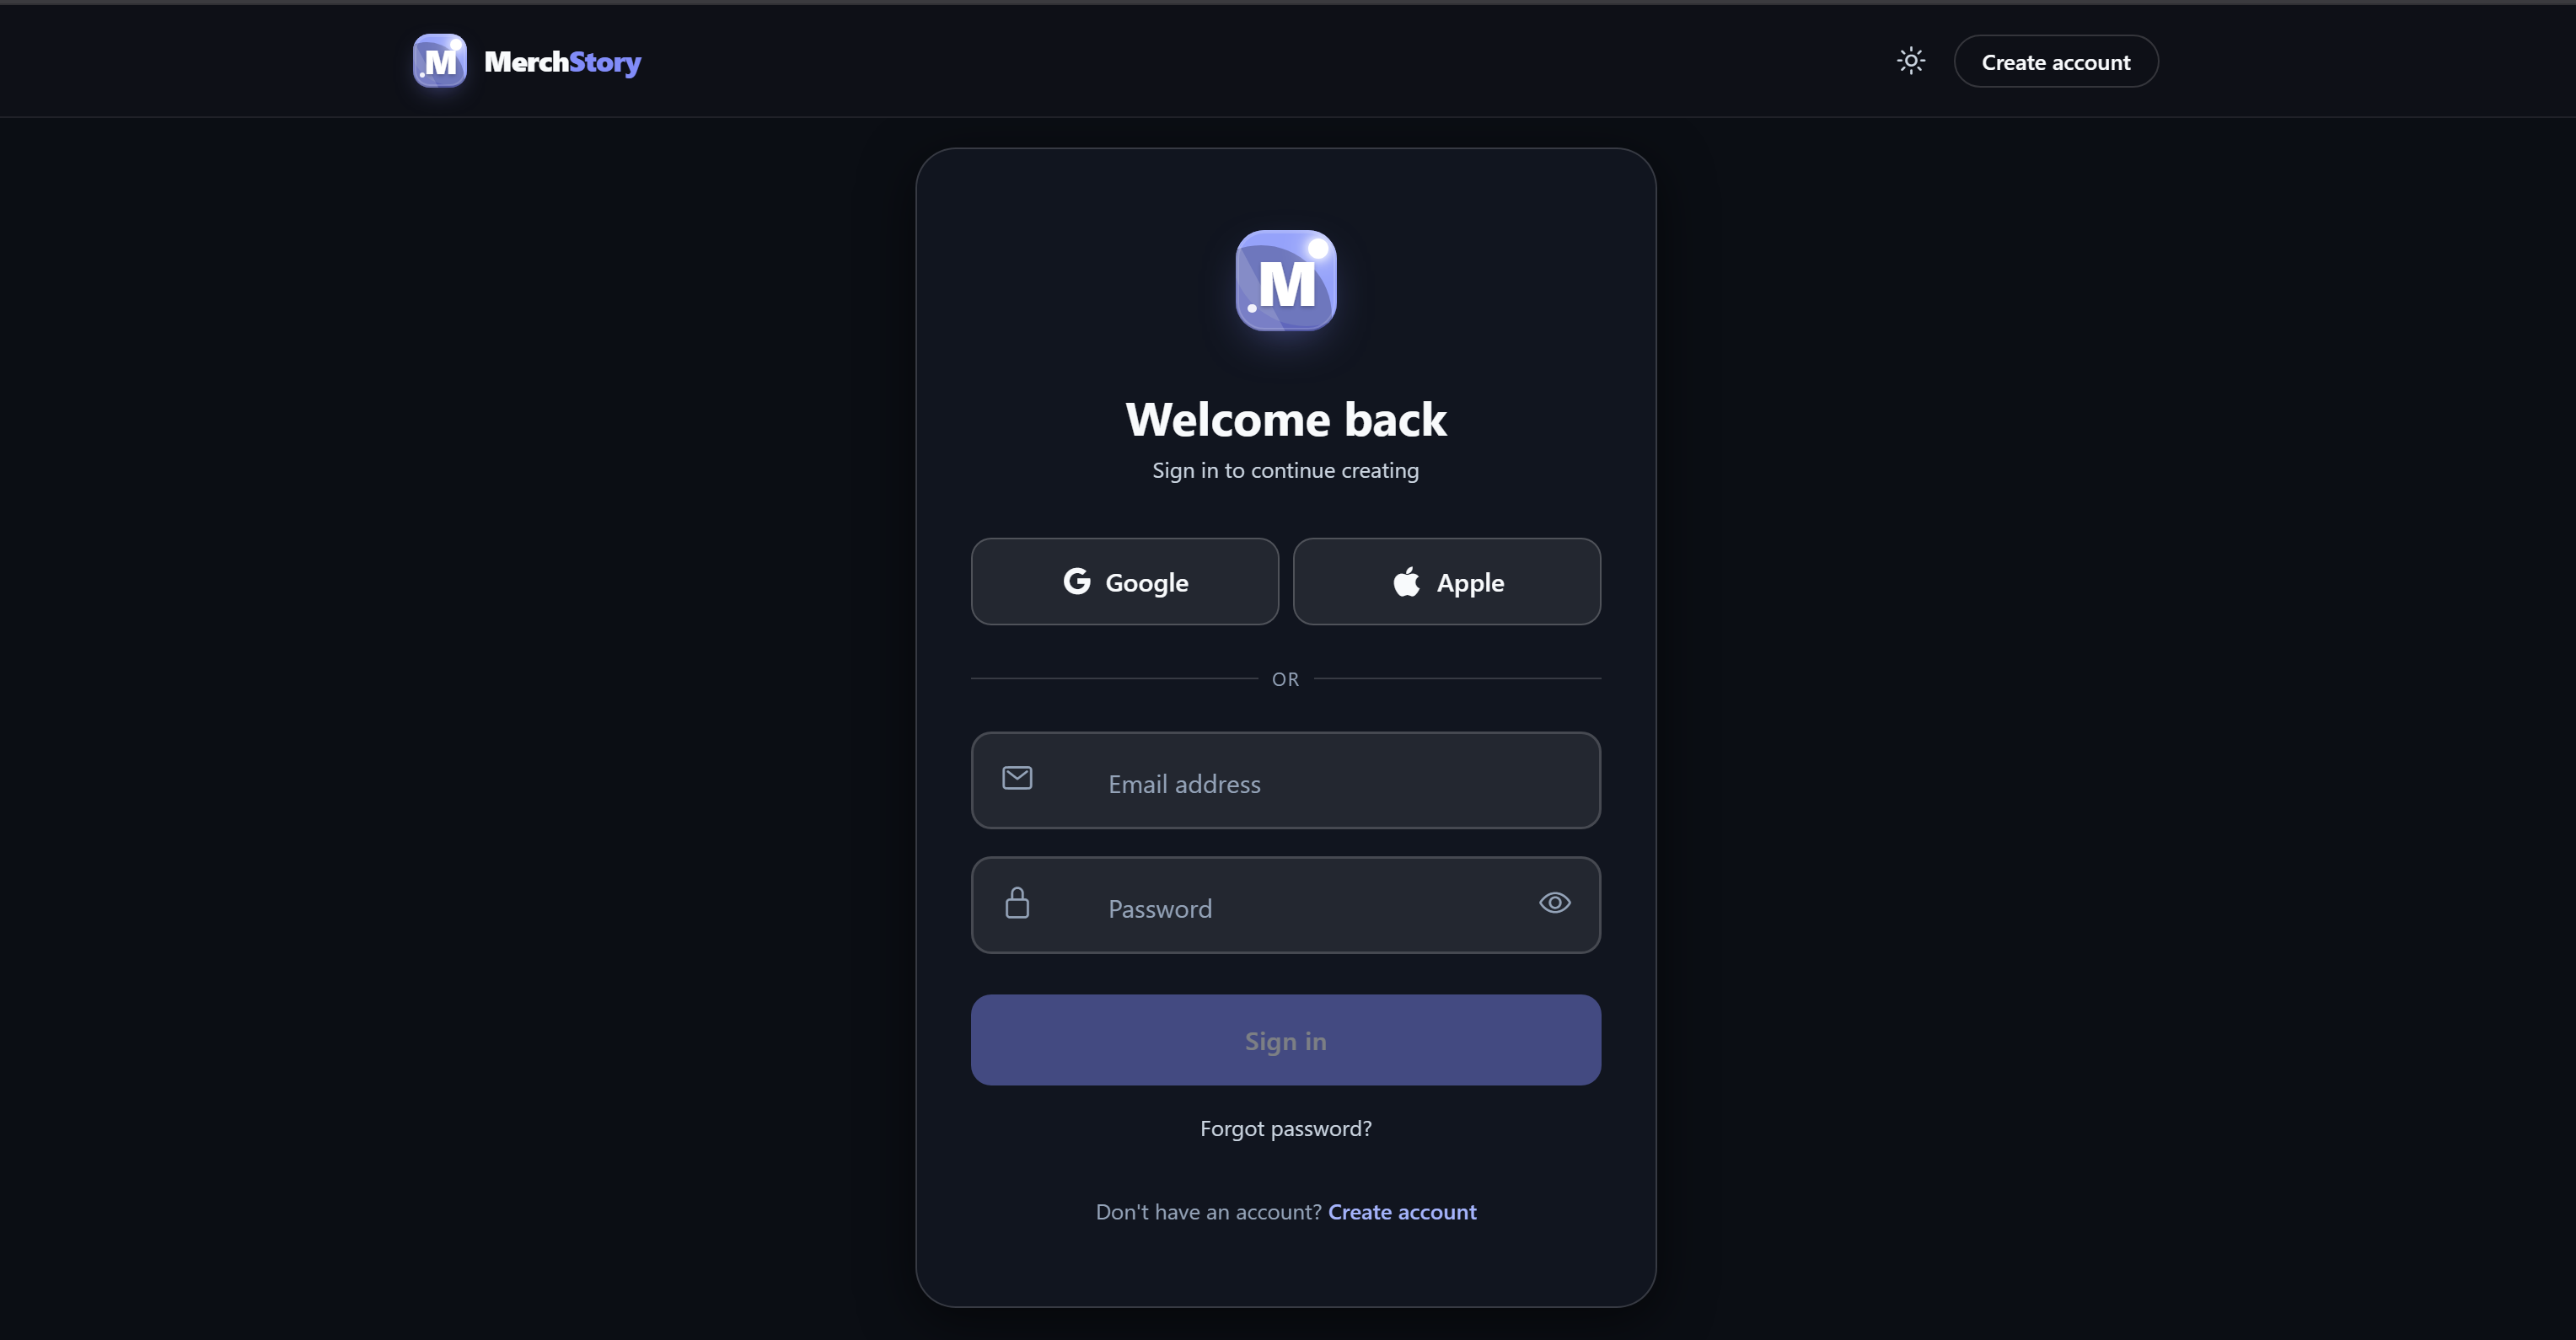
\includegraphics[height=0.28\textwidth]{figures/client/login.png}\hfill
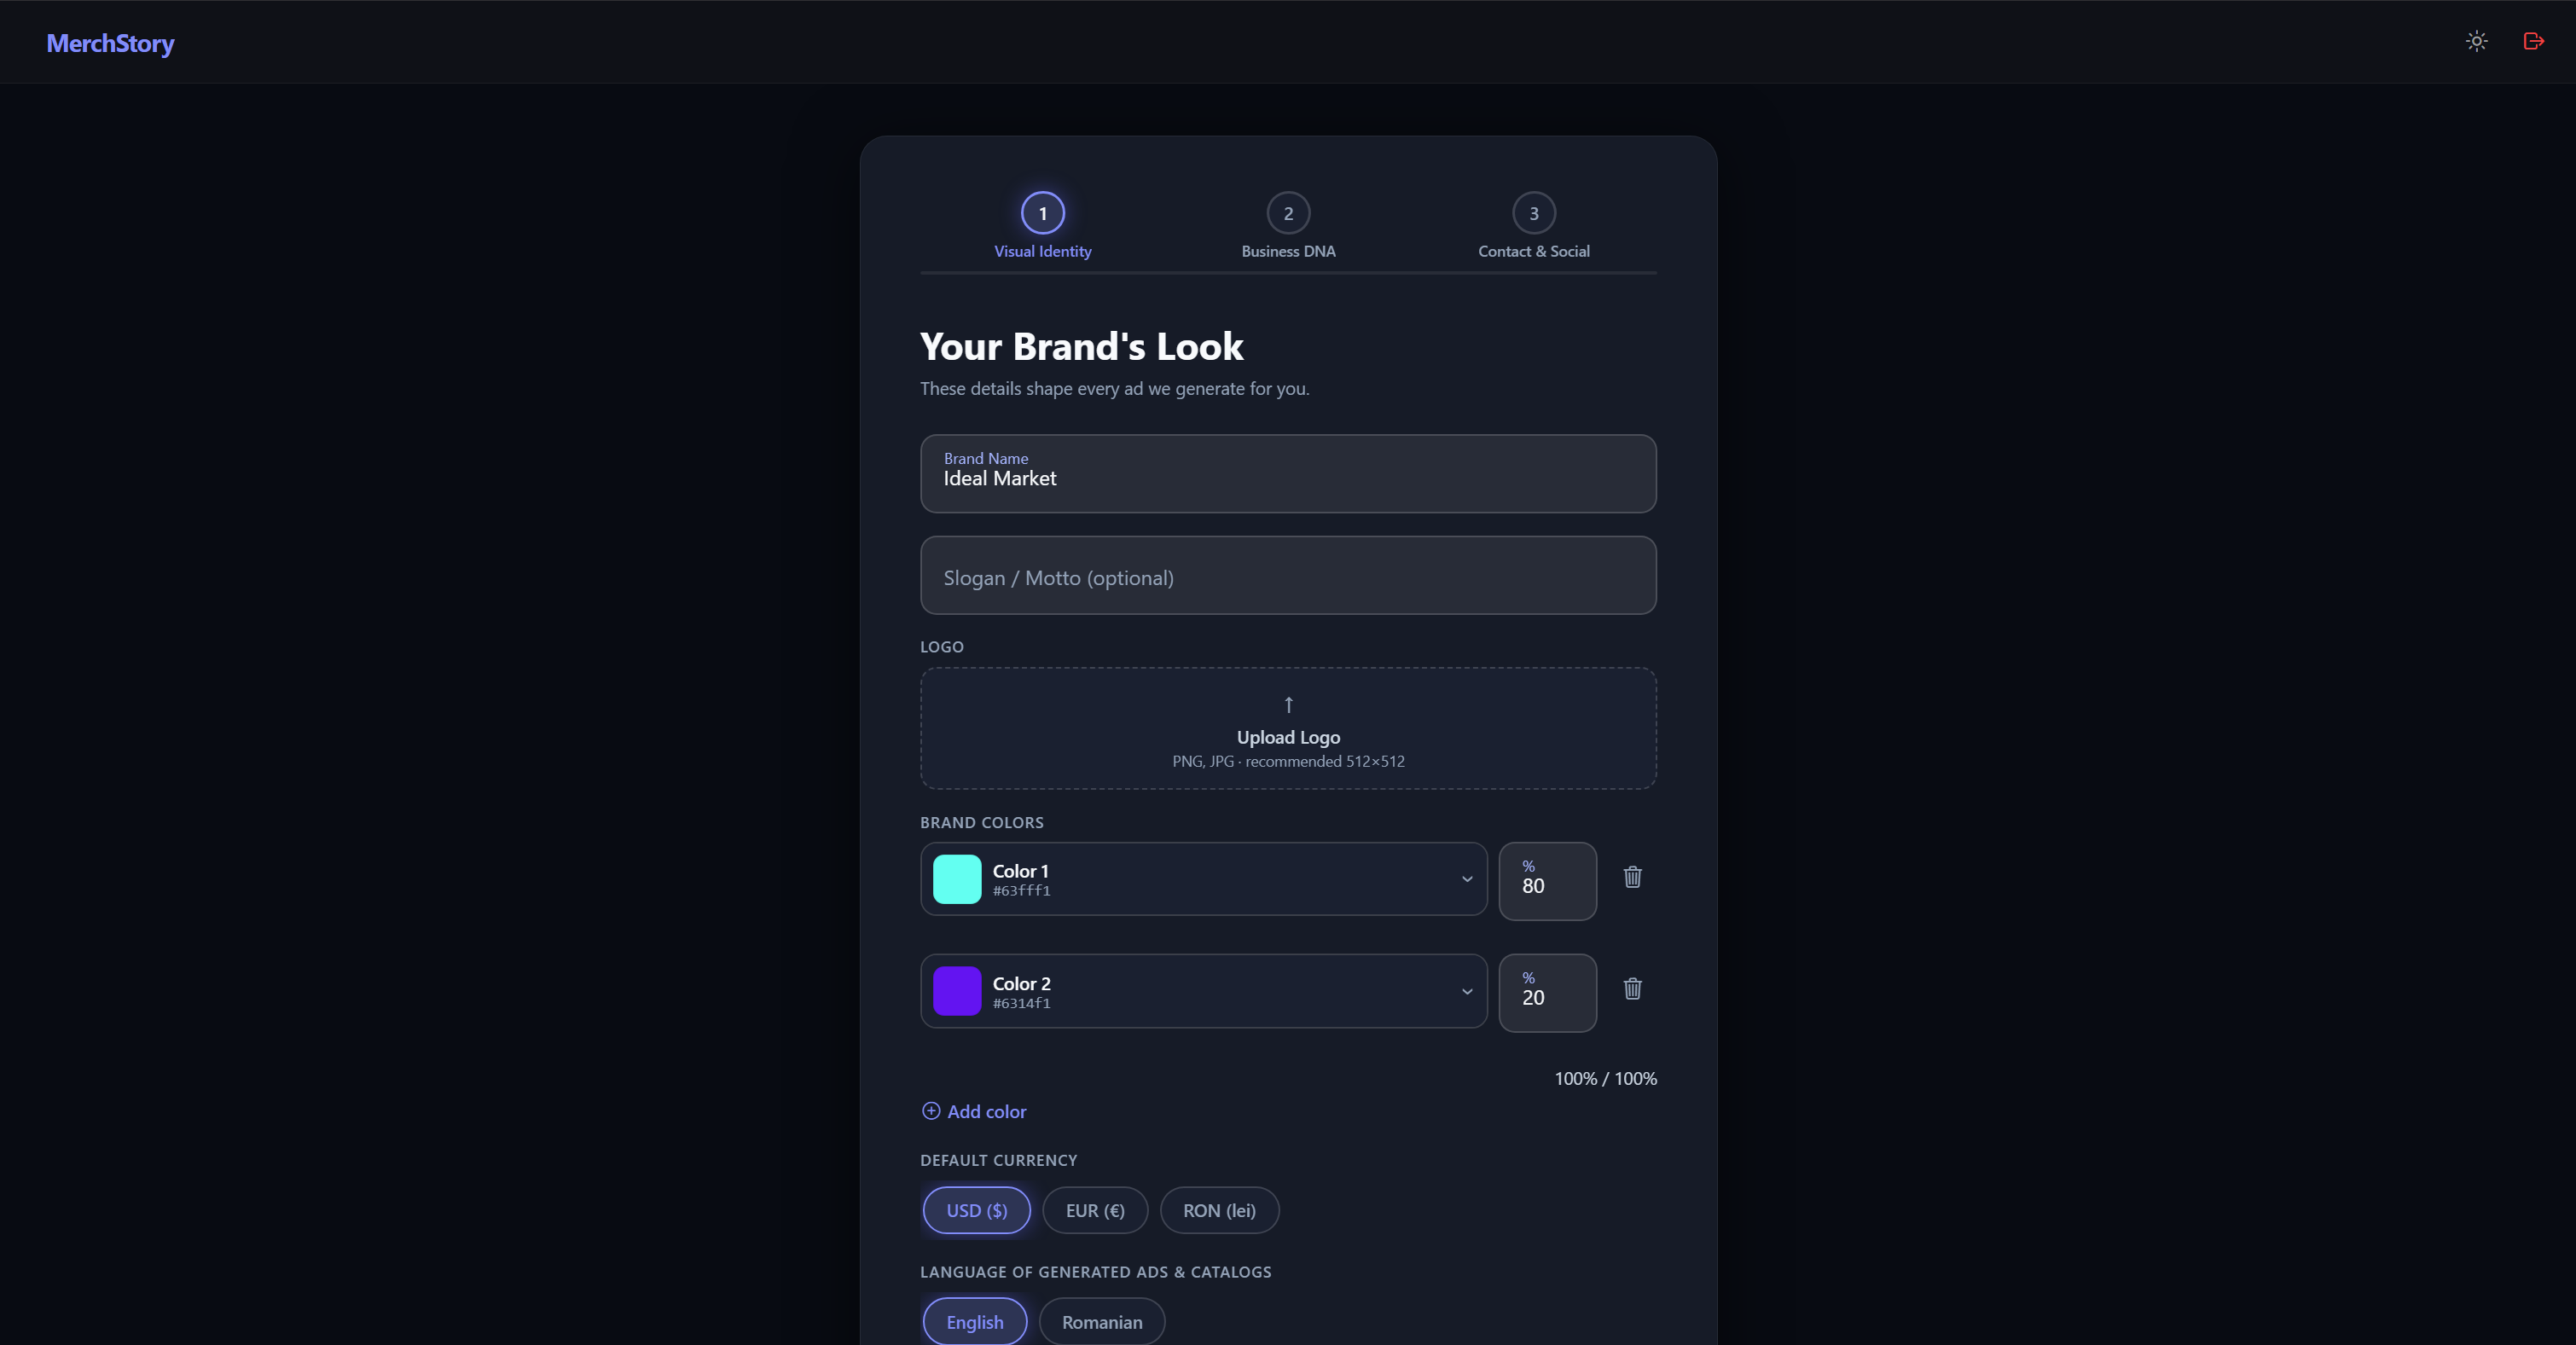
\includegraphics[height=0.28\textwidth]{figures/client/onboarding.png}
\caption{Login screen and shop onboarding step.}
\label{fig:client-auth}
\end{figure}

Once onboarding is complete, the retailer lands on the home surface, a tab bar that gives one-tap access to the main parts of the application. Asset creation is the heart of the daily workflow: the retailer chooses an asset family, picks the products to feature and the model to use, and is shown an explicit progress indicator while the generation runs in the background.

\begin{figure}[!ht]
\centering
\begin{minipage}[t]{0.48\textwidth}
\centering
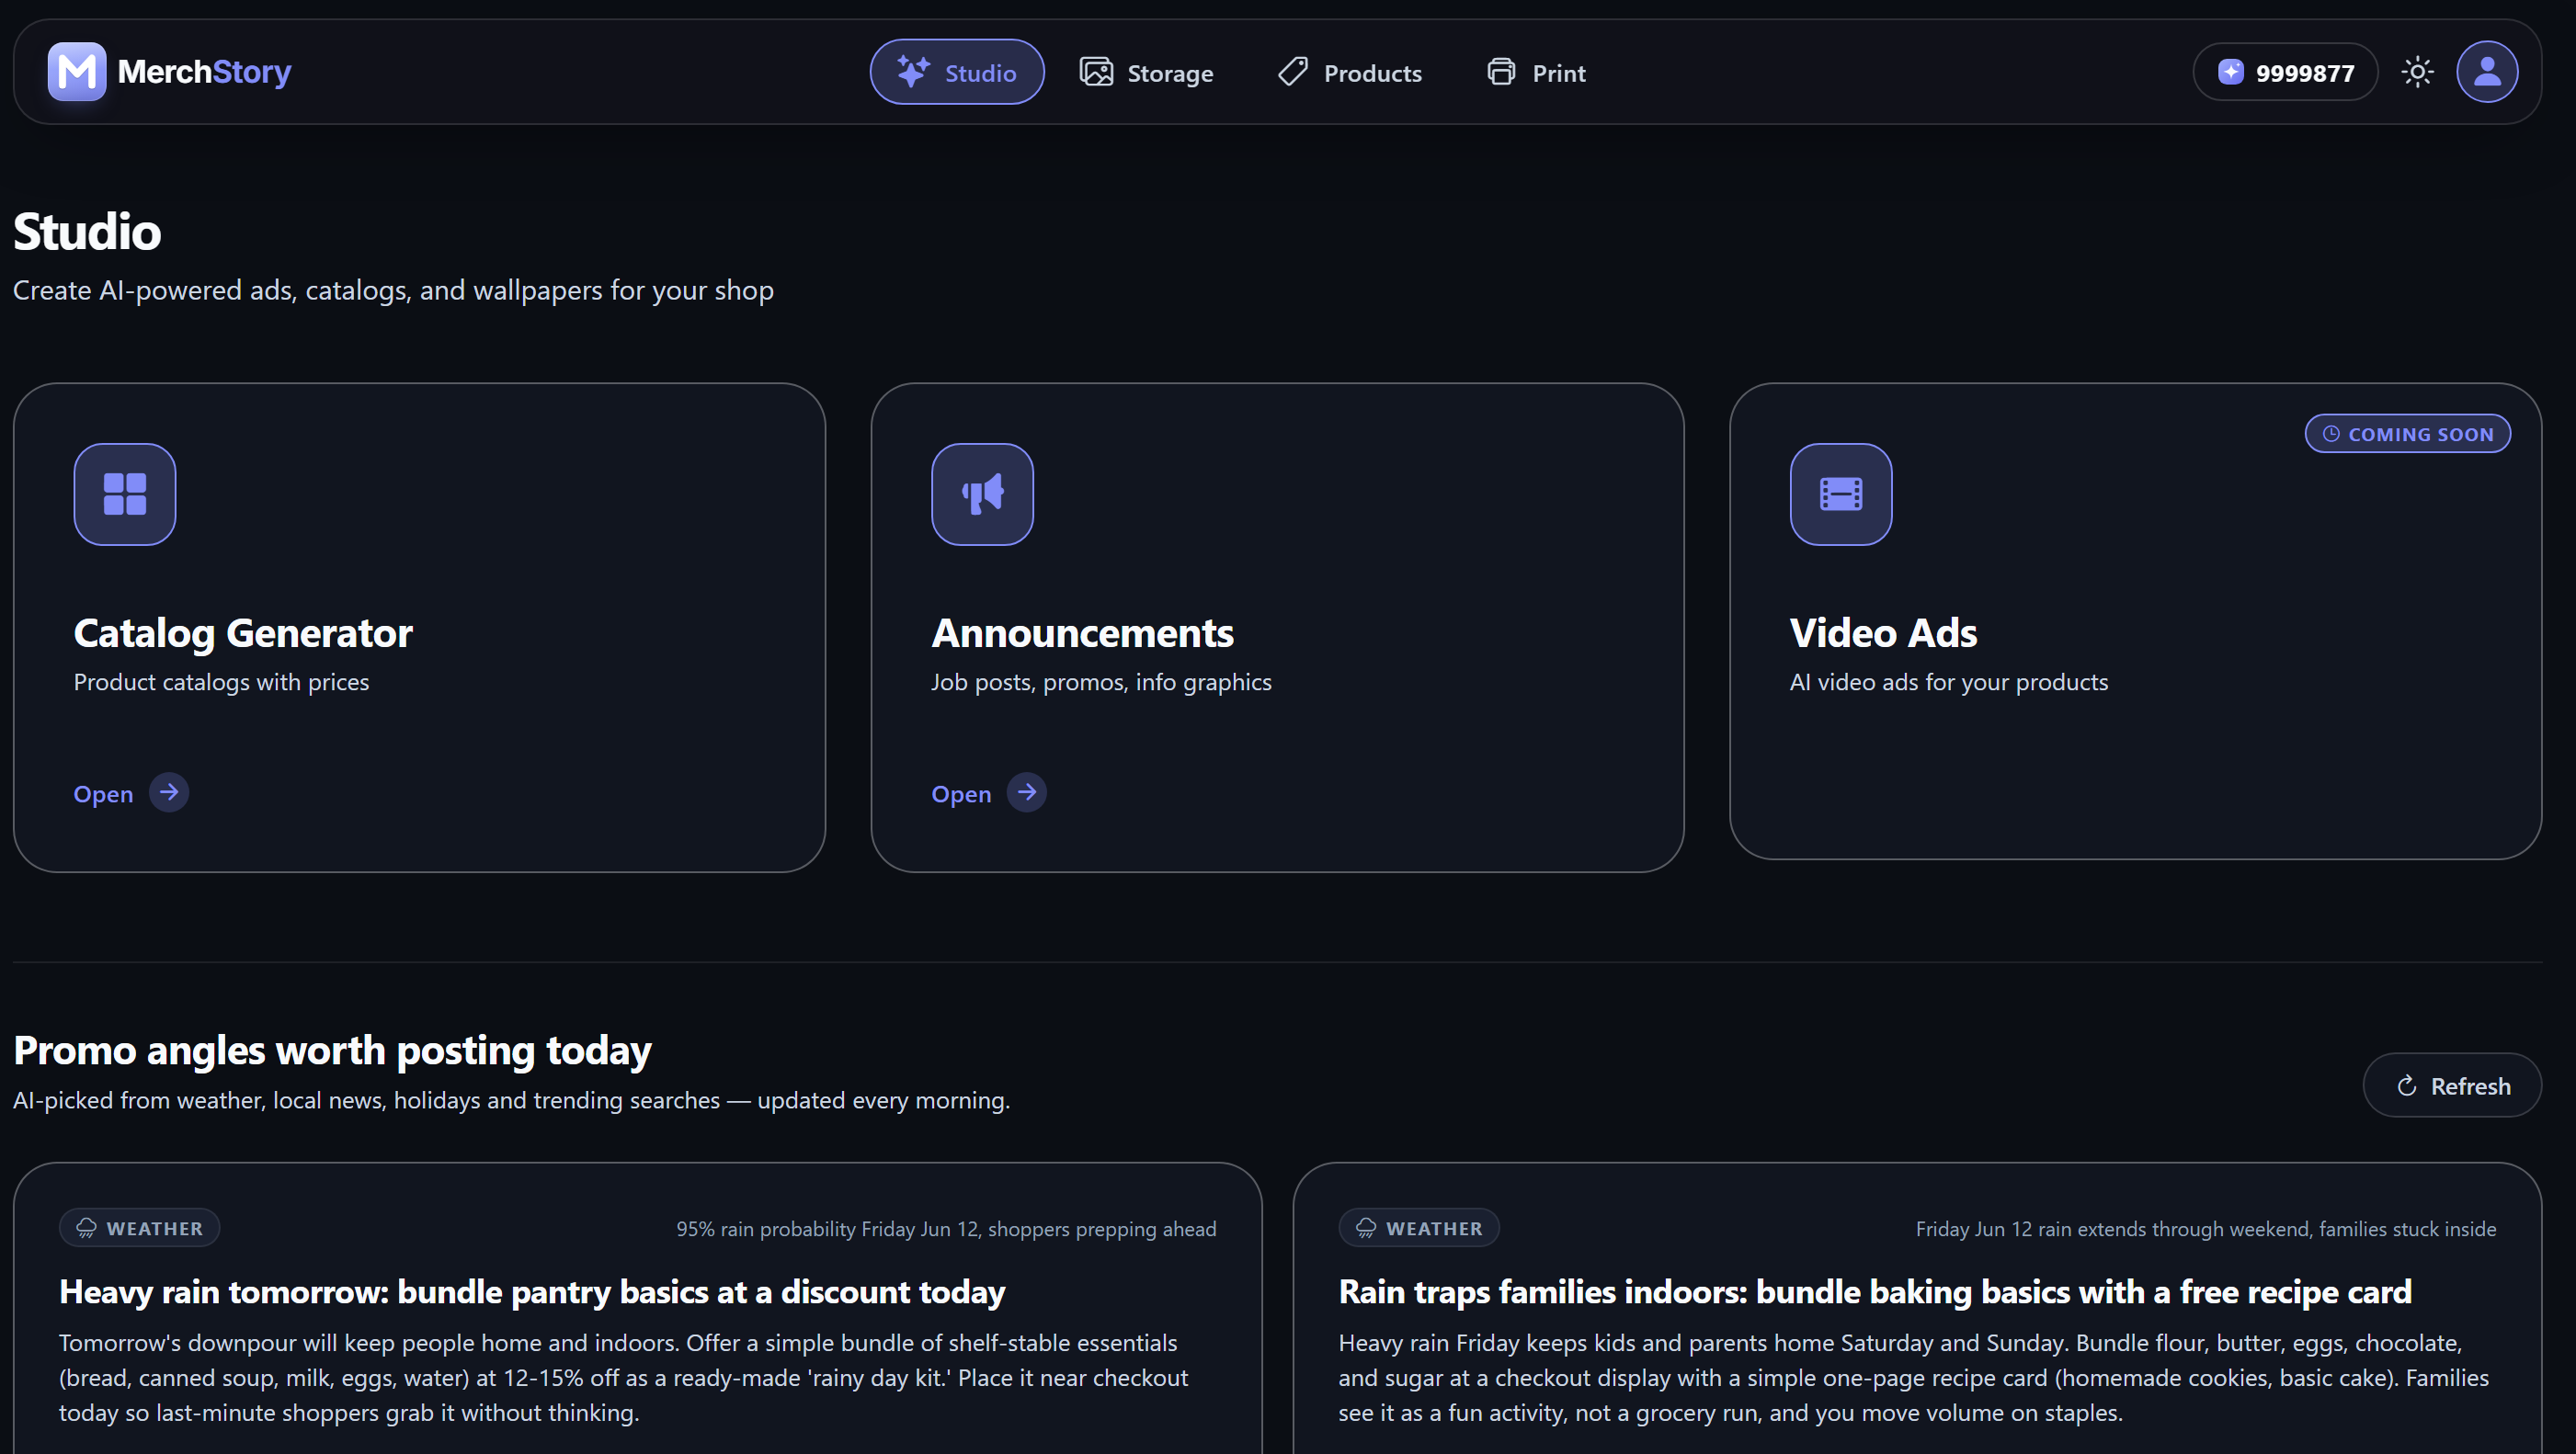
\includegraphics[width=\linewidth]{figures/client/home.png}
\end{minipage}\hfill
\begin{minipage}[t]{0.48\textwidth}
\centering
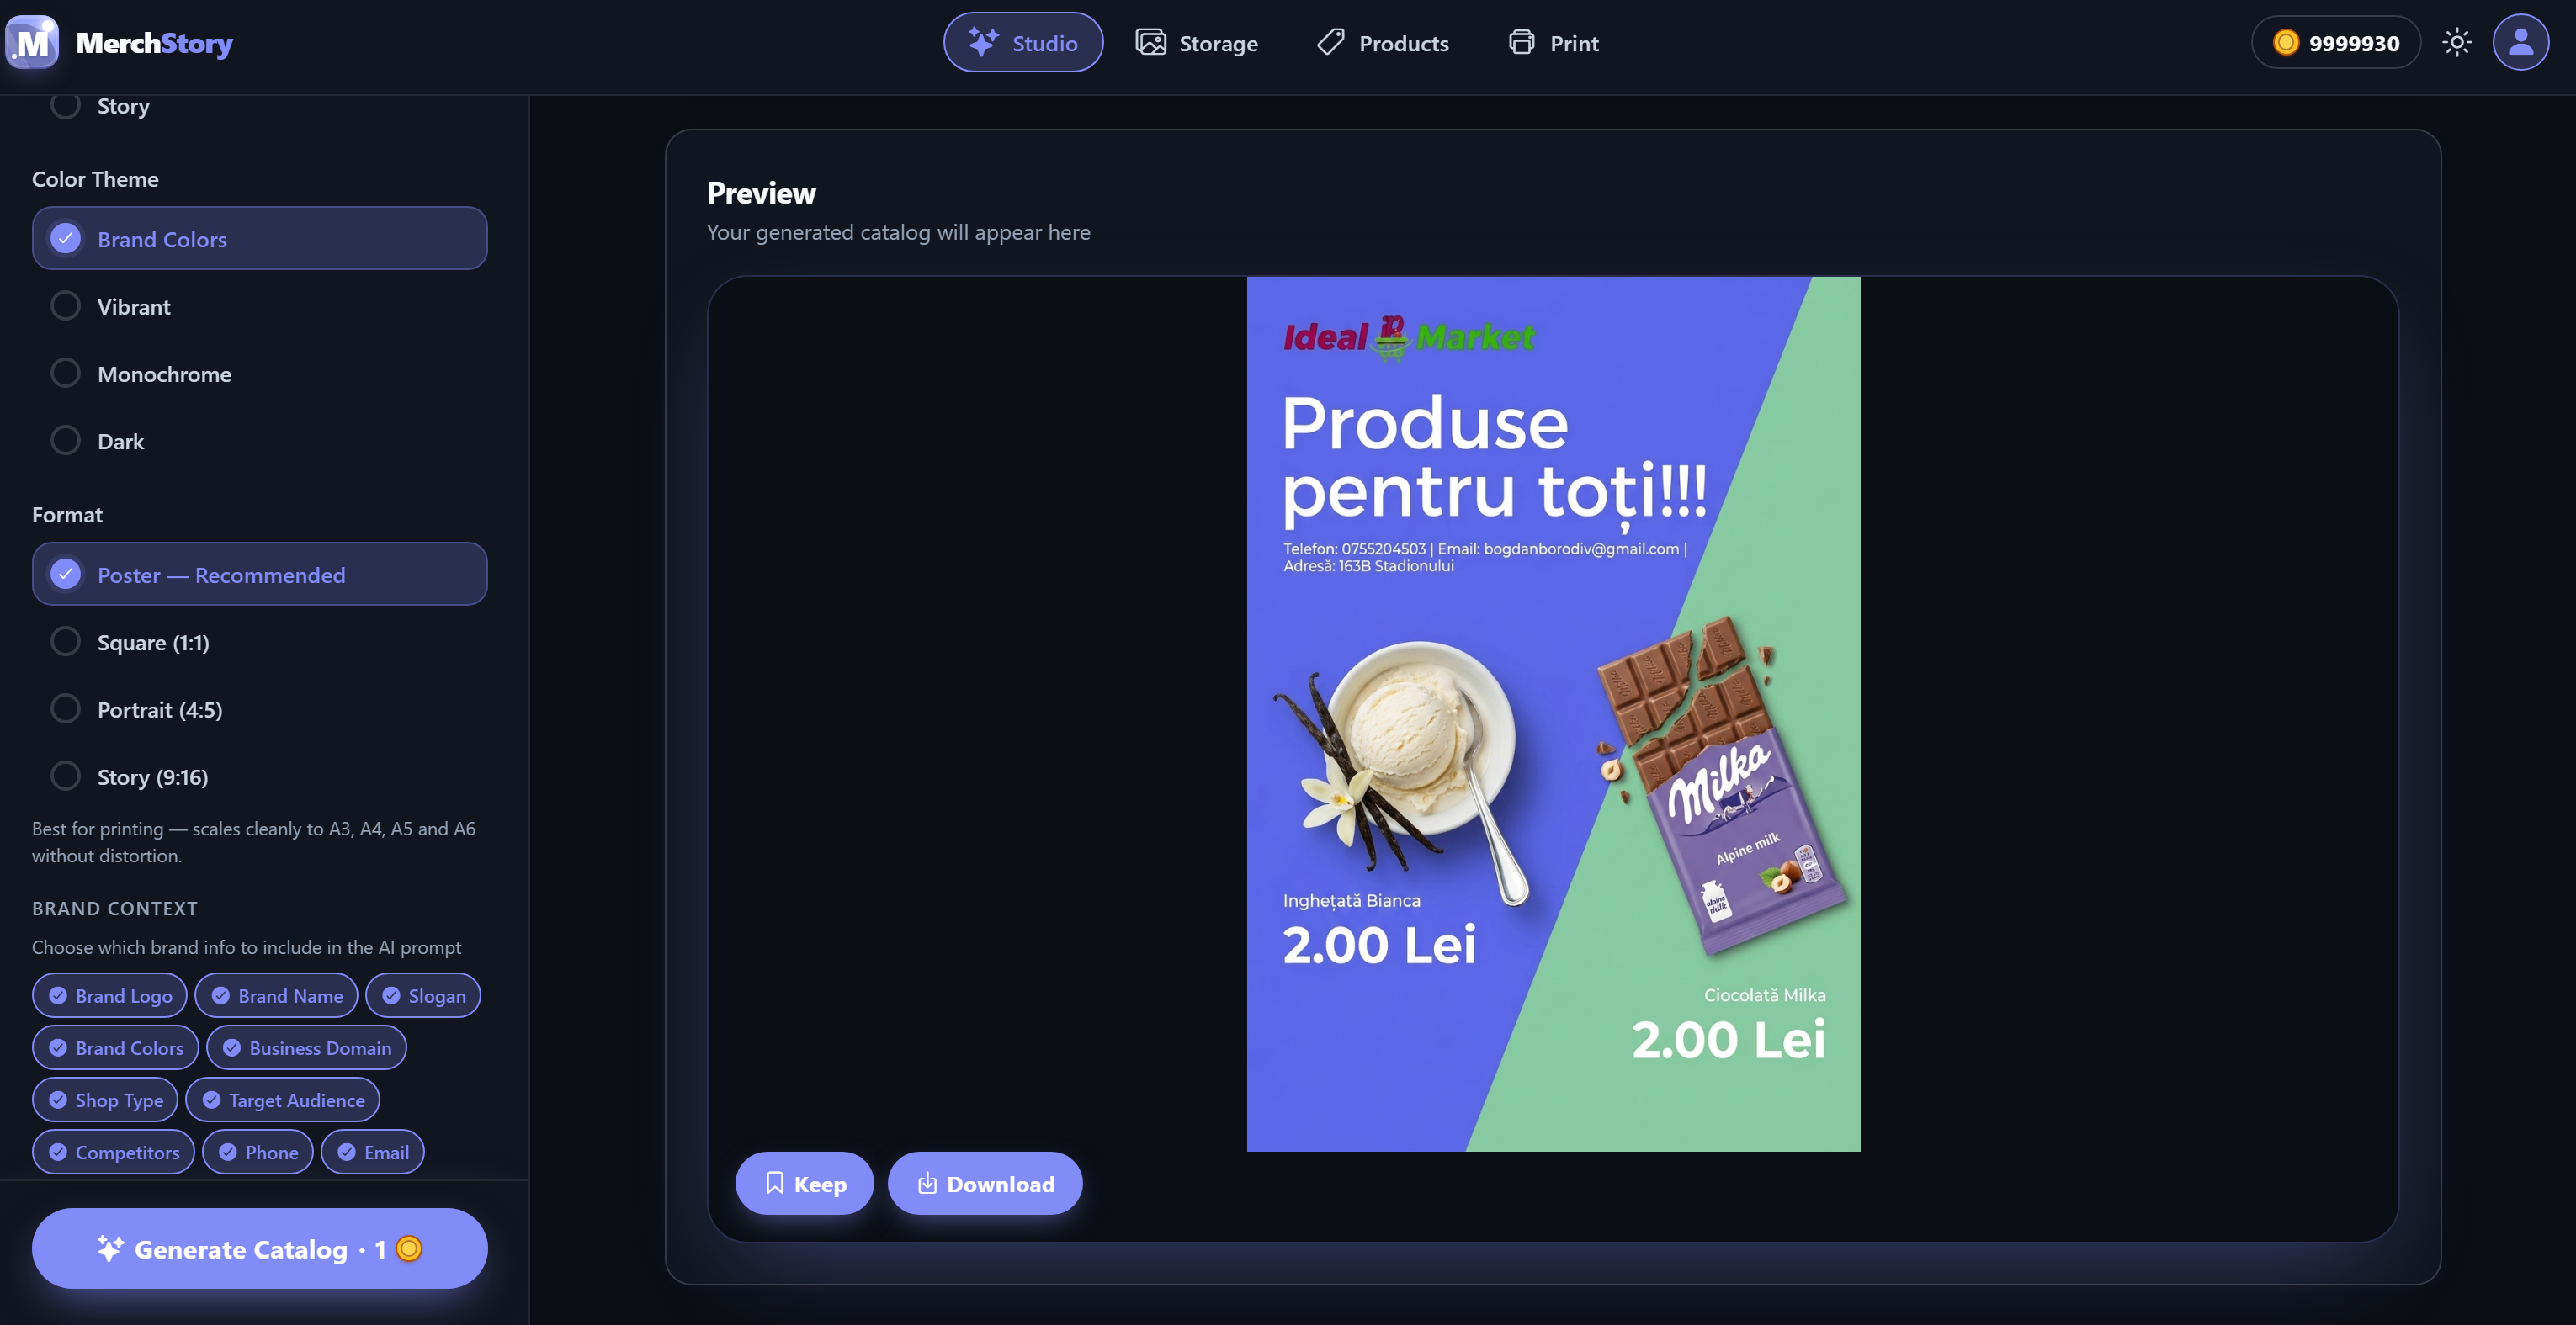
\includegraphics[width=\linewidth]{figures/client/asset-creation.png}
\end{minipage}
\caption{Home tabs and the asset-creation flow.}
\label{fig:client-main}
\end{figure}

Every generated asset is collected in the gallery, where the retailer can browse, filter and export past work. The wallet shows the credit balance and the history of debits and refunds, so the cost of each generation is visible and auditable from the same tab bar.

\begin{figure}[!ht]
\centering
\begin{minipage}[t]{0.48\textwidth}
\centering
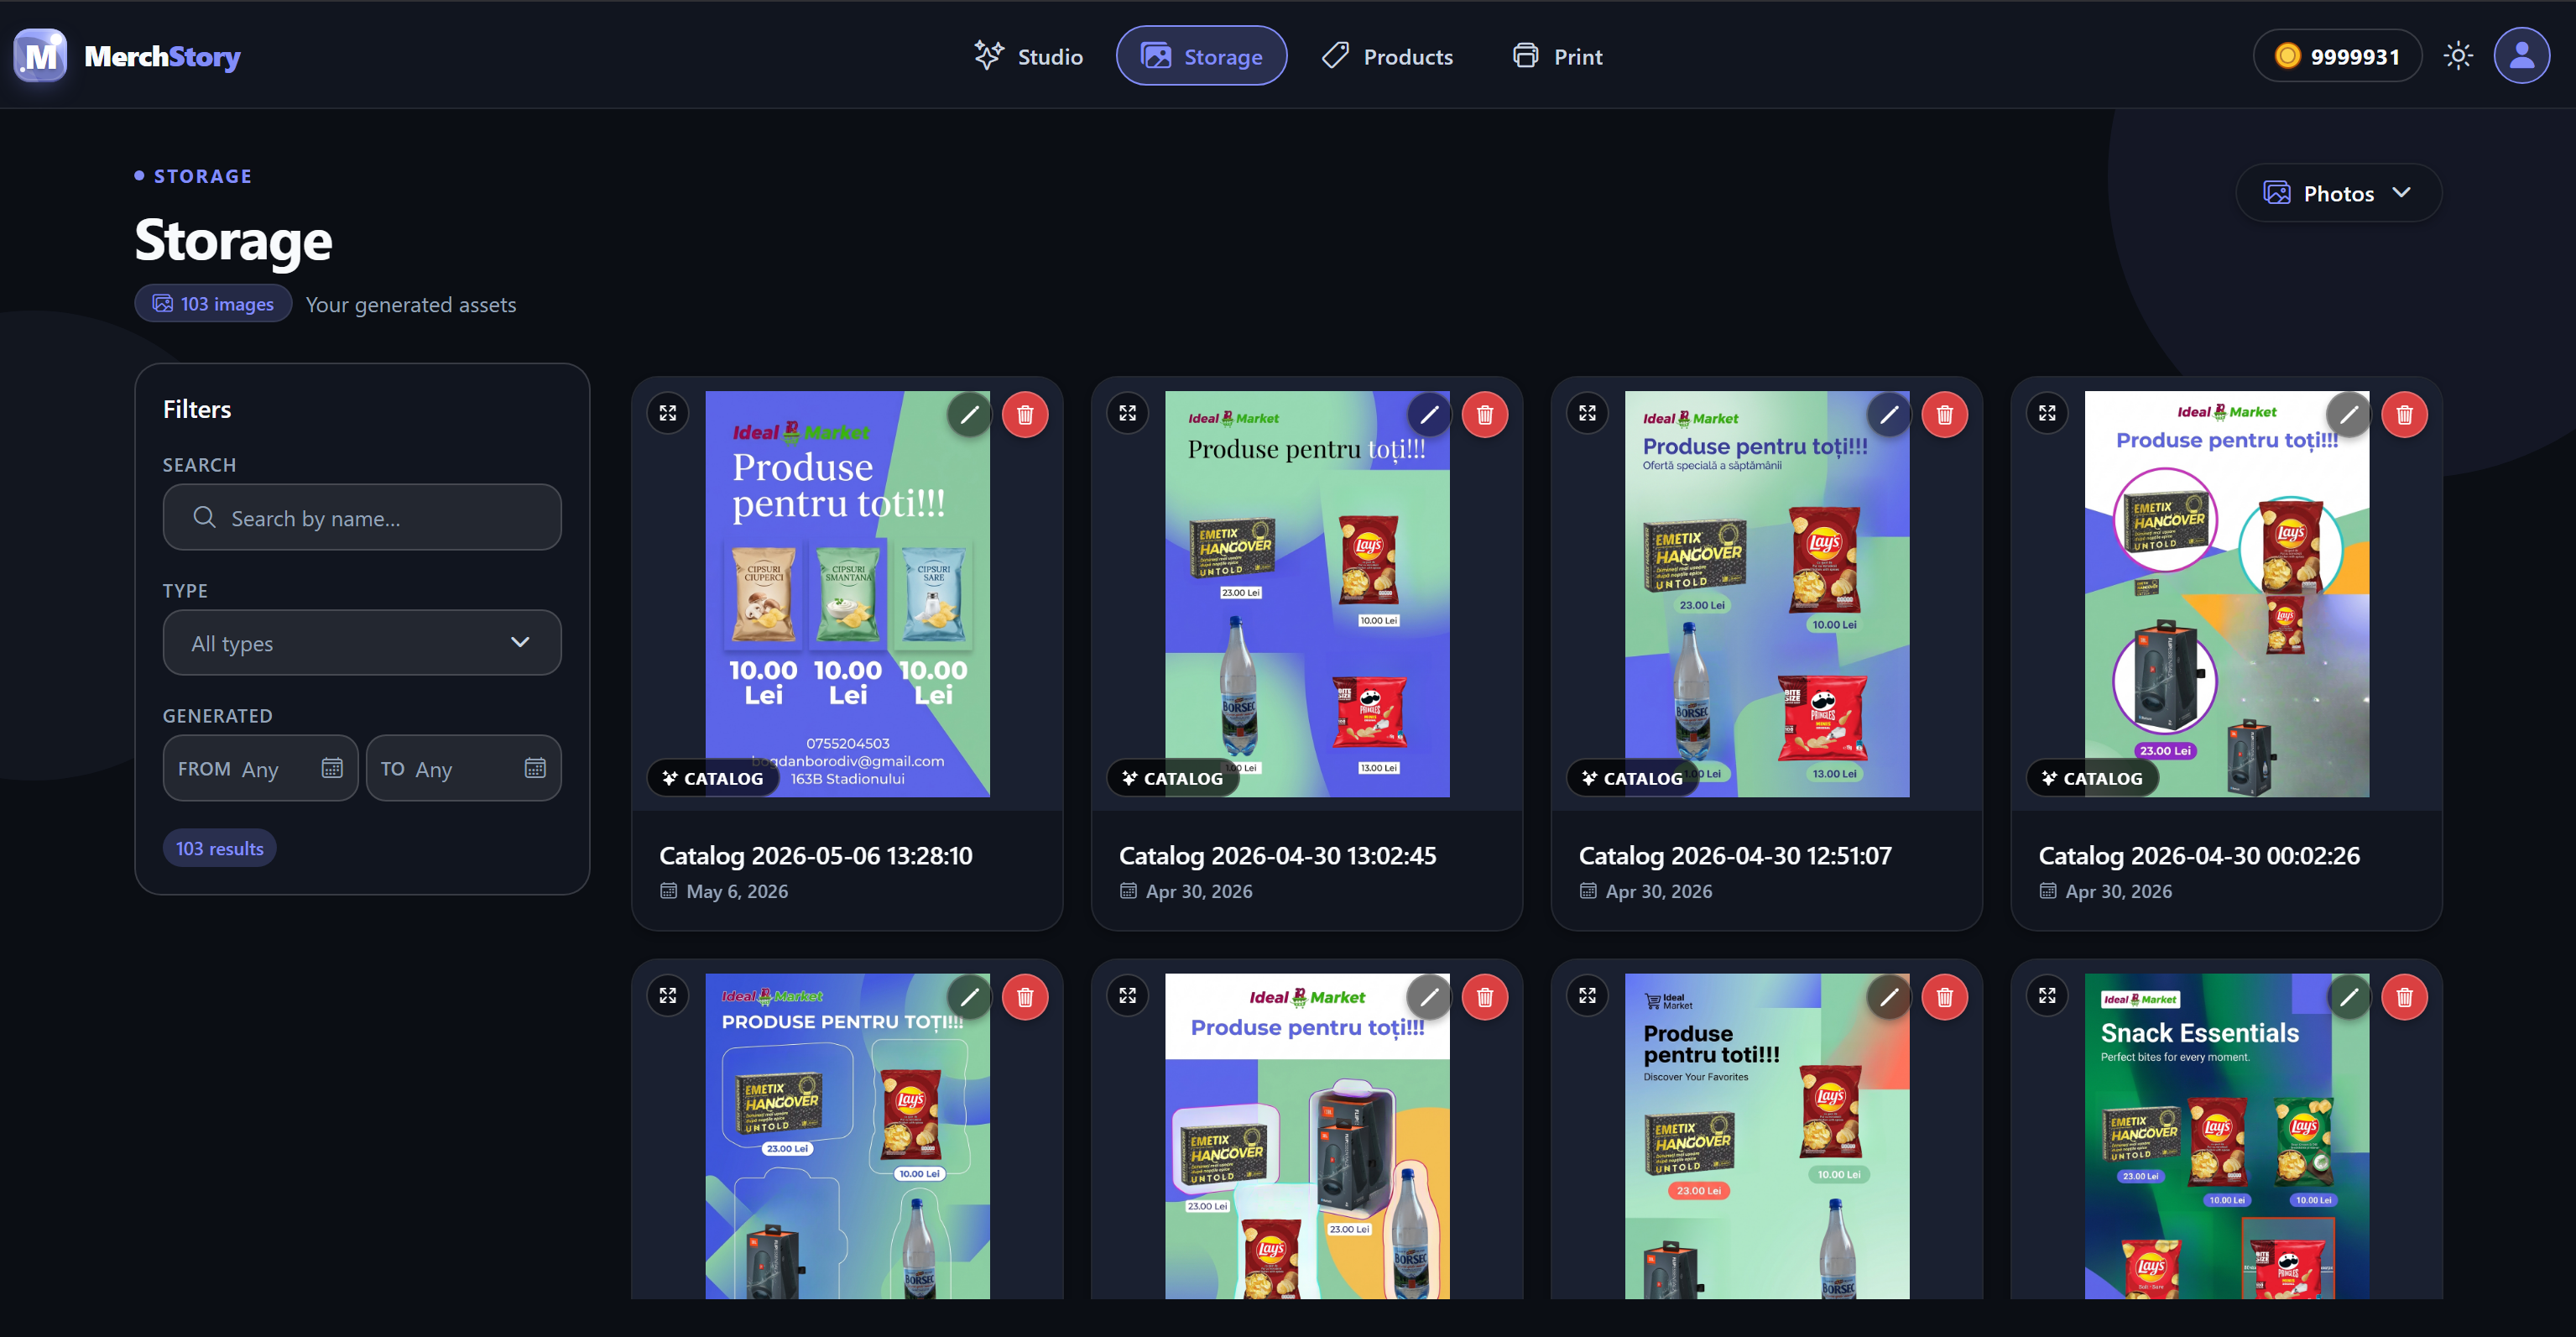
\includegraphics[width=\linewidth]{figures/client/gallery.png}
\end{minipage}\hfill
\begin{minipage}[t]{0.48\textwidth}
\centering
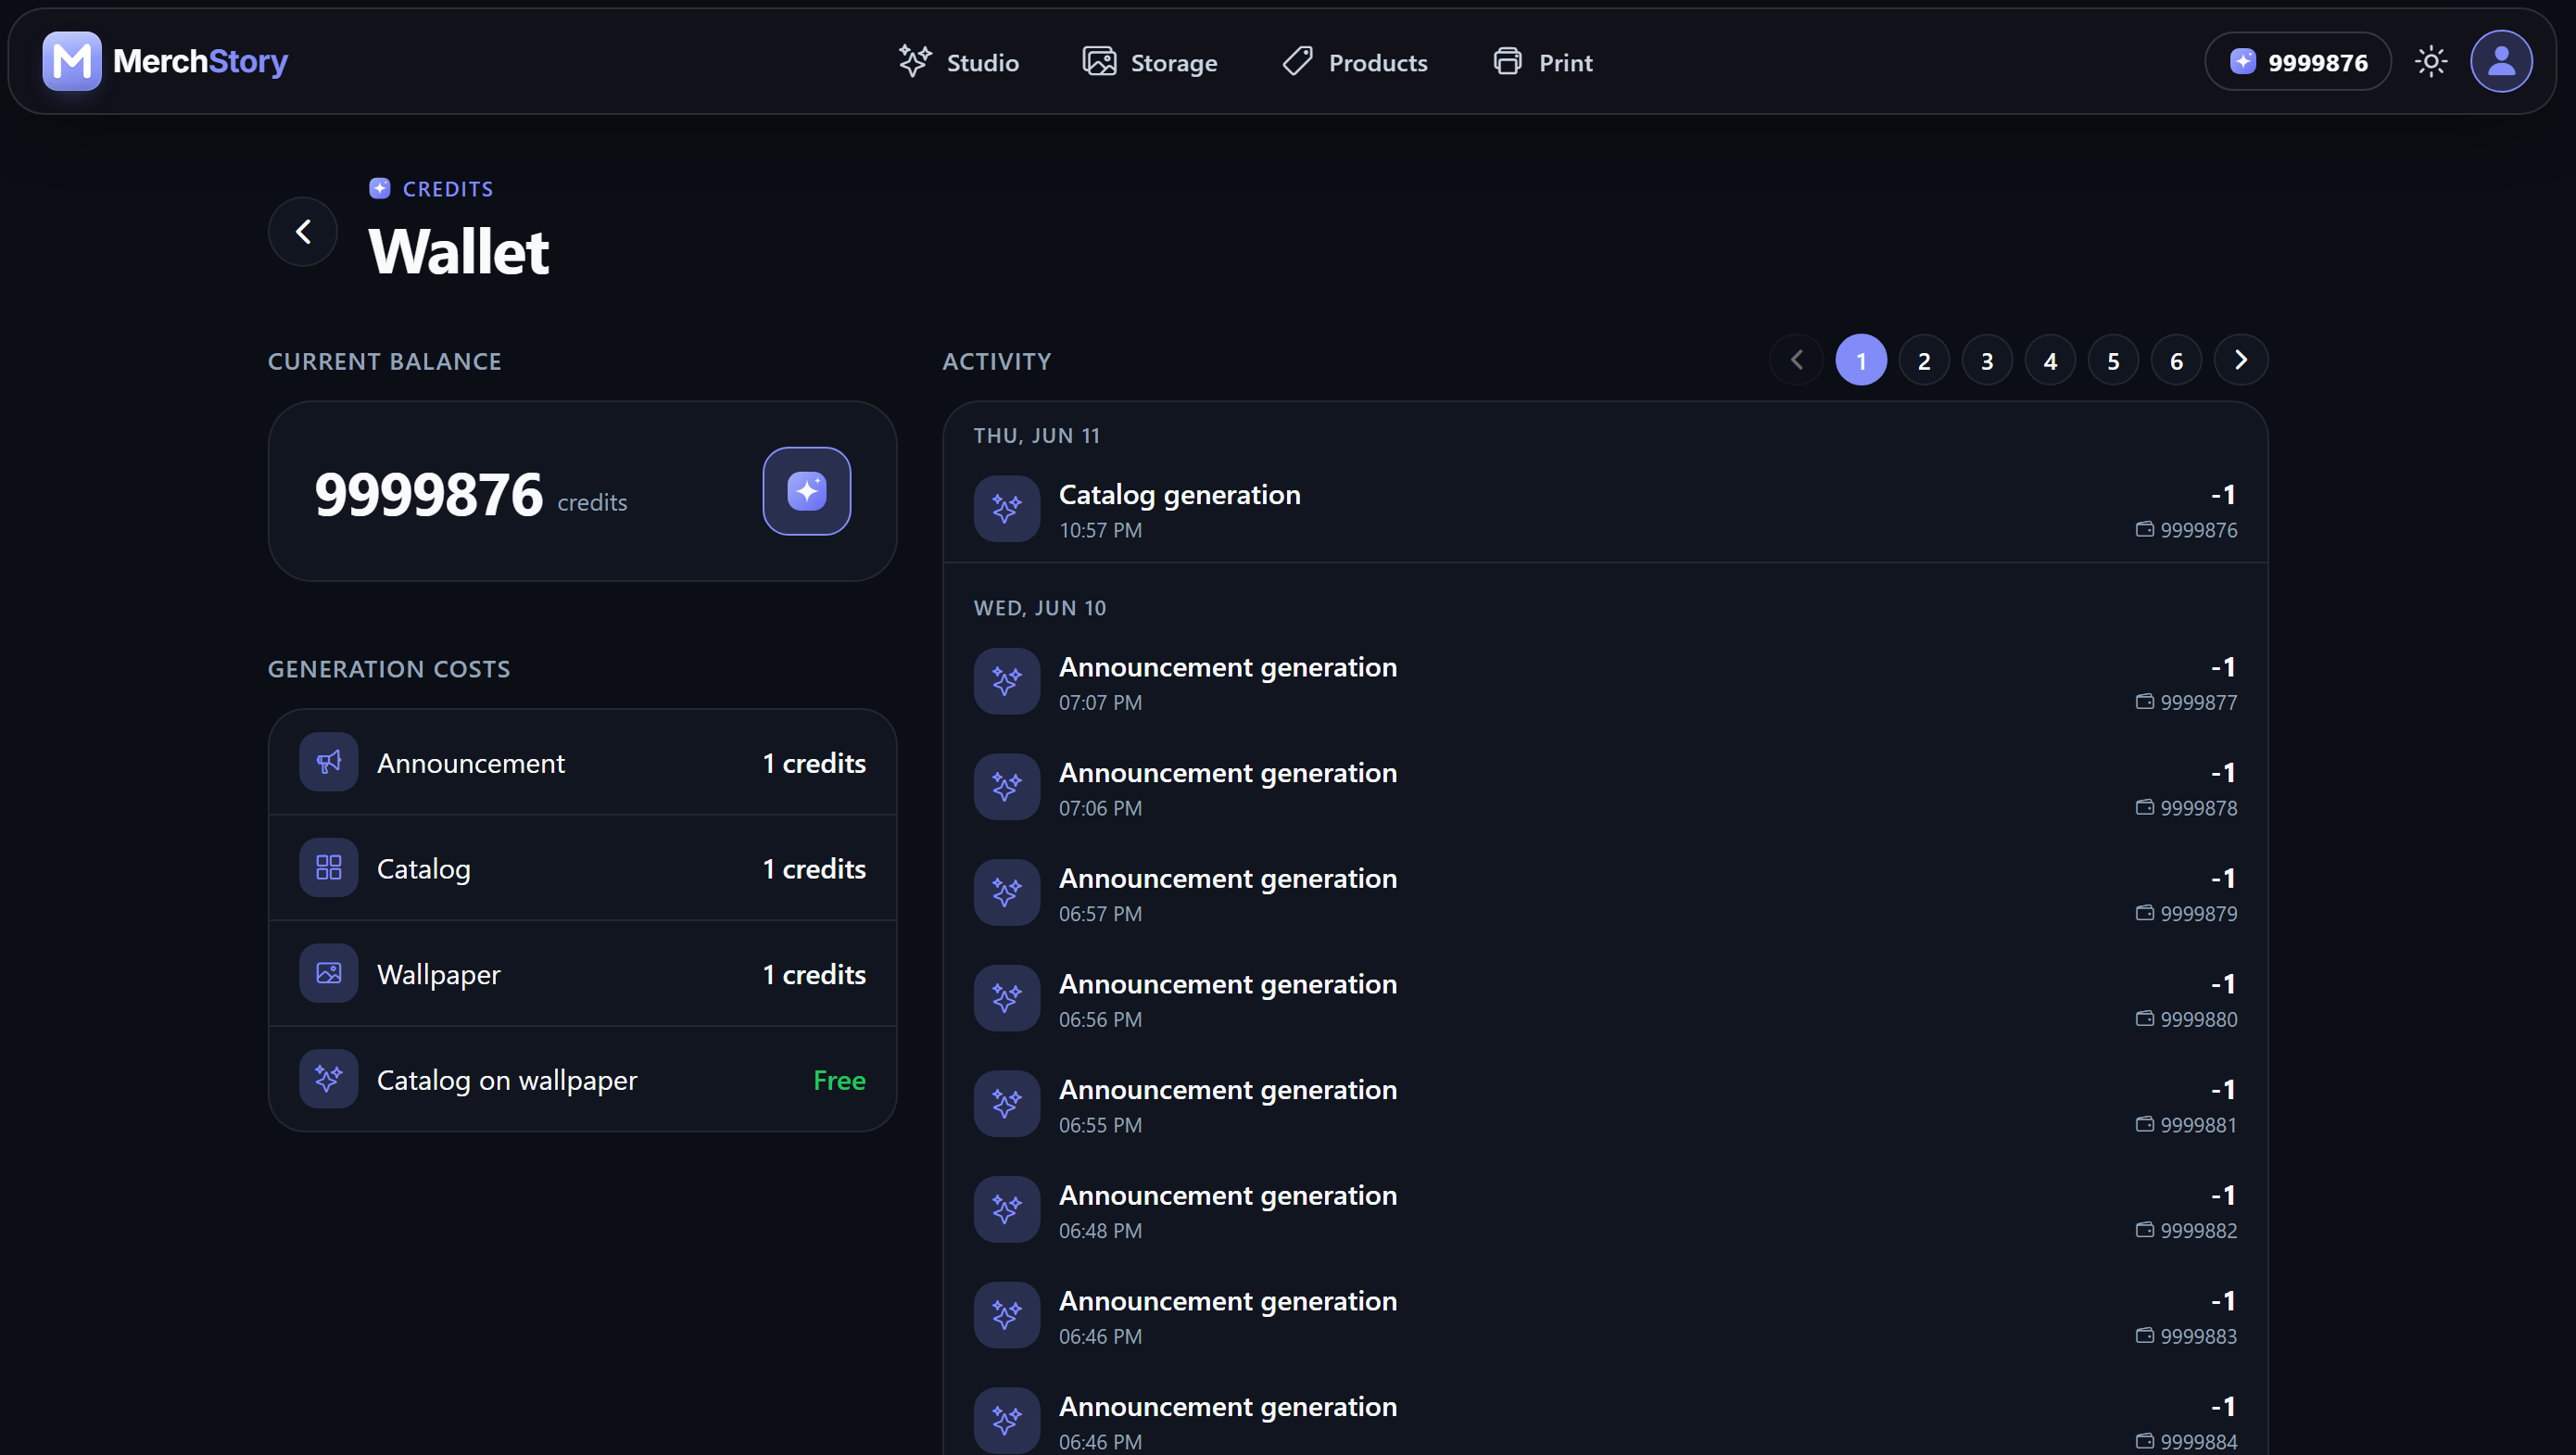
\includegraphics[width=\linewidth]{figures/client/wallet.png}
\end{minipage}
\caption{Gallery and wallet screens.}
\label{fig:client-output}
\end{figure}

\section{Application Server}
\label{sec:application-server}

The application server is a minimal-API ASP.NET Core service running on .NET 10. It hosts every feature service the platform exposes. It also hosts the two provider abstractions that AI calls pass through before they leave the server. Semantic Kernel handles the language-model work, and \textbf{IImageProvider} handles image generation.

\subsection{Stack choice, capability areas and internal layering}
\label{subsec:why-dotnet}

The choice of platform deserves comment because .NET is a less obvious pick for a contemporary AI application than Node.js or Python. One important part of the platform is a layer that orchestrates language-model calls. It routes prompts to several model backends, manages prompt templates, adds retrieval-augmented context to those calls, and runs several calls in a row for the daily recommendation engine. Microsoft's \emph{Semantic Kernel} \cite{semantickernel} is a first-class .NET library that bundles all of these facilities behind a unified abstraction, with clean integration into the ASP.NET Core dependency-injection container. Building the server in .NET therefore makes Semantic Kernel a native citizen of the architecture rather than a foreign component, which is the decisive reason for choosing ASP.NET Core minimal-API over Node.js with Express or Python with FastAPI.

Choosing Semantic Kernel does not tie the platform to one model vendor. The recommendation pipeline can run on local open-weight models through LM Studio or Ollama, on hosted DeepSeek or on OpenAI, and switching between them is a configuration change. Image generation does not use Semantic Kernel at all. It sits behind a separate interface called \textbf{IImageProvider}. In production this interface calls Google's Gemini image model, and it can also call OpenAI's GPT Image 2 model through the same interface. The image model can be changed from inside the platform, with no code change. Figure~\ref{fig:semantic-kernel} shows this arrangement.

\begin{figure}[!ht]
\centering
% --- same palette as Figure \ref{fig:three-tier} ---
\definecolor{cInk}{HTML}{2E3440}    % text + arrows
\definecolor{cIndigo}{HTML}{3F4D8C} % abstraction layers
\definecolor{cSlate}{HTML}{4A5568}  % application server
\definecolor{cGray}{HTML}{7C8390}   % backends
\resizebox{\textwidth}{!}{%
\begin{tikzpicture}[
    font=\sffamily\scriptsize,
    bar/.style={draw=#1, line width=0.9pt, rounded corners=3pt, align=center,
                text=cInk, drop shadow={shadow xshift=0.5mm, shadow yshift=-0.5mm,
                                        fill=black, opacity=0.12}},
    groupcard/.style={draw=#1, line width=0.9pt, rounded corners=3pt, inner sep=0pt,
                      dash pattern=on 2.4pt off 1.7pt, fill=#1!6},
    tab/.style={fill=#1, rounded corners=2.5pt, inner xsep=6pt, inner ysep=0pt,
                minimum height=5.2mm, anchor=south west,
                font=\sffamily\scriptsize\bfseries, text=white},
    chip/.style={draw=#1, line width=0.6pt, rounded corners=2.5pt, fill=white,
                 minimum height=9mm, align=center, text=cInk},
    arr/.style={-{Latex[length=2mm,width=1.5mm]}, line width=0.7pt, draw=cInk!85}
]

% ============ application server (top, full width) ============
\node[bar=cSlate, fill=cSlate!8, minimum width=150mm, minimum height=10mm]
      (api) at (0,5.0) {\textbf{Application server} \quad (ASP.NET Core, .NET 10)};

% ============ abstraction bars ============
\node[bar=cIndigo, fill=cIndigo!14, minimum width=84mm, minimum height=13mm]
      (sk) at (-3.3,3.0)
      {\textbf{Semantic Kernel}\\prompt templates \;$\cdot$\; retrieval-augmented context \;$\cdot$\; multi-stage chaining};
\node[bar=cIndigo, fill=cIndigo!14, minimum width=56mm, minimum height=13mm]
      (iface) at (4.5,3.0)
      {\textbf{IImageProvider}\\image generation};

% ============ backend group cards ============
\node[groupcard=cGray, minimum width=84mm, minimum height=28.5mm] (llmCard) at (-3.3,-0.03) {};
\node[groupcard=cGray, minimum width=56mm, minimum height=28.5mm] (imgCard) at ( 4.5,-0.03) {};

% ============ language-model backend chips ============
\node[chip=cGray, minimum width=38mm] (loc) at (-5.4, 0.65) {Local\\(LM Studio / Ollama)};
\node[chip=cGray, minimum width=28mm] (ds)  at (-1.7, 0.65) {DeepSeek};
\node[chip=cGray, minimum width=28mm] (oa)  at (-3.55,-0.70) {OpenAI};

% ============ image-generation backend chips ============
\node[chip=cGray, minimum width=50mm] (gem) at (4.5, 0.65) {Google Gemini};
\node[chip=cGray, minimum width=50mm] (gpt) at (4.5,-0.70) {GPT Image 2};

% ============ arrows ============
\draw[arr] (api.south) -- (sk.north);
\draw[arr] (api.south) -- (iface.north);
\draw[arr] (sk.south)    -- (llmCard.north);
\draw[arr] (iface.south) -- (imgCard.north);

% ============ group tabs (drawn last so they sit above the arrows) ============
\node[tab=cIndigo] at ([xshift=4mm]llmCard.north west) {Language-model backends};
\node[tab=cIndigo] at ([xshift=4mm]imgCard.north west) {Image-generation backends};

\end{tikzpicture}%
}
\caption{Provider abstractions on the application server.}
\label{fig:semantic-kernel}
\end{figure}

\label{subsec:capabilities}
Each capability area on the server is a bounded service that exposes a small set of HTTP endpoints. Authentication is handled inside the server itself: a successful login produces a short-lived JWT access token and a longer-lived refresh token. The access token is validated locally on every request, the refresh token is stored in the database and is rotated each time it is used, and a background service periodically removes tokens that have expired or been revoked.

The retailer-facing entities (shop profile, products, gallery, wallet) are each served by a dedicated feature service that exposes CRUD operations over its part of the schema, with the isolation rules inherited from the data layer. Coordination between services is performed at the endpoint layer rather than through direct inter-service calls.

A thin orchestration layer fronts the supported image providers behind a single \textbf{IImageProvider} abstraction shown in Listing~\ref{lst:iimageprovider}. Each provider has a concrete implementation that wraps its SDK, and a mock implementation returns a deterministic placeholder image during automated testing.

\begin{lstlisting}[style=csharp, caption={The IImageProvider abstraction.}, label={lst:iimageprovider}]
public interface IImageProvider
{
    Task<ImageGenerationResult> GenerateAsync(
        string prompt,
        IReadOnlyList<string?>? inlineImages = null,
        CancellationToken cancellationToken = default);
}
\end{lstlisting}

The daily recommendation engine is exposed as its own service, whose inputs and outputs match the functional requirement above and whose internals are the subject of the contributions chapter that follows. Sitting alongside it is the credit ledger, an in-process service that mediates between every billable AI call and the database. The ledger exposes a single primitive, \emph{run-with-debit}, which opens a database transaction, debits the cost, runs the work, and commits only when the work succeeds. A failure rolls the transaction back so that no debit is ever recorded for unsuccessful work.

Two long-running background services run in the same process as the request handler: a job runner that consumes pending recommendation runs, and a cleaner that deletes expired refresh tokens. At the platform's data volumes a separate worker tier is not justified. All of this is exposed over a small, feature-grouped HTTP API; Table~\ref{tab:http-endpoints} lists each route group along with its prefix and purpose.

{\small
\renewcommand{\arraystretch}{1.3}
\begin{tabularx}{\textwidth}{|>{\raggedright\arraybackslash}p{3.2cm}|>{\raggedright\arraybackslash}p{3.6cm}|Y|}
\caption{HTTP route groups exposed by the application server.}\label{tab:http-endpoints}\\
\hline
\textbf{Group} & \textbf{Prefix} & \textbf{Purpose} \\
\hline
\endfirsthead
\hline
\textbf{Group} & \textbf{Prefix} & \textbf{Purpose} \\
\hline
\endhead
\hline
\endfoot
\hline
\endlastfoot
Auth & /auth & Register, log in, refresh tokens and change interface language. \\
\hline
Shop & /shop & Read and update the shop profile and logo. \\
\hline
Products & /products & CRUD over the retailer's product library, with one-tap background removal. \\
\hline
Reference catalogue & /reference-images & Browse, search and bulk-import the curated reference catalogue. \\
\hline
Image generation & /generate-image & Produce announcements, catalogues and wallpapers in fully generative or hybrid mode. \\
\hline
Gallery & /gallery & Save, list, rename and delete generated assets. \\
\hline
Wallet & /wallet & Read the credit balance and ledger, and grant credits (operator only). \\
\hline
Recommendations & /recommendations & Fetch today's ideas, request a refresh and leave feedback. \\
\hline
Print & /print & Render a gallery item to a print-ready document. \\
\end{tabularx}
}

\paragraph{Internal layering.}\label{subsec:server-layering}
Each feature follows a simple internal layering, shown in Figure~\ref{fig:server-layering}. The endpoint layer handles HTTP concerns only and delegates to a feature service that holds the business logic. The feature service then calls the data layer. For AI work it instead calls one of the provider abstractions, which are Semantic Kernel for language-model calls and \textbf{IImageProvider} for image generation. Those abstractions are the only place from which outbound HTTP calls to third parties leave, which keeps retries, circuit breakers and credential management in one place.

\begin{figure}[H]
\centering
% --- same palette as Figure \ref{fig:three-tier} ---
\definecolor{cInk}{HTML}{2E3440}    % text + arrows
\definecolor{cIndigo}{HTML}{3F4D8C} % entry / orchestration
\definecolor{cSlate}{HTML}{4A5568}  % feature internals
\definecolor{cGray}{HTML}{7C8390}   % external boundary
\begin{tikzpicture}[
    font=\sffamily\scriptsize,
    bar/.style={draw=#1, line width=0.9pt, rounded corners=3pt, align=center,
                minimum width=90mm, minimum height=13mm, text=cInk,
                drop shadow={shadow xshift=0.5mm, shadow yshift=-0.5mm,
                             fill=black, opacity=0.12}},
    extbar/.style={draw=cGray, line width=0.9pt, rounded corners=3pt, align=center,
                   dash pattern=on 2.4pt off 1.7pt, fill=cGray!6,
                   minimum width=90mm, minimum height=13mm, text=cInk},
    arr/.style={-{Latex[length=2mm,width=1.5mm]}, line width=0.7pt, draw=cInk!85}
]
\node[bar=cIndigo, fill=cIndigo!7]  (ep)   at (0,0)
      {\textbf{Endpoints}\\HTTP concerns only \;$\cdot$\; \texttt{Map\dots Endpoints}};
\node[bar=cSlate,  fill=cSlate!8]   (svc)  at (0,-2.0)
      {\textbf{Feature services}\\business logic for one feature};
\node[bar=cIndigo, fill=cIndigo!14] (orch) at (0,-4.0)
      {\textbf{Provider abstractions}\\Semantic Kernel \;$\cdot$\; \textbf{IImageProvider}};
\node[extbar]                       (http) at (0,-6.0)
      {\textbf{External HTTP boundary}\\outbound third-party calls leave here};
\draw[arr] (ep)   -- (svc);
\draw[arr] (svc)  -- (orch);
\draw[arr] (orch) -- (http);
\end{tikzpicture}
\caption{Internal layering of a feature folder on the server.}
\label{fig:server-layering}
\end{figure}

\section{Data Layer}
\label{sec:data-layer}

The data layer holds every piece of state that survives a request. PostgreSQL with the pgvector extension stores all relational data and the platform's two embedding spaces, and a separate Azure Blob Storage account holds the binary assets. Figure~\ref{fig:data-plane} shows the arrangement and the Azure-hosted compute that reads and writes it.

\begin{figure}[H]
\centering
% --- same palette as Figure \ref{fig:three-tier} ---
\definecolor{cInk}{HTML}{2E3440}    % text + arrows
\definecolor{cSlate}{HTML}{4A5568}  % Azure compute
\definecolor{cTeal}{HTML}{2E5F8C}   % data plane
\resizebox{\textwidth}{!}{%
\begin{tikzpicture}[
    font=\sffamily\scriptsize,
    card/.style={draw=#1, line width=0.9pt, rounded corners=3pt, inner sep=0pt,
                 drop shadow={shadow xshift=0.5mm, shadow yshift=-0.5mm,
                              fill=black, opacity=0.12}},
    tab/.style={fill=#1, rounded corners=2.5pt, inner xsep=6pt, inner ysep=0pt,
                minimum height=5.2mm, anchor=south west,
                font=\sffamily\scriptsize\bfseries, text=white},
    chip/.style={draw=#1, line width=0.6pt, rounded corners=2.5pt, fill=white,
                 minimum width=32mm, minimum height=11mm, align=center, text=cInk},
    store/.style={draw=cTeal, line width=0.6pt, cylinder, shape border rotate=90,
                  aspect=0.22, minimum width=27mm, minimum height=16mm, align=center,
                  cylinder uses custom fill, cylinder body fill=white,
                  cylinder end fill=cTeal!15, text=cInk},
    arr/.style={-{Latex[length=2mm,width=1.5mm]}, line width=0.7pt, draw=cInk!85}
]

% ============ cards (drawn first, content on top) ============
\node[card=cSlate, fill=cSlate!8, minimum width=118mm, minimum height=19mm]
      (computeCard) at (0,3.2) {};
\node[card=cTeal, fill=cTeal!8, minimum width=92mm, minimum height=21mm]
      (pgCard) at (-1.4,0) {};

% ============ compute chips ============
\node[chip=cSlate] (api)    at (-3.9,3.2) {API replicas\\(.NET 10)};
\node[chip=cSlate] (recjob) at (0,3.2)    {Recommendation\\job runner};
\node[chip=cSlate] (tokjob) at (3.9,3.2)  {Refresh-token\\cleaner};

% ============ database sub-stores ============
\node[chip=cTeal, minimum width=26mm, minimum height=14mm] (relt) at (-4.2,0)
      {Relational\\tables};
\node[chip=cTeal, minimum width=26mm, minimum height=14mm] (clip) at (-1.4,0)
      {pgvector\\(CLIP image\\embeddings)};
\node[chip=cTeal, minimum width=26mm, minimum height=14mm] (txt)  at (1.4,0)
      {pgvector\\(text\\embeddings)};

% ============ blob storage ============
\node[store] (blobstore) at (4.9,0) {Azure\\Blob Storage};

% ============ arrows ============
\draw[arr] (computeCard.south -| 1.9,0) -- (pgCard.north -| 1.9,0);
\draw[arr] (computeCard.south -| blobstore.north) -- (blobstore.north);

% ============ card header tabs (drawn last) ============
\node[tab=cSlate] at ([xshift=4mm]computeCard.north west) {Azure Container Apps revision};
\node[tab=cTeal]  at ([xshift=4mm]pgCard.north west) {Azure Database for PostgreSQL Flexible Server};

\end{tikzpicture}%
}
\caption{The data plane and the Azure compute that reads and writes it.}
\label{fig:data-plane}
\end{figure}

\subsection{Relational schema, caching and object storage}
\label{subsec:relational-schema}

The schema is a foreign-key spine that ties every record to a tenant. At its centre is the user-account table, with one row per retailer and a flag for operators. The other tables fall into two groups: tenant-scoped tables that hang off the user, and global tables that hold catalogue data and context signals shared across tenants. Figure~\ref{fig:schema} shows the arrangement.

\begin{figure}[H]
\centering
% --- same palette as Figure \ref{fig:three-tier} ---
\definecolor{cInk}{HTML}{2E3440}    % text + arrows
\definecolor{cIndigo}{HTML}{3F4D8C} % AppUser hub
\definecolor{cSlate}{HTML}{4A5568}  % plain entities
\definecolor{cTeal}{HTML}{2E5F8C}   % vector-bearing entities + data plane
\resizebox{\textwidth}{!}{%
\begin{tikzpicture}[
    font=\sffamily\scriptsize,
    ent/.style={rectangle split, rectangle split parts=2,
                rectangle split part fill={#1, white},
                draw=#1, line width=0.6pt, rounded corners=2pt,
                text width=27mm, align=left, inner sep=3pt, text=cInk},
    card/.style={draw=#1, line width=0.9pt, rounded corners=3pt, fill=#1!6,
                 drop shadow={shadow xshift=0.5mm, shadow yshift=-0.5mm,
                              fill=black, opacity=0.12}},
    tab/.style={fill=#1, rounded corners=2.5pt, inner xsep=6pt, inner ysep=0pt,
                minimum height=5.2mm, anchor=south west,
                font=\sffamily\scriptsize\bfseries, text=white},
    fk/.style={-{Latex[length=2mm,width=1.5mm]}, line width=0.7pt, draw=cInk!85}
]

% ============ tenant-scoped tables above AppUser ============
\node[ent=cSlate, anchor=south] (shop) at (-5.6, 3.2) {%
    \textcolor{white}{\bfseries ShopProfile}
    \nodepart{two}
    UserId (FK, unique)\\
    BrandName\\
    BusinessDomain\\
    Currency
};
\node[ent=cSlate, anchor=south] (prod) at (0, 3.2) {%
    \textcolor{white}{\bfseries Product}
    \nodepart{two}
    UserId (FK)\\
    Name\\
    Price, Category\\
    ImageBlobKey
};
\node[ent=cSlate, anchor=south] (gen) at (5.6, 3.2) {%
    \textcolor{white}{\bfseries GeneratedImage}
    \nodepart{two}
    UserId (FK)\\
    Name\\
    AssetType\\
    ImageBlobKey
};

% ============ AppUser at centre ============
\node[ent=cIndigo, line width=0.9pt] (user) at (0, 1.5) {%
    \textcolor{white}{\bfseries AppUser}
    \nodepart{two}
    Id (PK)\\
    Email\\
    IsAdmin\\
    CreditBalance
};

% ============ tenant-scoped tables below AppUser ============
\node[ent=cSlate, anchor=north] (coin) at (-5.6,-0.2) {%
    \textcolor{white}{\bfseries CreditTransaction}
    \nodepart{two}
    UserId (FK)\\
    Amount\\
    BalanceAfter\\
    RelatedGenImage (FK)
};
\node[ent=cSlate, anchor=north] (rec) at (0,-0.2) {%
    \textcolor{white}{\bfseries DailyRecommend.}
    \nodepart{two}
    UserId (FK)\\
    GeneratedAtUtc\\
    IdeasJson
};
\node[ent=cTeal, anchor=north] (emb) at (5.6,-0.2) {%
    \textcolor{white}{\bfseries IdeaEmbedding}
    \nodepart{two}
    UserId (FK)\\
    DailyRecId (FK)\\
    Embedding (text)
};

% ============ FK arrows tenant -> AppUser ============
\draw[fk] (shop) -- (user);
\draw[fk] (prod) -- (user);
\draw[fk] (gen)  -- (user);
\draw[fk] (coin) -- (user);
\draw[fk] (rec)  -- (user);
\draw[fk] (emb)  -- (user);

% ============ global tables ============
\node[ent=cSlate, anchor=north] (cat) at (-6.9,-5.0) {%
    \textcolor{white}{\bfseries Category}
    \nodepart{two}
    Id (PK)\\
    Name\\
    ParentCategoryId (FK self)
};
\node[ent=cTeal, anchor=north] (rim) at (-2.3,-5.0) {%
    \textcolor{white}{\bfseries ReferenceImage}
    \nodepart{two}
    CategoryId (FK)\\
    Name\\
    ImageBlobKey\\
    Embedding (CLIP)
};
\node[ent=cTeal, anchor=north] (pp) at (2.3,-5.0) {%
    \textcolor{white}{\bfseries PromoPlaybook}
    \nodepart{two}
    BusinessDomain\\
    Theme, Trigger\\
    Tactics\\
    Embedding (text)
};
\node[ent=cSlate, anchor=north] (hol) at (6.9,-5.0) {%
    \textcolor{white}{\bfseries Holiday}
    \nodepart{two}
    CountryCode\\
    Year, Date\\
    Name
};

\draw[fk] (rim) -- (cat);
\draw[fk] (cat.north) .. controls +(125:9mm) and +(55:9mm) .. (cat.north);

% phantom apex so the global card encloses the self-loop
\node[inner sep=0pt, minimum size=0pt] (catloop) at (-6.9,-4.25) {};

% ============ group cards (background) ============
\begin{pgfonlayer}{background}
\node[card=cTeal, inner sep=4mm, minimum width=174mm,
      fit=(shop)(prod)(gen)(user)(coin)(rec)(emb)] (tenantCard) {};
\node[card=cTeal, inner sep=3mm, minimum width=174mm,
      fit=(cat)(rim)(pp)(hol)(catloop)] (globalCard) {};
\end{pgfonlayer}

% ============ card header tabs (drawn last) ============
\node[tab=cTeal] at ([xshift=4mm]tenantCard.north west) {Tenant-scoped tables};
\node[tab=cTeal] at ([xshift=4mm]globalCard.north west) {Global tables};

\end{tikzpicture}%
}
\caption{Database schema with key fields.}
\label{fig:schema}
\end{figure}

Two consequences of this layout matter at runtime. The first is that tenant isolation is enforced at the schema level rather than relying on application discipline. Every retailer-owned row carries a UserId foreign key, and the feature services filter on it before returning any data, so a misbehaving or malformed query can at worst read the wrong row, never the wrong tenant's data. The second is that the credit ledger is append-only and self-checking. Each CreditTransaction stores the delta and the resulting balance, so the wallet can be reconciled against the ledger at any point and a divergence would surface immediately. Together these properties hand the schema responsibility for two of the platform's hardest invariants, which would otherwise be re-verified by every endpoint touching retailer data or money.

{\footnotesize
\renewcommand{\arraystretch}{1.1}
\begin{tabularx}{\textwidth}{|>{\raggedright\arraybackslash}p{4.5cm}|Y|}
\caption{Purpose of each table in the schema.}\label{tab:schema-tables}\\
\hline
\textbf{Table} & \textbf{Purpose} \\
\hline
\endfirsthead
\hline
\textbf{Table} & \textbf{Purpose} \\
\hline
\endhead
\hline
\endfoot
\hline
\endlastfoot
AppUser & Identifies a retailer (or operator) and tracks the credit balance. \\
\hline
ShopProfile & Holds the brand identity and contact details captured during onboarding. \\
\hline
Product & An item the retailer sells, with name, price and a representative photograph. \\
\hline
GeneratedImage & An entry in the gallery, tagged with its asset family. \\
\hline
CreditTransaction & A row of the credit ledger that records a debit or refund and, optionally, the asset it paid for. \\
\hline
DailyRecommendation & The day's marketing ideas together with the context snapshot used to produce them. \\
\hline
IdeaEmbedding & A per-idea text embedding used to deduplicate themes against the shop's recent ideas. \\
\hline\hline
Category & A node in the reference catalogue's hierarchical tree. \\
\hline
ReferenceImage & A curated product photograph with a CLIP embedding for search-by-photo. \\
\hline
PromoPlaybookEntry & A known-good promotional pattern with a text embedding the recommendation engine retrieves over. \\
\hline
Holiday & A cached public holiday for a country and year, used as a context signal. \\
\end{tabularx}
}

\paragraph{Caching.}\label{subsec:caching}
A few screens show the same data every time the retailer opens them, such as the product list and the gallery. To make these screens feel fast, the client keeps a small cache on the device for the product list and the gallery. When the retailer adds, edits or removes something, the client clears the matching entry, so the next read fetches fresh data from the server. The cache lives on the device and not on the server, so the platform does not need a separate cache service.

\paragraph{Object storage.}\label{subsec:object-storage}
Binary assets such as raw and processed product photographs, generated images and exported PDFs are kept out of the relational database and live in Microsoft Azure Blob Storage. The arrangement is conventional and is justified by the cost asymmetry between row storage and blob storage, and by the need to serve large files efficiently. The relational schema records the blob key and content type for each binary, and access is mediated by short-lived signed URLs (SAS tokens) issued by the application server, so that no public URL ever leaks beyond the request that needs it. Containers are private with no anonymous access tier, and the only path through which a retailer's assets are reachable is the application server.

\begin{figure}[!ht]
\centering
% --- same palette as Figure \ref{fig:three-tier} ---
\definecolor{cInk}{HTML}{2E3440}    % text + arrows
\definecolor{cIndigo}{HTML}{3F4D8C} % client
\definecolor{cSlate}{HTML}{4A5568}  % application server
\definecolor{cTeal}{HTML}{2E5F8C}   % data stores
\definecolor{cAmber}{HTML}{B07A1F}  % signing step
\resizebox{\textwidth}{!}{%
\begin{tikzpicture}[
    font=\sffamily\scriptsize,
    actor/.style={draw=#1, line width=0.6pt, rounded corners=2.5pt, fill=white,
                  minimum width=27mm, minimum height=7.5mm, align=center, text=cInk},
    life/.style={draw=cInk!35, line width=0.6pt, dash pattern=on 2.4pt off 1.7pt},
    arr/.style={-{Latex[length=2mm,width=1.5mm]}, line width=0.7pt, draw=cInk!85},
    every node/.style={text=cInk}
]

% ============ actors ============
\node[actor=cIndigo] (client) at (0, 5)   {Client};
\node[actor=cSlate]  (server) at (4.5, 5) {Application server};
\node[actor=cTeal]   (db)     at (9, 5)   {PostgreSQL};
\node[actor=cTeal]   (blob)   at (13, 5)  {Blob storage};

% ============ lifelines ============
\draw[life] (client.south) -- (0,-1.6);
\draw[life] (server.south) -- (4.5,-1.6);
\draw[life] (db.south)     -- (9,-1.6);
\draw[life] (blob.south)   -- (13,-1.6);

% ============ messages ============
\draw[arr] (0, 4.0)   -- node[above]{1. GET image} (4.5, 4.0);
\draw[arr] (4.5, 3.2) -- node[above]{2. lookup blob key} (9, 3.2);
\draw[arr] (9, 2.4)   -- node[above]{3. blob key + content type} (4.5, 2.4);
\node[draw=cAmber, line width=0.6pt, rounded corners=2.5pt, fill=cAmber!12,
      inner xsep=5pt, inner ysep=3pt] at (4.5, 1.6) {\itshape sign SAS URL};
\draw[arr] (4.5, 0.8) -- node[above]{4. signed SAS URL} (0, 0.8);
\draw[arr] (0, -0.2)  -- node[above]{5. GET via signed URL} (13, -0.2);
\draw[arr] (13, -1.0) -- node[above]{6. image bytes} (0, -1.0);

\end{tikzpicture}%
}
\caption{Image retrieval flow.}
\label{fig:object-storage-flow}
\end{figure}

\section{Cloud Deployment on Microsoft Azure}
\label{sec:azure-deployment}

Azure was chosen because it gives the platform a managed, well-supported and trustworthy foundation for everything outside the AI calls themselves. The platform runs on .NET and uses Semantic Kernel for orchestration, both of which are Microsoft technologies and receive first-class support on Azure. Azure also brings enterprise-grade reliability, regional redundancy and a long track record of security and compliance certifications, all of which matter for a service that holds retailer data and runs paid AI calls on their behalf. The managed services Azure offers, from PostgreSQL Flexible Server to Container Apps, Key Vault, Blob Storage and Application Insights, fit the platform's needs without requiring a dedicated operations team.

\begin{figure}[ht]
\centering
% --- same palette as Figure \ref{fig:three-tier} ---
\definecolor{cInk}{HTML}{2E3440}    % text + arrows
\definecolor{cIndigo}{HTML}{3F4D8C} % client / ingress / VNet
\definecolor{cSlate}{HTML}{4A5568}  % Azure compute + ops
\definecolor{cTeal}{HTML}{2E5F8C}   % data + secrets
\definecolor{cGray}{HTML}{7C8390}   % external third-party
\resizebox{\textwidth}{!}{%
\begin{tikzpicture}[
    font=\sffamily\scriptsize,
    card/.style={draw=#1, line width=0.9pt, rounded corners=3pt, inner sep=0pt,
                 drop shadow={shadow xshift=0.5mm, shadow yshift=-0.5mm,
                              fill=black, opacity=0.12}},
    tab/.style={fill=#1, rounded corners=2.5pt, inner xsep=6pt, inner ysep=0pt,
                minimum height=5.2mm, anchor=south west,
                font=\sffamily\scriptsize\bfseries, text=white},
    chip/.style={draw=#1, line width=0.6pt, rounded corners=2.5pt, fill=white,
                 minimum width=30mm, minimum height=10mm, align=center, text=cInk},
    store/.style={draw=cTeal, line width=0.6pt, cylinder, shape border rotate=90,
                  aspect=0.22, minimum width=26mm, minimum height=15mm, align=center,
                  cylinder uses custom fill, cylinder body fill=white,
                  cylinder end fill=cTeal!15, text=cInk},
    ext/.style={draw=cGray, line width=0.6pt, dash pattern=on 2.4pt off 1.7pt,
                rounded corners=2.5pt, fill=white, minimum width=28mm,
                minimum height=10mm, align=center, text=cInk},
    arr/.style={-{Latex[length=2mm,width=1.5mm]}, line width=0.7pt, draw=cInk!85}
]

% ============ containers (drawn first, content on top) ============
\node[card=cIndigo, fill=cIndigo!6, minimum width=140mm, minimum height=61mm]
      (vnet) at (0,3.05) {};
\node[card=cSlate, fill=cSlate!8, minimum width=72mm, minimum height=17mm]
      (capps) at (-1.9,4.45) {};

% ============ top row: client and GitHub ============
\node[chip=cIndigo] (cl)     at (0.6,9.3) {Client\\(web, iOS, Android)};
\node[ext]          (github) at (4.8,9.3) {GitHub repo\\(Actions CI/CD)};

% ============ ingress (hero bar) ============
\node[draw=cIndigo, line width=0.9pt, rounded corners=3pt, fill=cIndigo!14,
      minimum width=50mm, minimum height=10mm, align=center, text=cInk,
      drop shadow={shadow xshift=0.5mm, shadow yshift=-0.5mm,
                   fill=black, opacity=0.12}]
      (apim) at (0.6,7.6) {Container Apps ingress\\(TLS, Azure DDoS)};

% ============ Container Apps Environment ============
\node[chip=cSlate] (api) at (-3.6,4.45) {\texttt{merchstory-api}};
\node[chip=cSlate] (web) at (-0.2,4.45) {\texttt{merchstory-web}};

% ============ registry ============
\node[chip=cSlate] (acr) at (4.8,4.45) {Container Registry\\(\texttt{merchstoryacr})};

% ============ data, secrets and ops row ============
\node[store]       (db)   at (-5.0,1.2) {PostgreSQL\\Flexible Server\\(pgvector)};
\node[store]       (blob) at (-1.6,1.2) {Azure\\Blob Storage};
\node[chip=cTeal]  (kv)   at (1.8,1.2)  {Azure Key Vault};
\node[chip=cSlate] (logs) at (5.0,1.2)  {App Insights\\+ Log Analytics};

% ============ external (non-Azure) services ============
\node[ext] (aip) at (-9.8,5.5) {Multimodal AI\\providers};
\node[ext] (bg)  at (-9.8,4.3) {Background\\removal};
\node[ext] (geo) at (-9.8,3.1) {Geocoding};

% ============ arrows ============
% client traffic
\draw[arr] (cl) -- (apim);
\draw[arr] (apim.south) -- (capps.north -| 0.6,0);
% CI/CD: GitHub push, ACR pull
\draw[arr] (github) -- node[right]{push image} (acr);
\draw[arr] (acr) -- node[above, xshift=2mm]{pull image} (web);
% api -> data plane
\draw[arr] (api) -- (db.north);
\draw[arr] (api) -- (blob.north);
\draw[arr] (api) -- (kv.north);
\draw[arr] (api) -- (logs.north);
% api -> external services
\draw[arr] (api.west) -- (aip.east);
\draw[arr] (api.west) -- (bg.east);
\draw[arr] (api.west) -- (geo.east);

% ============ container tabs (drawn last so they sit above the arrows) ============
\node[tab=cIndigo] at ([xshift=4mm]vnet.north west)  {private VNet};
\node[tab=cSlate]  at ([xshift=4mm]capps.north west) {Container Apps Environment};

\end{tikzpicture}%
}
\caption{The platform's deployment topology on Microsoft Azure.}
\label{fig:deployment}
\end{figure}

The application server runs on Azure Container Apps, a managed container runtime built on Kubernetes that provides per-replica scale-out without the operational burden of managing a cluster directly. The choice was made over Azure App Service on two grounds. First, the platform packages its server as a container image already. Second, Container Apps integrates more cleanly with Azure API Management and with the private virtual network in which the data plane lives. A single long-running background service, the refresh-token cleaner, runs inside the same Container Apps revision as the API. Recommendation generations are started by request handlers as fire-and-forget tasks tracked by an in-memory job registry, so a separate worker tier is not justified at the platform's data volumes. The web build of the client runs as its own Azure Container App (\texttt{merchstory-web}), pulling its image from the same registry as the API; the mobile builds for iOS and Android are distributed through their respective application stores and are not deployed to Azure.

The data plane consists of a relational store and an object store. The relational store, including its pgvector extension, runs on Azure Database for PostgreSQL Flexible Server. The flexible-server tier is preferred over the older single-server tier because it supports custom extensions including pgvector, allows VNet-integrated private networking, and provides point-in-time restore over a configurable retention window. Backups are taken automatically, and long-running migrations are executed during deployment before the new container revision becomes ready. Binary assets live in Azure Blob Storage as described in Section~\ref{subsec:object-storage}, with a private endpoint inside the VNet so that the storage account is invisible from the public Internet.

The platform's public surface is the Container Apps Environment's built-in ingress. Azure provides TLS termination, edge load balancing and platform-level DDoS protection at the network edge for free, so no separate API gateway sits in front of the Container App. Per-tenant rate limiting is enforced inside the application server using the .NET built-in rate-limiter middleware, with tighter limits on the asset-generation endpoints so that a misbehaving tenant cannot exhaust the platform's AI budget for the others. Retailers authenticate against the application server itself, which issues a JWT access token and a refresh token on login and rotates them on every refresh, so the retailer-facing API does not sit behind any cloud gateway. Operator access to the development environment and to the cloud secrets is gated separately by Microsoft Entra ID, with the operator's identity matched against an allow-list before any administrative resource becomes reachable.

Every credential consumed by the platform, including the AI provider keys, the background-removal API key and the database connection string, is stored in Azure Key Vault and read at start-up by the Container Apps revision through a system-assigned managed identity. Credentials never appear in container images, in environment files committed to source control or in deployment manifests. The same managed identity also authenticates the application server against the other Azure services it consumes (Blob Storage, the database, Application Insights), so key rotation everywhere becomes the responsibility of Azure rather than of the platform. The VNet topology is conservative around all of this: the database, the blob storage account and Key Vault are reachable only through private endpoints inside the VNet, with their public network access disabled at the resource level, and the Container Apps Environment sits in the same VNet and exposes only its built-in HTTPS ingress to the Internet.

On the operational side, Application Insights collects distributed traces, structured logs and live metrics from every component. Each request is tagged with a tenant identifier and a correlation identifier that is propagated through every external HTTP call, so that the entire trajectory of a recommendation run or of an image generation can be reconstructed from a single trace. A small set of Log Analytics dashboards aggregates operational metrics and is consulted manually rather than feeding any automatic decision. The build and deploy pipeline is hosted on GitHub Actions: a push to a feature branch triggers the test suites described in Section~\ref{sec:testing-strategy}, and merging into \texttt{master} triggers the build of a new container image, its push to the platform's container registry, and the rollout of a new revision on Container Apps. The web client follows an analogous flow, with the build artefact uploaded to the static-site account on success.

{\small
\renewcommand{\arraystretch}{1.3}
\begin{tabularx}{\textwidth}{|>{\raggedright\arraybackslash}p{4.0cm}|Y|}
\caption{Mapping from non-functional requirements to Azure services.}\label{tab:nfr-azure}\\
\hline
\textbf{Requirement} & \textbf{Azure service(s)} \\
\hline
\endfirsthead
\hline
\textbf{Requirement} & \textbf{Azure service(s)} \\
\hline
\endhead
\hline
\endfoot
\hline
\endlastfoot
Interactive read/write latency & Container Apps (autoscaled) and on-device read caching in the client. \\
\hline
Long-running AI work & Container Apps with hosted services for jobs. \\
\hline
Cost backpressure & In-app rate limiter and credit ledger. \\
\hline
Graceful degradation & Per-integration retries and circuit breakers in the application. \\
\hline
Closed admission & Microsoft Entra ID allow-list. \\
\hline
Tenant isolation & Per-tenant queries and SAS-scoped blob URLs. \\
\hline
Secret management & Azure Key Vault with managed identities. \\
\hline
Auditability & Application Insights traces and logs, with Log Analytics dashboards. \\
\end{tabularx}
}
\chapter{AI Pipeline Design and Implementation}
\label{chap:contributions}

Chapter~\ref{chap:architecture} treated the recommendation engine and the hybrid catalogue mode as services with a fixed contract. This chapter looks inside both, then adds two shorter sections, the visual product search that fills the reference library and the print pipeline that prepares finished assets for paper.

The same idea runs through all three. The gap between what an off-the-shelf generative model produces and what a small retailer is willing to publish is rarely closed by a bigger model; it is closed by the protocol that sits around the model. The recommendation engine grounds the language model in retrieved context through a multi-stage prompt chain, the hybrid catalogue pipeline uses a deterministic compositor to bound what the image model is allowed to render, and the print pipeline tiles a small super-resolution model under fixed paper sizes.

\section{The Daily Recommendation Engine}
\label{sec:recommendation-engine}

\subsection{Problem statement and pipeline overview}
\label{subsec:rec-problem}

Small retailers know their products and their customers, but rarely have time to plan a daily marketing schedule. Out-of-the-box language models, asked to suggest a promotion for today, default to season-blind boilerplate: ``discover our premium selection'', ``don't miss out on our exclusive offer''. The recommendation engine's job is to produce, every day, a small ranked set of fresh marketing themes grounded in (a) the day's external context, (b) a curated promotional playbook of patterns that have worked in retail, and (c) the shop's own profile, without repeating what the shop has already seen in the recent past.

The engine's output is not a final asset, but more than just copy. Each suggestion is a structured record carrying a title, body copy, a suggested social-media caption, an asset \emph{category} (\emph{announcement} or \emph{promotion}) and an \texttt{imagePrompt} written specifically for the image-generation pipeline of Section~\ref{sec:hybrid-catalogue}. Tapping ``generate'' hands the retailer to the asset-creation screen with the prompt and category already filled in, so the path from a daily idea to a published asset is a single further confirmation. The engine is therefore the entry point of the platform's full creation flow, not a side feature. Figure~\ref{fig:rec-handoff} sketches that flow.

\begin{figure}[H]
\centering
% --- self-contained palette (muted, print-friendly) ---
\definecolor{cInk}{HTML}{2E3440}    % text + arrows
\definecolor{cIndigo}{HTML}{3F4D8C} % LLM / orchestration stages
\definecolor{cSlate}{HTML}{4A5568}  % deterministic platform code
\definecolor{cTeal}{HTML}{2E5F8C}   % stores
\definecolor{cAmber}{HTML}{B07A1F}  % highlight accent
\definecolor{cGray}{HTML}{7C8390}   % external providers
\resizebox{\textwidth}{!}{%
\begin{tikzpicture}[
    font=\sffamily\scriptsize,
    card/.style={draw=#1, line width=0.9pt, rounded corners=3pt, fill=#1!7,
                 align=center, text=cInk,
                 drop shadow={shadow xshift=0.5mm, shadow yshift=-0.5mm,
                              fill=black, opacity=0.12}},
    arr/.style={-{Latex[length=2mm,width=1.5mm]}, line width=0.7pt, draw=cInk!85},
    arrlbl/.style={font=\sffamily\tiny\itshape, text=cInk!80}
]

\node[card=cIndigo, minimum width=34mm, minimum height=20mm] (idea) at (0, 0) {%
    \textbf{Daily idea}\\[3pt]
    title, body, suggestedPost,\\
    category, imagePrompt
};
\node[font=\sffamily\tiny\itshape, text=cInk!70] at (0, -1.55) {(recommendation engine)};

\node[card=cSlate, minimum width=34mm, minimum height=20mm] (screen) at (5.0, 0)
    {Asset-creation\\screen\\[2pt]prompt and category\\pre-filled};

\node[card=cIndigo, minimum width=34mm, minimum height=20mm] (pipe) at (10.0, 0)
    {Generation\\pipeline\\[2pt](catalogue or\\announcement)};

\node[card=cTeal, minimum width=34mm, minimum height=20mm] (out) at (15.0, 0)
    {Final asset\\in gallery};

\draw[arr] (idea) -- node[above, arrlbl]{tap ``generate''} (screen);
\draw[arr] (screen) -- node[above, arrlbl]{confirm} (pipe);
\draw[arr] (pipe) -- (out);

\end{tikzpicture}%
}
\caption{Handoff from a daily idea to a published asset.}
\label{fig:rec-handoff}
\end{figure}

\label{subsec:rec-pipeline}
The engine has three parts that meet at inference time. An offline indexing path turns a curated corpus into the embeddings used at retrieval time. An offline fine-tuning path adapts a base writer model to the platform's voice. An online inference path stitches context signals, the shop profile and retrieved playbook entries into a prompt for the fine-tuned writer. Figure~\ref{fig:rec-pipeline} shows the arrangement at a glance.

\begin{figure}[H]
\centering
% --- self-contained palette (muted, print-friendly) ---
\definecolor{cInk}{HTML}{2E3440}    % text + arrows
\definecolor{cIndigo}{HTML}{3F4D8C} % LLM / orchestration stages
\definecolor{cSlate}{HTML}{4A5568}  % deterministic platform code
\definecolor{cTeal}{HTML}{2E5F8C}   % stores
\definecolor{cAmber}{HTML}{B07A1F}  % highlight accent
\definecolor{cGray}{HTML}{7C8390}   % external providers
\resizebox{\textwidth}{!}{%
\begin{tikzpicture}[
    font=\sffamily\scriptsize,
    card/.style={draw=#1, line width=0.9pt, rounded corners=3pt, fill=#1!7,
                 align=center, text=cInk,
                 drop shadow={shadow xshift=0.5mm, shadow yshift=-0.5mm,
                              fill=black, opacity=0.12}},
    group/.style={draw=#1, line width=0.9pt, rounded corners=3pt, fill=#1!6,
                  inner sep=3mm,
                  drop shadow={shadow xshift=0.5mm, shadow yshift=-0.5mm,
                               fill=black, opacity=0.12}},
    tab/.style={fill=#1, rounded corners=2.5pt, inner xsep=6pt, inner ysep=0pt,
                minimum height=5.2mm, anchor=south west,
                font=\sffamily\scriptsize\bfseries, text=white},
    chip/.style={draw=#1, line width=0.6pt, rounded corners=2.5pt, fill=white,
                 align=center, text=cInk},
    store/.style={draw=cTeal, line width=0.6pt, cylinder, shape border rotate=90,
                  aspect=0.22, minimum width=24mm, minimum height=15mm, align=center,
                  cylinder uses custom fill, cylinder body fill=white,
                  cylinder end fill=cTeal!15, text=cInk},
    person/.style={draw=cIndigo, line width=0.6pt, circle, fill=white,
                   minimum size=9mm, align=center, text=cInk},
    arr/.style={-{Latex[length=2mm,width=1.5mm]}, line width=0.7pt, draw=cInk!85},
    fb/.style={-{Latex[length=2mm,width=1.5mm]}, line width=0.7pt, draw=cGray,
               dash pattern=on 2.4pt off 1.7pt}
]

% --- Top: corpus
\node[card=cTeal, minimum width=34mm, minimum height=11mm] (data) at (0, 7.0)
    {Curated retail\\marketing corpus};

% --- Left branch: indexing
\node[chip=cSlate, minimum width=27mm, minimum height=8.5mm] (split) at (-3.8, 4.35)
    {split, chunk, embed};
\node[store] (vec) at (-3.8, 2.5) {pgvector\\(playbook +\\past ideas)};

% --- Right branch: fine-tuning
\node[chip=cIndigo, minimum width=30mm, minimum height=8.5mm] (td) at (3.8, 4.75)
    {training pairs};
\node[chip=cIndigo, minimum width=30mm, minimum height=11mm] (ft) at (3.8, 3.55)
    {LoRA fine-tune\\(Gemma 3 4B base)};
\node[chip=cIndigo, line width=0.9pt, fill=cIndigo!14, minimum width=30mm,
      minimum height=11mm] (ftllm) at (3.8, 2.1) {fine-tuned\\writer LLM};

\begin{pgfonlayer}{background}
\node[group=cSlate, fit=(split)(vec)] (idxbox) {};
\node[group=cIndigo, fit=(td)(ft)(ftllm)] (ftbox) {};
\end{pgfonlayer}

% --- Bottom: inference flow
\node[person] (retailer) at (-9.2, -1.5) {retailer};
\node[chip=cIndigo, minimum width=16mm, minimum height=8.5mm] (app) at (-7.3, -1.5)
    {app};

\node[chip=cAmber, minimum width=24mm, minimum height=11mm] (sig) at (-4.0, -1.5)
    {context signals};
\node[chip=cAmber, minimum width=20mm, minimum height=11mm] (req) at (-1.55, -1.5)
    {shop profile};
\node[chip=cAmber, minimum width=31mm, minimum height=11mm] (ctx) at (1.55, -1.5)
    {retrieved playbook\\+ past ideas};

\begin{pgfonlayer}{background}
\node[group=cAmber, inner sep=2.8mm, fit=(sig)(req)(ctx)] (ragbox) {};
\end{pgfonlayer}

\node[card=cIndigo, minimum width=20mm, minimum height=10mm] (out) at (6.9, -1.5)
    {ideas};

% --- Arrows: corpus splits into both branches
\draw[arr] (data.south) to[out=-115, in=20] (split.east);
\draw[arr] (data.south) to[out=-65, in=160] (td.west);

% Indexing internal
\draw[arr] (split) -- (vec);

% Fine-tuning internal
\draw[arr] (td) -- (ft);
\draw[arr] (ft) -- (ftllm);

% Inference flow
\draw[arr] (retailer) -- (app);
\draw[arr] (app) -- (ragbox.west);
\draw[arr] (vec.south) to[out=-90, in=90] (ctx.north);
\draw[arr] (ragbox.east) to[out=0, in=-90] (ftllm.south);
\draw[arr] (ftllm.east) to[out=0, in=90] (out.north);

% Feedback loop
\draw[fb] (out.south) to[out=-90, in=-90, looseness=0.4]
  node[below=1pt, font=\sffamily\tiny\itshape, text=cGray, sloped]{retailer feedback}
  (retailer.south);

% --- Group tabs (drawn last so they sit above the arrows)
\node[tab=cSlate]  at ([xshift=4mm]idxbox.north west) {Indexing};
\node[tab=cIndigo] at ([xshift=4mm]ftbox.north west)  {Fine-tuning};
\node[tab=cAmber]  at ([xshift=4mm]ragbox.north west) {RAG prompt};

\end{tikzpicture}%
}
\caption{Architecture of the recommendation engine.}
\label{fig:rec-pipeline}
\end{figure}

The inference path itself is organised as a six-stage chain. The stages are, in order: (1) context aggregation (Section~\ref{subsec:rec-context}), (2) playbook retrieval (Section~\ref{subsec:rec-playbook}), (3) anti-repetition retrieval (Section~\ref{subsec:rec-anti-repetition}), (4) the strategist, (5) the writers and (6) the translator, with stages 4 to 6 covered together in Section~\ref{subsec:rec-llm-chain}. Stages 1 to 3 produce the artefacts that ground the prompt, and stages 4 to 6 are the language-model calls that turn those artefacts into ideas. Each stage produces a small, well-typed artefact that is consumed by the next, and a failure in any single stage degrades the run gracefully rather than aborting it. The choice of six stages, rather than a single end-to-end prompt, is deliberate. Each stage has a narrowly scoped responsibility, exchanges a typed artefact rather than free text with its neighbours, and can be observed independently. When an idea is judged poor, the per-stage trace reveals whether the failure was in the signal, the retrieval, the planning or the drafting, which would not be possible if the whole pipeline were a single opaque call. The remaining subsections walk through the six stages in that order.

\subsection{External context signals and anti-repetition}
\label{subsec:rec-context}
\label{subsec:rec-anti-repetition}

The engine currently consumes three classes of external signal, with room to add more later. Each runs in parallel and is wrapped in its own error boundary, so a single failure does not abort the run. Failed sources are recorded and the rest continue.

\paragraph{Weather.} A short-range forecast detects heatwaves, cold snaps, heavy rain and storms, and turns each event into a signal tagged high or medium with a one-line summary the prompt can read directly.

\paragraph{Holidays.} Upcoming public holidays in the shop's country are emitted over a fourteen-day lookahead, with severity scaling by proximity: high at most three days away, medium at most seven, low further out.

\paragraph{News.} Recent news items in the shop's country are emitted at low severity as ambient context, useful for seeding an angle but never for overriding the day's plan.

\begin{table}[!ht]
\centering
\caption{Context-signal severity rules.}
\label{tab:rec-signals}
\small
\renewcommand{\arraystretch}{1.3}
\begin{tabularx}{\textwidth}{|>{\raggedright\arraybackslash}p{2.4cm}|Y|}
\hline
\textbf{Signal} & \textbf{Severity rule} \\
\hline
Weather  & High for heatwave, cold snap or storm, medium for heavy-rain probability $\geq 70\,\%$ without a storm. \\
\hline
Holiday  & High at $\leq 3$ days, medium at $\leq 7$, low further out. \\
\hline
News     & Always low, ambient context only. \\
\hline
\end{tabularx}
\end{table}

A complementary signal, used at retrieval time rather than at prompt time, is the engine's own recent output. A second pgvector index records the embeddings of every idea the engine has ever produced for a tenant. After each run, the title and body of each new idea are concatenated, embedded by the same encoder, and stored in the \texttt{IdeaEmbedding} table introduced in Section~\ref{subsec:relational-schema}. At the start of the next run, the engine retrieves the five nearest neighbours of the current run's retrieval query within a thirty-day window and injects them, prefixed by a strict ``do not repeat these themes'' clause, into the writer prompt.

The arrangement converts memory into retrieval: the engine has no notion of ``what was suggested last week'' beyond what the embedding space surfaces, but the embedding space surfaces semantically close ideas regardless of the exact words used to express them. A retailer who saw a ``rainy-day comfort food'' theme on Tuesday is not shown a ``cosy-weather snack box'' theme on Friday, even though no string match would catch the duplication.

\subsection{The promotional playbook and retrieval-augmented generation}
\label{subsec:rec-playbook}

The engine's second grounding source is the platform's \emph{promotional playbook}: a curated table of marketing patterns that have been observed to work in independent retail. Each entry carries a \texttt{Theme} (e.g., ``rainy-day comfort food''), a \texttt{TriggerType} (\emph{weather}, \emph{holiday}, \emph{news} or \emph{seasonal}), a free-text \texttt{Trigger} description, a list of \texttt{Tactics} and an \texttt{ExampleCopy} excerpt, alongside a text embedding of those fields used at retrieval time.

The playbook is partitioned by business domain. The platform ships with a dedicated playbook for each of the four named domains it supports. Market covers groceries, household goods, snacks and drinks. Food covers caf\'es, bakeries and prepared meals. Retail covers general-goods shops. Fashion covers clothing and accessories. A fifth Other playbook of domain-agnostic patterns takes over for shops whose domain falls outside the four. Adding a new named domain is purely an authoring exercise. A fresh set of entries is ingested under the same schema, no code change is required, and the engine picks the right playbook by matching the shop's recorded domain.

The entries themselves were not generated by a model. They were authored by hand from three sources: marketing literature aimed at independent retailers, a manual review of the social-media output of small shops in the target region, and observations from the development team's pilot outreach. A pattern was admitted to the playbook only when it recurred across all three sources, so every entry corresponds to a tactic with a known precedent rather than to a novel suggestion the engine has to invent on its own. The result is a small corpus, in the low hundreds of entries, that is dense, opinionated and easy to inspect, which is exactly the regime in which retrieval-augmented prompting outperforms an end-to-end model call.

At run-time the engine builds a short retrieval query from the top-ranked context signals and the shop's profile (for example: \emph{``Market shop ``Pet Store'' \(\mid\) weather: heatwave starting May 12 \(\mid\) holiday: Mother's Day in 2 days''}), embeds it through the same encoder used at ingestion, and retrieves the three nearest entries by cosine similarity within the playbook that matches the shop's domain, falling back to the general-purpose playbook when no domain-specific match is found. The retrieval is implemented over an HNSW index \cite{malkov2018hnsw} on the pgvector column, and the top-three entries are injected verbatim into the strategist prompt of Section~\ref{subsec:rec-llm-chain}. This is the retrieval-augmented generation pattern of Lewis et al.~\cite{lewis2020rag} adapted to a small, hand-curated corpus rather than to a large open knowledge base, on the principle that the marketing patterns small retailers benefit from are few, well known to specialists and best authored once than re-derived per request.

\subsection{The multi-stage language-model chain}
\label{subsec:rec-llm-chain}

The fourth, fifth and sixth stages are language-model calls organised as a chain rather than a single end-to-end prompt. The split lets each stage run at the temperature, JSON contract and model size that suit its task, and lets the writer stage fan out in parallel.

\paragraph{Stage 4: the Strategist.}
A single language-model call, at temperature $0.4$, is given the shop profile, the top context signals, the three retrieved playbook entries and a brief instruction to produce $N$ distinct angles. Its output is a JSON document of the form
\[
\{\text{angles}: [\,\{\text{theme},\ \text{tone},\ \text{triggerSignal},\ \text{rationale}\},\ \dots\,]\}.
\]
The low temperature is appropriate here because planning benefits from consistency: the strategist's job is to spread the angles across the available signals, not to be inventive on each one.

\paragraph{Stage 5: the Writers.}
For each angle the strategist produced, a separate language-model call is issued in parallel, at temperature $0.8$. The writer is given the angle, the shop identity, and the anti-repetition block from Section~\ref{subsec:rec-anti-repetition}. Its output is a JSON document
\[
\{\text{id},\ \text{tone},\ \text{title},\ \text{meta},\ \text{body},\ \text{suggestedPost},\ \text{type},\ \text{imagePrompt}\}.
\]
The high temperature is appropriate here because drafting benefits from variation: identical angles drafted at low temperature produce ideas that are too uniform across days. When the retailer accepts a recommendation, the \texttt{type} (\emph{announcement} or \emph{promotion}) and \texttt{imagePrompt} fields redirect them to the generation studio on the matching asset flow (see the \emph{Asset generation} requirement in Section~\ref{subsec:functional-requirements}, p.~\pageref{par:asset-generation}) with the prompt already filled in.

\paragraph{Stage 6: the Translator and persistence.}
For platforms set to a non-English interface language, each English idea is translated by a parallel language-model call into the target language. The translator prompt explicitly forbids a list of marketing clich\'es (in the Romanian case: ``descoper\u{a}'', ``Premium'', generic discount phrasing) so that the localised output does not regress to the boilerplate that the playbook and writer stages were specifically chosen to avoid. The translated idea is stored alongside the English one on the same record, and the gallery picks the right language at read time. Persistence then writes the day's run into the \texttt{DailyRecommendation} table together with a context snapshot, after which Stage~6 issues the embedding writes that fuel the next day's anti-repetition retrieval.

Table~\ref{tab:rec-stages} summarises the per-stage parameters.

\begin{table}[!ht]
\centering
\caption{Per-stage parameters of the recommendation chain.}
\label{tab:rec-stages}
\small
\renewcommand{\arraystretch}{1.3}
\begin{tabularx}{\textwidth}{|>{\raggedright\arraybackslash}p{2.6cm}|>{\raggedright\arraybackslash}p{2.0cm}|>{\raggedright\arraybackslash}p{1.5cm}|Y|}
\hline
\textbf{Stage} & \textbf{Calls per run} & \textbf{Temp.} & \textbf{Output shape} \\
\hline
Strategist  & 1                       & 0.4 & \texttt{\{angles: [\{theme, tone, triggerSignal, rationale\}\,\dots\,]\}} \\
\hline
Writer      & one per angle, parallel & 0.8 & \texttt{\{title, meta, body, suggestedPost, imagePrompt, type\}} \\
\hline
Translator  & one per idea, parallel  & 0.8 & translated counterpart of the writer output \\
\hline
\end{tabularx}
\end{table}

\subsection{Model selection and writer fine-tuning}
\label{subsec:rec-model-selection}

Several language models were trialled against the same fixed batch of $(\text{shop}, \text{day}, \text{signal})$ inputs and compared on three axes: tonal fit, specificity to the \texttt{triggerSignal}, and JSON-schema adherence. The candidates were Gemma 3 4B, DeepSeek, a LoRA-fine-tuned Gemma 3 4B writer, and the managed APIs Claude Haiku 4.5 and GPT-4o mini. No single model was best on every axis. All of the candidates kept their output on topic, but they varied a lot on brand voice and on how closely they followed the schema. Claude Haiku 4.5 read the most natural and stayed closest to the schema, while GPT-4o mini was looser on both. The plain Gemma 3 4B model was the weakest on tone of voice even though it kept up on the other two axes, so brand voice, rather than basic competence, is its real gap. The fine-tuned Gemma 3 4B writer improved on the plain model's voice at a much lower hosting cost, but it did not yet match the managed models on that axis. Table~\ref{tab:rec-model-comparison} summarises the comparison, and its ratings line up with the per-axis DeepEval scores reported in Chapter~\ref{chap:results-testing}. Closing the voice gap is the immediate motivation for the writer-stage fine-tuning described next.

{\small\renewcommand{\arraystretch}{1.3}
\begin{tabularx}{\textwidth}{|>{\raggedright\arraybackslash}p{2.8cm}|Y|Y|Y|Y|}
\caption{Qualitative comparison of the candidate models on the three evaluation axes.}\label{tab:rec-model-comparison}\\
\hline
\textbf{Model} & \textbf{Tonal fit} & \textbf{Specificity} & \textbf{JSON adherence} & \textbf{Hosting cost} \\
\hline
\endfirsthead

\multicolumn{5}{l}{\textit{Table~\ref{tab:rec-model-comparison} continued from previous page}}\\
\hline
\textbf{Model} & \textbf{Tonal fit} & \textbf{Specificity} & \textbf{JSON adherence} & \textbf{Hosting cost} \\
\hline
\endhead

\hline
\endfoot

\hline
\endlastfoot

Claude Haiku 4.5        & Good      & Strong    & Good      & Medium \\
\hline
GPT-4o mini             & Fair      & Strong    & Fair      & Medium \\
\hline
Fine-tuned Gemma 3 4B (LoRA) & Fair      & Strong    & Good      & Very low \\
\hline
DeepSeek                & Good      & Excellent & Fair      & Low  \\
\hline
Gemma 3 4B              & Weak      & Good      & Good      & Very low \\
\hline
\end{tabularx}}

\label{subsec:rec-finetune}
The strategist and translator stages are well served by an off-the-shelf instruction-tuned base model, because their tasks (producing a small structured plan and translating short text) are close enough to the model's pre-training distribution that prompt engineering is sufficient. The writer stage is the place where this is no longer true. A base Gemma 3 4B instruction model, even when given the strategist angle, the playbook entries and the anti-repetition block, gravitates back to the same handful of marketing tropes (``Discover our premium selection'', ``Don't miss out''), regardless of how strongly the prompt forbids them.

The platform therefore serves the writer role with a fine-tuned variant of the Gemma 3 4B instruction model, adapted via low-rank adaptation (LoRA) \cite{hu2022lora} on a curated corpus of marketing copy from independent retailers. LoRA was preferred over full fine-tuning because the corpus is small, the base model is already well aligned to instruction following, and the low-rank adapters can be hot-swapped at deployment time without redistributing the base weights. The corpus pairs context-signal triples with handcrafted copy that exhibits the qualities the boilerplate base model lacks: a specific, time-bounded reaction to the signal, a voice consistent with a single shop owner, and a concrete call to action that names a real product or aisle rather than a generic category. The strategist and translator continue to use the un-adapted base model.

The choice to fine-tune only the writer is itself part of the protocol-over-model-size argument that runs through this chapter: the writer is the one stage where a base model's failures are systematic and visible to the retailer, and the cheapest fix is to adapt the model to the platform's voice rather than ask the prompt to do all the work.

\section{Image Generation Pipelines}
\label{sec:hybrid-catalogue}

\subsection{Asset paths and prompting strategy}
\label{subsec:gen-overview}

The platform produces three families of marketing assets: announcements, wallpapers and catalogues. Each family has its own service, but the three services share the same back end. Each service assembles a prompt and an optional list of inline reference images, then hands both to the \texttt{IImageProvider} interface, which forwards them to whichever provider the retailer picked at request time (the Gemini provider in production, a mock provider in tests). What differs between services is only the prompt template and which inputs become inline images. Figure~\ref{fig:image-provider-interface} sketches the arrangement.

A single-shot prompt covers all three. Generation runs from a phone, has to finish in a few seconds, and is paid for in one inference call. Because the platform already knows the asset family before building the prompt, it can pre-select the right template and fill in the retailer's brand context, format and reference photos directly.

\begin{figure}[H]
\centering
% --- self-contained palette (muted, print-friendly) ---
\definecolor{cInk}{HTML}{2E3440}    % text + arrows
\definecolor{cIndigo}{HTML}{3F4D8C} % LLM / orchestration stages
\definecolor{cSlate}{HTML}{4A5568}  % deterministic platform code
\definecolor{cTeal}{HTML}{2E5F8C}   % stores
\definecolor{cAmber}{HTML}{B07A1F}  % highlight accent
\definecolor{cGray}{HTML}{7C8390}   % external providers
\resizebox{0.85\textwidth}{!}{%
\begin{tikzpicture}[
    font=\sffamily\scriptsize,
    svc/.style={draw=cSlate, line width=0.9pt, rounded corners=3pt, fill=cSlate!7,
                minimum width=32mm, minimum height=10mm, align=center, text=cInk,
                drop shadow={shadow xshift=0.5mm, shadow yshift=-0.5mm,
                             fill=black, opacity=0.12}},
    iface/.style={draw=cIndigo, line width=1.0pt, rounded corners=3pt,
                  fill=cIndigo!14, minimum width=50mm, minimum height=18mm,
                  align=center, text=cInk,
                  drop shadow={shadow xshift=0.5mm, shadow yshift=-0.5mm,
                               fill=black, opacity=0.12}},
    prov/.style={draw=cGray, line width=0.9pt, rounded corners=3pt, fill=cGray!6,
                 dash pattern=on 2.4pt off 1.7pt, align=center, text=cInk},
    group/.style={draw=#1, line width=0.9pt, rounded corners=3pt, fill=#1!6,
                  inner sep=2.8mm,
                  drop shadow={shadow xshift=0.5mm, shadow yshift=-0.5mm,
                               fill=black, opacity=0.12}},
    tab/.style={fill=#1, rounded corners=2.5pt, inner xsep=6pt, inner ysep=0pt,
                minimum height=5.2mm, anchor=south west,
                font=\sffamily\scriptsize\bfseries, text=white},
    bus/.style={line width=0.9pt, draw=cInk!70, rounded corners=2pt},
    arr/.style={-{Latex[length=2mm,width=1.5mm]}, line width=0.7pt, draw=cInk!85},
    arrlbl/.style={font=\sffamily\tiny\itshape, text=cInk!80}
]

% --- asset services (deterministic platform code) ---
\node[svc] (ann) at (0, 1.7)  {Announcement\\service};
\node[svc] (wal) at (0, 0)    {Wallpaper\\service};
\node[svc] (cat) at (0, -1.7) {Catalogue\\service};

\begin{pgfonlayer}{background}
\node[group=cSlate, fit=(ann)(wal)(cat)] (svcbox) {};
\end{pgfonlayer}

% --- the shared abstraction (hero) ---
\node[iface] (iface) at (6.9, 0)
    {\textbf{\texttt{IImageProvider}}\\[3pt]
     {\color{cIndigo}\texttt{GenerateAsync(}}\\
     {\color{cIndigo}\texttt{prompt, inlineImages)}}};
\node[arrlbl, text=cInk!70] at (6.9, -1.42) {single seam, provider-agnostic};

% --- external providers ---
\node[prov, minimum width=40mm, minimum height=18mm] (prov) at (13.8, 0)
    {Image generation providers\\(Gemini, OpenAI, \dots)};

% --- three callers merge onto one bus, one shared call ---
\draw[bus] (ann.east) -- (2.7, 1.7) -- (2.7, -1.7) -- (cat.east);
\draw[bus] (wal.east) -- (2.7, 0);
\fill[cInk!70] (2.7, 0) circle (1.6pt);
\draw[arr] (2.7, 0) -- node[above=2pt, arrlbl]{shared call} (iface.west);

% --- provider chosen per request ---
\draw[arr] (iface.east) -- node[above=2pt, arrlbl]{selected per request} (prov.west);

% --- group tabs (drawn last, above the arrows) ---
\node[tab=cSlate] at ([xshift=4mm]svcbox.north west) {Asset services};
\node[tab=cGray]  at ([xshift=4mm]prov.north west)   {External};

\end{tikzpicture}%
}
\caption{All three asset services share the same \texttt{IImageProvider} call, with the provider chosen per request.}
\label{fig:image-provider-interface}
\end{figure}

\textbf{Announcement.} Each of the three sub-types listed in the functional requirements is rendered by its own prompt template behind the same entry point. The general announcement template hands the model the raw content and lets it pick between an event headline and a tip-card layout. The job-post template assembles the prompt from structured fields (title, schedule, salary, requirements, with-person or text-only style) and applies a no-invented-CTA rule so application instructions appear only when the retailer typed them in. The promotion template treats the discount as the hero and folds in product reference photos when supplied. A single-shot prompt fits all three because the variation lives in the inputs, not in the reasoning.

\textbf{Wallpaper.} Wallpapers are background templates onto which real product photos are pasted later. The prompt is built dynamically from the brand context the retailer has filled in. A header band is reserved only when there is brand text or a logo, a footer band only when there is contact or social information, and otherwise the whole canvas is given over to a clean hero zone. Two rules close every wallpaper prompt: the hero area must stay plain, with no patterns or props, and the only text the model may render is the exact strings the prompt lists.

\textbf{Catalogue.} The catalogue path turns the retailer's product photos, brand context, layout style, colour theme and format into a single catalogue image. The prompt carries an art-direction block (composition, typography, lighting, colour) so that one call to the provider produces a usable result without a separate critique step. Catalogue generation has two model-based modes, alongside a third path that invokes no generative model at all and is described in Section~\ref{subsec:inhouse-composite}. The default mode lets the model render everything, the products included. The preserve mode keeps the retailer's product pixels untouched.

The preserve mode is the most complex path on the platform. It is the only one that combines a generative step with a deterministic post-processor, and the only one that imposes a strict contract on the model output, namely a coloured silhouette around each product and a quiet zone of clean background around each silhouette, that the post-processor then relies on. It exists because some retailers cannot tolerate any change to their products, even small rewrites of label text or substitutions with visually similar items, which off-the-shelf multimodal models still produce regularly. The rest of this section explores how the preserve mode is built, why a fully generative pipeline does not meet that bar, and how the deterministic compositor closes the gap.

\subsection{Why fully generative is insufficient and the outline-as-protocol idea}
\label{subsec:hyb-motivation}

A retail catalogue must show the actual products on offer. A photograph of a packet of crisps that subtly differs from the real packet, in label colour, in label text or in shape, is not a marketing asset; it is a misrepresentation of the goods, and a small retailer cannot publish it without risking customer trust and, in some jurisdictions, falling foul of advertising law. The bar for product fidelity is therefore much higher than for the surrounding scene.

Even the best multimodal image models, when conditioned on the retailer's own product photographs as inline references, fail this bar with regularity. Two failure modes recur. The first is \emph{label hallucination}: the model preserves the rough shape and dominant colour of the product but invents the text on its label, producing a packet whose typeface, brand mark and ingredient list are entirely fictional. The second is \emph{lookalike substitution}: the model replaces the reference product with a different but visually similar one, for example a near-identical chocolate bar from a competing brand. A small but persistent failure rate of either kind is unacceptable for marketing material that goes out under the retailer's name.

The hybrid catalogue mode introduced in Section~\ref{sec:requirements} of Chapter~\ref{chap:architecture} is the platform's response to this constraint. Its central idea is to decouple scene generation, which generative models do well, from product fidelity, which they do badly, and to enforce the latter with a small deterministic post-processor.

\label{subsec:hyb-protocol}
The platform's response to the constraint above is the outline-as-protocol idea. The platform asks the model to render the full catalogue scene with the retailer's products in place, and to draw a tight silhouette outline around each product in a unique marker colour reserved for that product. The model is told to keep every product faithful to its reference in size, shape and orientation, which current models do reliably. A deterministic compositor then detects each marker colour, erases the rendered product together with its outline, inpaints the residue, and pastes the retailer's real product photograph into the cleaned region at the same position and size. The product is therefore untouched, pixel for pixel, while the model handles the backdrop, props, colour grading, layout and accompanying text.

The mode exists for retailers who cannot tolerate any change to their packaging. Even visually similar renders often rewrite label text, alter typography or invent small graphical details that the retailer spots at a glance. The hybrid path leaves the packaging exactly as the retailer supplied it.

\begin{figure}[H]
\centering
% --- self-contained palette (muted, print-friendly) ---
\definecolor{cInk}{HTML}{2E3440}    % text + arrows
\definecolor{cIndigo}{HTML}{3F4D8C} % LLM / orchestration stages
\definecolor{cSlate}{HTML}{4A5568}  % deterministic platform code
\definecolor{cTeal}{HTML}{2E5F8C}   % stores
\definecolor{cAmber}{HTML}{B07A1F}  % highlight accent
\definecolor{cGray}{HTML}{7C8390}   % external providers
\resizebox{\textwidth}{!}{%
\begin{tikzpicture}[
    font=\sffamily\scriptsize,
    card/.style={draw=#1, line width=0.9pt, rounded corners=3pt, fill=#1!7,
                 minimum width=30mm, minimum height=12mm, align=center, text=cInk,
                 drop shadow={shadow xshift=0.5mm, shadow yshift=-0.5mm,
                              fill=black, opacity=0.12}},
    model/.style={draw=cGray, line width=0.9pt, rounded corners=3pt, fill=cGray!6,
                  dash pattern=on 2.4pt off 1.7pt, minimum width=30mm,
                  minimum height=12mm, align=center, text=cInk},
    ghost/.style={draw=cGray!55, line width=0.8pt, rounded corners=3pt, fill=cGray!4,
                  dash pattern=on 2pt off 1.6pt, minimum width=30mm,
                  minimum height=12mm, align=center, text=cGray!85,
                  font=\sffamily\scriptsize\itshape},
    group/.style={draw=#1, line width=0.9pt, rounded corners=3pt, fill=#1!6,
                  inner sep=2.8mm,
                  drop shadow={shadow xshift=0.5mm, shadow yshift=-0.5mm,
                               fill=black, opacity=0.12}},
    tab/.style={fill=#1, rounded corners=2.5pt, inner xsep=6pt, inner ysep=0pt,
                minimum height=5.2mm, anchor=south west,
                font=\sffamily\scriptsize\bfseries, text=white},
    arr/.style={-{Latex[length=2mm,width=1.5mm]}, line width=0.7pt, draw=cInk!85},
    darr/.style={-{Latex[length=2mm,width=1.5mm]}, line width=0.7pt, draw=cInk!70,
                 dash pattern=on 2.4pt off 1.7pt},
    arrlbl/.style={font=\sffamily\tiny\itshape, fill=white, inner sep=1pt,
                   text=cInk!80}
]

% --- (a) pure generative: no guardrail stage, products distort ---
\node[card=cTeal]  (refA) at (0,    2.7) {Reference\\photographs};
\node[model]       (mdlA) at (4.4,  2.7) {Multimodal\\model};
\node[ghost]       (ghA)  at (9.2,  2.7) {no compositor};
\node[card=cAmber] (outA) at (13.8, 2.7) {Final image\\\textit{products distorted}};
\draw[arr] (refA) -- (mdlA);
\draw[arr] (mdlA) -- (ghA);
\draw[arr] (ghA)  -- (outA);

% --- (b) hybrid: outline mode + deterministic compositor (the contribution) ---
\node[card=cTeal]  (refB) at (0,    0) {Reference\\photographs};
\node[model]       (mdlB) at (4.4,  0) {Multimodal model\\(outline mode)};
\node[card=cSlate, line width=1.0pt, fill=cSlate!16] (cmpB) at (9.2, 0)
    {Deterministic\\compositor};
\node[card=cTeal]  (outB) at (13.8, 0) {Final image\\\textit{products faithful}};
\draw[arr] (refB) -- (mdlB);
\draw[arr] (mdlB) -- node[arrlbl, above=1pt]{outlined scene} (cmpB);
\draw[arr] (cmpB) -- (outB);

% --- real reference photographs also feed the compositor ---
\draw[darr] (refB.south)
    to[out=-55, in=-125, looseness=0.9]
    node[arrlbl, below=2pt, name=fblbl]{real product photos}
    (cmpB.south);

% --- framed rows with tabs (drawn behind the nodes) ---
\begin{pgfonlayer}{background}
\node[group=cGray,  fit=(refA)(mdlA)(ghA)(outA)]            (rowA) {};
\node[group=cSlate, fit=(refB)(mdlB)(cmpB)(outB)(fblbl)]    (rowB) {};
\end{pgfonlayer}
\node[tab=cGray]  at ([xshift=4mm]rowA.north west) {(a) Pure generative};
\node[tab=cSlate] at ([xshift=4mm]rowB.north west) {(b) Hybrid: outline + composite};

\end{tikzpicture}%
}
\caption{Pure generative path versus hybrid path}
\label{fig:hybrid-vs-pure}
\end{figure}

\subsection{The three-stage pipeline}
\label{subsec:hyb-pipeline}

\begin{figure}[H]
\centering
% --- self-contained palette (muted, print-friendly) ---
\definecolor{cInk}{HTML}{2E3440}    % text + arrows
\definecolor{cIndigo}{HTML}{3F4D8C} % LLM / orchestration stages
\definecolor{cSlate}{HTML}{4A5568}  % deterministic platform code
\definecolor{cTeal}{HTML}{2E5F8C}   % stores
\definecolor{cAmber}{HTML}{B07A1F}  % highlight accent
\definecolor{cGray}{HTML}{7C8390}   % external providers
\resizebox{\textwidth}{!}{%
\begin{tikzpicture}[
    font=\sffamily\scriptsize,
    group/.style={draw=#1, line width=0.9pt, rounded corners=3pt, fill=#1!6,
                  inner sep=3mm,
                  drop shadow={shadow xshift=0.5mm, shadow yshift=-0.5mm,
                               fill=black, opacity=0.12}},
    tab/.style={fill=#1, rounded corners=2.5pt, inner xsep=6pt, inner ysep=0pt,
                minimum height=5.2mm, anchor=south west,
                font=\sffamily\scriptsize\bfseries, text=white},
    inp/.style={draw=#1, line width=0.6pt, rounded corners=2.5pt, fill=white,
                minimum width=28mm, minimum height=8mm, align=center, text=cInk,
                font=\sffamily\scriptsize\itshape},
    proc/.style={draw=#1, line width=0.6pt, rounded corners=2.5pt, fill=white,
                 minimum width=32mm, minimum height=11mm, align=center, text=cInk},
    aicall/.style={draw=cGray, line width=0.9pt, rounded corners=3pt, fill=cGray!6,
                   dash pattern=on 2.4pt off 1.7pt, minimum width=34mm,
                   minimum height=13mm, align=center, text=cInk},
    art/.style={draw=cAmber, line width=0.6pt, rounded corners=2.5pt, fill=white,
                minimum width=30mm, minimum height=9mm, align=center, text=cInk,
                font=\sffamily\scriptsize\itshape},
    final/.style={draw=cTeal, line width=0.9pt, rounded corners=3pt, fill=cTeal!7,
                  minimum width=32mm, minimum height=10mm, align=center, text=cInk,
                  drop shadow={shadow xshift=0.5mm, shadow yshift=-0.5mm,
                               fill=black, opacity=0.12}},
    arr/.style={-{Latex[length=2mm,width=1.5mm]}, line width=0.7pt, draw=cInk!85}
]

% ============ Stage 1: Marker palette ============
\node[inp=cSlate]  (in1a)       at (0, 5.5) {brand colours};
\node[inp=cSlate]  (in1b)       at (0, 4.4) {layout theme};
\node[inp=cSlate]  (in1c)       at (0, 3.3) {products};

\node[proc=cSlate] (palettesel) at (3.8, 4.4) {Marker palette\\selection};
\node[art]         (palette)    at (3.8, 2.2) {marker assignment\\$\textit{product} \rightarrow \textit{hex}$};

\draw[arr] (in1a.east) -- (palettesel.west);
\draw[arr] (in1b.east) -- (palettesel.west);
\draw[arr] (in1c.east) -- (palettesel.west);
\draw[arr] (palettesel.south) -- (palette.north);

\begin{pgfonlayer}{background}
\node[group=cSlate, fit=(in1a)(in1c)(palettesel)(palette)] (stage1) {};
\end{pgfonlayer}

% ============ Stage 2: Outline rendering ============
\node[inp=cIndigo, minimum width=24mm] (in2a) at (7.4, 5.5) {scene prompt};
\node[inp=cIndigo, minimum width=27mm] (in2b) at (10.2, 5.5) {reference photos};

\node[aicall] (mdl)    at (8.8, 3.2) {Multimodal model\\(outline mode)\\[1pt]\tiny\textsc{ai call}};
\node[art, minimum width=34mm] (canvas) at (8.8, 0.9)
    {placeholder canvas\\(scene + outlined products)};

\draw[arr] (in2a.south) -- (mdl.north);
\draw[arr] (in2b.south) -- (mdl.north);
\draw[arr] (palette.east) to[out=0, in=180] (mdl.west);
\draw[arr] (mdl.south) -- (canvas.north);

\begin{pgfonlayer}{background}
\node[group=cIndigo, fit=(in2a)(in2b)(mdl)(canvas)] (stage2) {};
\end{pgfonlayer}

% ============ Stage 3: Detect and composite ============
\node[proc=cSlate, minimum width=38mm] (detect) at (14.6, 5.3)
    {Marker detect\\(Chebyshev match,\\largest component)};
\node[proc=cSlate, minimum width=38mm] (mask)   at (14.6, 3.6)
    {Mask construction\\(flood-fill + dilate)};
\node[aicall, minimum width=38mm, minimum height=15mm] (lama) at (14.6, 1.7)
    {LaMa inpainting\\(erase outlines,\\repaint background)\\[1pt]\tiny\textsc{ai call (IOPaint)}};
\node[proc=cSlate, minimum width=38mm] (paste)  at (14.6, -0.3)
    {Scale \& alpha-composite\\(retailer photo paste)};

\draw[arr] (canvas.east) to[out=0, in=180, looseness=0.8] (detect.west);
\draw[arr] (detect.south) -- (mask.north);
\draw[arr] (mask.south)   -- (lama.north);
\draw[arr] (lama.south)   -- (paste.north);

\node[final] (out) at (14.6, -2.2) {Final image\\(products faithful)};
\draw[arr] (paste.south) -- (out.north);

\begin{pgfonlayer}{background}
\node[group=cSlate, fit=(detect)(mask)(lama)(paste)] (stage3) {};
\end{pgfonlayer}

% ============ Stage tabs (drawn last so they sit above the arrows) ============
\node[tab=cSlate]  at ([xshift=4mm]stage1.north west) {Stage 1: marker palette};
\node[tab=cIndigo] at ([xshift=4mm]stage2.north west) {Stage 2: outline rendering};
\node[tab=cSlate]  at ([xshift=4mm]stage3.north west) {Stage 3: detect and composite};

\end{tikzpicture}%
}
\caption{Three-stage pipeline of the hybrid catalogue mode: marker palette selection, outline rendering by the multimodal model, and deterministic detect-erase-composite.}
\label{fig:hybrid-pipeline}
\end{figure}

The pipeline has three stages: a marker-palette selection step that decides which colours to reserve for which products, an outline-rendering step in which the multimodal model produces a placeholder catalogue, and a deterministic detect-and-composite step that turns the placeholder into the final image. Figure~\ref{fig:hybrid-pipeline} shows the artefacts that flow between the stages.

\paragraph{Stage 1: marker palette selection.}
Before any model call is issued, the platform decides which colour will mark which product. The candidate pool is twelve highly saturated neon hues (magenta, cyan, electric violet, hot pink, chartreuse and so on), ordered so that the first $k$ entries are spread evenly around the hue circle for any $k$ from one to twelve. From this pool two exclusion rules remove unsuitable colours:

\begin{enumerate}
\item Brand-aware exclusion: candidates within Euclidean RGB distance $80$ of any brand-palette colour are dropped, so an outline cannot collide with a brand-coloured scene element at detection time.
\item Theme-aware exclusion: each catalogue layout theme carries a small set of colours that the multimodal model tends to emit as scene fill (for example, in a Pop-Art or Vibrant theme the model emits greens and teals everywhere as background or prop colour). These hues are removed from the pool for the matching theme to avoid the same scene-fill / outline confusion.
\end{enumerate}

\paragraph{Stage 2: outline rendering.}
The catalogue prompt is rewritten in \emph{outline mode}. The model is told, in unusually strict language, that it must draw only a four-pixel solid stroke in the assigned marker colour around each product's silhouette, with no fill, no gradient, no glow, no drop shadow and no surrounding decoration. Three further rules support detection at Stage 3.

\begin{itemize}
\item An eighty-pixel \emph{quiet zone} around each outline is reserved: no overlay text, price tag or decorative element may enter it. The quiet zone gives the deterministic mask in Stage 3 enough room to be dilated without erasing surrounding scene content.
\item Product orientation is constrained to that of the reference photograph: the model may rotate the product by a multiple of ninety degrees but is forbidden from inventing novel poses. Outlines drawn around invented poses are still detectable but bear no relation to the contour of the reference photograph that will be pasted in their place, which produces visible scale or aspect mismatches.
\item Drop shadows and reflections under the placeholder regions are explicitly forbidden, because they survive the outline-detection mask and produce ``ghost'' shadows beneath the pasted product after compositing.
\end{itemize}

The provider call is issued through the existing \texttt{IImageProvider} abstraction (Listing~\ref{lst:iimageprovider}), so that the choice of multimodal model is an orthogonal configuration decision rather than a property of the pipeline.

\paragraph{Stage 3: detect-and-composite.}
The third stage runs entirely on the application server, with no further model calls (other than the judge described in Section~\ref{subsec:hyb-judge}). It proceeds in six sub-steps:

\begin{enumerate}
\item[\textbf{(a)}] \textbf{Per-product colour matching.} Each pixel of the placeholder canvas is mapped to the closest marker colour by Chebyshev RGB distance under a tolerance of $80$, producing a per-pixel product index (or $-1$ if no marker is within tolerance).
\item[\textbf{(b)}] \textbf{Largest-component filter.} For each product, only the largest connected component of matched pixels is kept, discarding stray marker-coloured pixels in the background that would otherwise inflate the paste-back bounding box.
\item[\textbf{(c)}] \textbf{Outline thickening.} The retained outline is dilated by four pixels to absorb anti-aliased halo pixels at the stroke edge.
\item[\textbf{(d)}] \textbf{Inpaint mask construction.} A binary product-region mask is built by flood-filling unmatched cells from the canvas border and inverting the result, then dilated by fifteen pixels to also catch the model's occasional drop shadows.
\item[\textbf{(e)}] \textbf{LaMa inpainting.} The placeholder canvas and the mask are passed to a LaMa inpainting model \cite{suvorov2022lama} (served via IOPaint), chosen because it handles large masks, runs on CPU at acceptable latency, and needs no inference-time text prompt.
\item[\textbf{(f)}] \textbf{Product paste.} The retailer's source photograph is trimmed to its opaque bounding box, scaled by area to $0.8\times$ the median placeholder area, anchored at the placeholder's bottom-left corner so products ``stand'' on a baseline, and alpha-composited onto the inpainted canvas.
\end{enumerate}

Listing~\ref{lst:hybrid-loop} shows a slightly simplified version of the compositor's main loop; the production code performs the same steps with additional logging and per-product diagnostics that have been elided for legibility.

\begin{lstlisting}[style=csharp, caption={Per-product compositing loop (simplified).}, label={lst:hybrid-loop}]
foreach (var (product, marker) in assignments)
{
    var raw       = MatchByChebyshev(placeholder, marker, tolerance: 80);
    var component = LargestConnectedComponent(raw);
    var outline   = Dilate(component, radius: 4);
    var mask      = BuildProductMask(outline);
    mask          = Dilate(mask, radius: 15);

    var cleaned   = await lama.InpaintAsync(placeholder, mask, ct);
    var trimmed   = TrimTransparentBorder(product.Photo);
    var scaled    = ScaleByArea(trimmed, target: medianBboxArea * 0.8);
    var anchor    = BottomLeftOf(BoundingBox(component));
    placeholder   = AlphaComposite(cleaned, scaled, anchor);
}
return placeholder;
\end{lstlisting}

\subsection{The quality-gate judge and empirical observations}
\label{subsec:hyb-judge}

The Stage~3 output is a candidate final image, not the final image itself. A separate language-model call, the \emph{judge}, is given the candidate and asked, in one sentence, whether every product is acceptable: no leftover coloured outlines, no obvious paste seams, no major distortion of the pasted product. The judge is required to reply with a single word, either \texttt{YES} or \texttt{NO}. If the answer is \texttt{NO}, the entire pipeline (from Stage~2 onwards, with the marker assignment from Stage~1 preserved) is re-run. The loop is capped at three trials. If the judge service itself fails for any reason, the most recent candidate is accepted: the platform degrades open rather than blocking the retailer, on the principle that a marginally imperfect catalogue is more valuable than no catalogue at all.

The choice of an off-the-shelf multimodal model as judge, rather than a learned classifier, is itself part of the protocol-over-training argument. The judge's job is not to score image realism in general but to detect a small list of well-defined compositional faults (residual marker pixels, visible seams at the paste boundary, gross distortion of the pasted product). Off-the-shelf multimodal models are reliable on well-defined visual checklists of this shape, are cheap to call once per candidate, and adapt to new failure modes by a prompt edit rather than a retraining cycle.

\label{subsec:hyb-empirical}
The pipeline was exercised informally during development on a sample of catalogues drawn across several shop profiles, layouts and product counts. Two observations are worth recording.

The first is that the single-shot pipeline (Stages~1--3 followed by one judge call) was accepted by the judge in roughly seventy per cent of runs. The dominant failure mode at this rate was residual outline pixels at the boundary of an inpainted region, which the dilation in step~(d) of Stage~3 normally absorbs but occasionally misses when the model emits a partial outline that loops back on itself; the second-most-common failure mode was visible scale mismatch between a pasted product and its placeholder bounding box.

The second is that on a smaller sub-sample where the judge's verdict was compared against a human reviewer, the two agreed in nearly every case. The human reviewer was asked the same one-sentence question the judge was asked, and the disagreements were a small handful in which the judge was strict (rejecting an image the human was happy to accept) rather than the reverse. This is consistent with the observation, across the broader literature, that strong multimodal models are reliable critics of compositional faults that are easy to describe verbally, and is the platform's evidence that the judge is a good proxy for the human reviewer that it replaces in production.

If the per-trial acceptance probabilities are treated as approximately independent, capping the loop at three trials gives an effective acceptance rate of $1 - 0.30^{3} \approx 0.973$. Table~\ref{tab:hyb-acceptance} reports the corresponding rates for one through five trials, so that the diminishing marginal gain from raising the cap is visible at a glance. The pipeline could be extended to four trials ($\approx 0.992$) or five ($\approx 0.998$) with a strict mathematical improvement in acceptance probability, at the cost of additional latency and a proportional rise in the number of multimodal calls per delivered catalogue. The application keeps the cap at three because a $\approx 97\%$ acceptance rate is already adequate for the small-retailer workflow, and because the latency and cost added by a fourth or fifth trial fall on every user even though only the worst few per cent of runs would benefit; raising the cap remains a one-line change should the operational data later justify it.

\begin{table}[!ht]
\centering
\caption{Compound acceptance probability table.}
\label{tab:hyb-acceptance}
\small
\renewcommand{\arraystretch}{1.3}
\begin{tabularx}{\textwidth}{|>{\centering\arraybackslash}p{2.4cm}|>{\centering\arraybackslash}p{3.6cm}|Y|}
\hline
\textbf{Trials} & \textbf{Acceptance probability} & \textbf{Interpretation} \\
\hline
1 & $\approx 0.70$ & Single-shot baseline. \\
\hline
2 & $1 - 0.30^{2} = 0.91$ & At most one retry. \\
\hline
3 & $1 - 0.30^{3} \approx 0.97$ & Pipeline cap; the user-facing rate. \\
\hline
4 & $1 - 0.30^{4} \approx 0.992$ & Available if the cap were raised; not adopted. \\
\hline
5 & $1 - 0.30^{5} \approx 0.998$ & Diminishing return, omitted in production. \\
\hline
\end{tabularx}
\end{table}

These figures are observational and informal; a controlled benchmark with a fixed evaluation set, blind human raters and per-failure-mode breakdown is left to future work. They are presented here to motivate the three-trial cap, not as a definitive measurement.

\subsection{In-house composite onto a wallpaper}
\label{subsec:inhouse-composite}

The third catalogue flavour listed in Table~\ref{tab:catalogue-flavours} of Chapter~\ref{chap:architecture} is the in-house composite. It differs from the two flavours above in one decisive way: it invokes no generative model at the moment the catalogue is built. Where the fully generative mode (Section~\ref{subsec:gen-overview}) asks the provider to render the whole scene, and the preserve mode (Section~\ref{subsec:hyb-motivation}) asks it to render a scene with placeholder regions, the in-house composite asks the provider for nothing at all. The whole catalogue is assembled by the platform's own deterministic code.

The backdrop comes from one of two sources. The retailer can reuse a brand wallpaper produced earlier by the wallpaper service (Section~\ref{subsec:gen-overview}), the same brand-themed image shown in Figure~\ref{fig:result-wallpaper}, or upload a custom background of their own. Either way the backdrop is fixed before the catalogue is built, so the platform makes no inference call while assembling it.

Onto that backdrop the deterministic compositor lays the selected products. Each product photograph is trimmed to its opaque bounding box and alpha-composited into place, together with its price and the shop's brand identity, using the same compositing machinery that Stage~3 of the hybrid pipeline (Section~\ref{subsec:hyb-pipeline}) uses to paste real products into a generated scene. The difference is that here there is no generated scene to detect, no marker outline to erase and no judge loop to run, because nothing in the image was produced by a model and so nothing can be hallucinated or substituted.

The trade-off is straightforward. The in-house composite spends no credits at generation time, is fully deterministic and preserves every product pixel for pixel, which makes it the cheapest and most predictable of the three flavours. The price paid is that the visual richness of the result is bounded by the backdrop the retailer supplied or generated once, rather than tailored to the chosen products by a fresh model call. It therefore suits retailers who want complete control over the layout, or who want to produce catalogues repeatedly without spending credits on every one, while the two model-based flavours remain available whenever a freshly generated scene is worth the cost.

\section{Visual Product Search}
\label{sec:visual-search}

A retail asset is only as convincing as the product photograph it starts from. The platform therefore lets a retailer represent a product with a clean image from a curated catalogue of professional product photography, the evenly lit reference the hybrid catalogue pipeline of Section~\ref{subsec:hyb-pipeline} later reuses to keep products faithful. The theory behind this search by photo was covered in Section~\ref{sec:visual-similarity} and its storage in Section~\ref{subsec:relational-schema}. Figure~\ref{fig:visual-search} shows how the parts fit together.

The catalogue is curated in advance and organised by Category. Each image is embedded once by the CLIP ViT-B/32 vision encoder~\cite{radford2021clip}, which the platform hosts and runs on its own servers, and the resulting 512-dimensional vector is L2-normalised and stored in the \texttt{ReferenceImage.Embedding} column as a pgvector vector(512), indexed with a Hierarchical Navigable Small World index under cosine distance. Embedding happens ahead of time, so a search never re-runs the encoder over the catalogue.

When the retailer adds a product, they photograph the real item and the platform returns the ten closest catalogue products, ranked by visual similarity. They keep their own photo or pick one of these matches to represent the product.

\begin{figure}[H]
\centering
% --- self-contained palette (muted, print-friendly) ---
\definecolor{cInk}{HTML}{2E3440}    % text + arrows
\definecolor{cIndigo}{HTML}{3F4D8C} % LLM / orchestration stages
\definecolor{cSlate}{HTML}{4A5568}  % deterministic platform code
\definecolor{cTeal}{HTML}{2E5F8C}   % stores
\definecolor{cAmber}{HTML}{B07A1F}  % highlight accent
\definecolor{cGray}{HTML}{7C8390}   % external providers
\resizebox{\textwidth}{!}{%
\begin{tikzpicture}[
    font=\sffamily\scriptsize,
    card/.style={draw=#1, line width=0.9pt, rounded corners=3pt, fill=#1!7,
                 align=center, text=cInk,
                 drop shadow={shadow xshift=0.5mm, shadow yshift=-0.5mm,
                              fill=black, opacity=0.12}},
    group/.style={draw=#1, line width=0.9pt, rounded corners=3pt, fill=#1!6,
                  inner sep=2.8mm,
                  drop shadow={shadow xshift=0.5mm, shadow yshift=-0.5mm,
                               fill=black, opacity=0.12}},
    tab/.style={fill=#1, rounded corners=2.5pt, inner xsep=6pt, inner ysep=0pt,
                minimum height=5.2mm, anchor=south west,
                font=\sffamily\scriptsize\bfseries, text=white},
    chip/.style={draw=#1, line width=0.6pt, rounded corners=2.5pt, fill=white,
                 align=center, text=cInk},
    store/.style={draw=cTeal, line width=0.6pt, cylinder, shape border rotate=90,
                  aspect=0.22, minimum width=24mm, minimum height=15mm, align=center,
                  cylinder uses custom fill, cylinder body fill=white,
                  cylinder end fill=cTeal!15, text=cInk},
    arr/.style={-{Latex[length=2mm,width=1.5mm]}, line width=0.7pt, draw=cInk!85},
    fb/.style={-{Latex[length=2mm,width=1.5mm]}, line width=0.7pt, draw=cGray,
               dash pattern=on 2.4pt off 1.7pt},
    arrlbl/.style={font=\sffamily\tiny\itshape, fill=white, inner sep=1pt, text=cInk!80}
]

% --- inputs ---
\node[store] (cat) at (-4.2, 1.7) {Curated\\catalogue};
\node[card=cTeal, minimum width=20mm, minimum height=11mm] (photo) at (-4.2, -1.7)
    {phone\\photo};

% --- shared encoder (hero) and the vector it emits ---
\node[card=cIndigo, minimum width=32mm, minimum height=16mm] (enc) at (0, 0)
    {CLIP \texttt{ViT-B/32}\\vision encoder\\(ONNX)};
\node[chip=cSlate, minimum width=26mm, minimum height=12mm] (vec) at (3.4, 0)
    {512-d vector\\(L2-normalised)};

% --- offline destination ---
\node[store] (pg) at (7.4, 1.7) {pgvector index\\\texttt{vector(512)}\\HNSW, cosine};

% --- online query path ---
\node[card=cSlate, minimum width=30mm, minimum height=13mm] (topk) at (7.2, -1.7)
    {cosine top-10\\nearest neighbours};
\node[card=cAmber, minimum width=22mm, minimum height=13mm] (cand) at (10.8, -1.7)
    {ranked\\matches};
\node[store] (lib) at (13.8, -1.7) {product\\library};

% --- central frame: the one shared encoder ---
\begin{pgfonlayer}{background}
\node[group=cIndigo, fit=(enc)(vec)] (encbox) {};
\end{pgfonlayer}
\node[tab=cIndigo] at ([xshift=4mm]encbox.north west) {shared CLIP encoder};

% --- arrows ---
\draw[fb]  (cat.east)   to[out=0, in=150] node[arrlbl, pos=0.55]{once, on import} (enc.150);
\draw[arr] (photo.east) to[out=0, in=210] node[arrlbl, pos=0.55]{on upload} (enc.210);
\draw[arr] (enc.east) -- (vec.west);
\draw[fb]  (vec.north) to[out=90, in=180]  node[arrlbl, pos=0.62]{index} (pg.west);
\draw[arr] (vec.south) to[out=-90, in=180] node[arrlbl, pos=0.62]{query} (topk.west);
\draw[fb]  (pg.south) to[out=-90, in=90] node[arrlbl, pos=0.5]{indexed vectors} (topk.north);
\draw[arr] (topk.east) -- node[arrlbl]{top 10} (cand.west);
\draw[arr] (cand.east) -- node[arrlbl]{keep or swap} (lib.west);

\end{tikzpicture}%
}
\caption{Search by photo. The curated catalogue is embedded once by the CLIP vision encoder and indexed in pgvector. An uploaded phone photograph is embedded by the same encoder and matched by cosine nearest-neighbour search, and the retailer keeps the photograph or swaps in the closest studio match.}
\label{fig:visual-search}
\end{figure}

\section{Print Pipeline and DPI Enhancer}
\label{sec:print-pipeline}

The print pipeline is the third place where a deterministic post-processor closes the gap between what the multimodal model emits and what the retailer needs. Generated assets ship at the model's native resolution, typically $1024 \times 1024$ pixels. A print of the same asset at $300\,$dpi requires materially more pixels: $1240 \times 1748$ for A6, rising to $3508 \times 4961$ for A3. The print pipeline therefore upscales below-target assets by a learned super-resolution model before laying them out in a paper-sized PDF.

The model used is Real-ESRGAN \cite{wang2021realesrgan}, exported to ONNX and run through the application server's ONNX Runtime. Inputs at most $512$ pixels on a side are upscaled in a single forward pass; larger inputs are tiled into $256 \times 256$ source patches with sixteen pixels of overlap padding on each side, each patch is upscaled independently, and the upscaled patches are stitched back together. The overlap padding is what makes the tiling invisible: each interior pixel of the output appears in two adjacent tiles' interiors, and the stitching averages them, which suppresses the seam artefacts that naively tiled super-resolution produces. Tile-based inference also caps the model's peak memory consumption at the size of a single patch's intermediate activations, which keeps the upscaler runnable inside the same Container Apps revision as the rest of the API. Concurrent inference is bounded by a small semaphore, so that an unusually large print job cannot crowd out interactive traffic. Figure~\ref{fig:print-flow} sketches the print flow end to end.

\begin{figure}[H]
\centering
% --- self-contained palette (muted, print-friendly) ---
\definecolor{cInk}{HTML}{2E3440}    % text + arrows
\definecolor{cIndigo}{HTML}{3F4D8C} % LLM / orchestration stages
\definecolor{cSlate}{HTML}{4A5568}  % deterministic platform code
\definecolor{cTeal}{HTML}{2E5F8C}   % stores
\definecolor{cAmber}{HTML}{B07A1F}  % highlight accent
\definecolor{cGray}{HTML}{7C8390}   % external providers
\resizebox{\textwidth}{!}{%
\begin{tikzpicture}[
    font=\sffamily\scriptsize,
    inp/.style={draw=cTeal, line width=0.9pt, rounded corners=3pt, fill=cTeal!7,
                minimum width=30mm, minimum height=12mm, align=center, text=cInk,
                font=\sffamily\scriptsize\itshape,
                drop shadow={shadow xshift=0.5mm, shadow yshift=-0.5mm,
                             fill=black, opacity=0.12}},
    proc/.style={draw=cSlate, line width=0.9pt, rounded corners=3pt, fill=cSlate!7,
                 minimum width=32mm, minimum height=12mm, align=center, text=cInk,
                 drop shadow={shadow xshift=0.5mm, shadow yshift=-0.5mm,
                              fill=black, opacity=0.12}},
    aicall/.style={draw=cGray, line width=0.9pt, rounded corners=3pt, fill=cGray!6,
                   dash pattern=on 2.4pt off 1.7pt, minimum width=32mm,
                   minimum height=15mm, align=center, text=cInk},
    final/.style={draw=cTeal, line width=0.6pt, cylinder, shape border rotate=90,
                  aspect=0.22, minimum width=26mm, minimum height=14mm, align=center,
                  cylinder uses custom fill, cylinder body fill=white,
                  cylinder end fill=cTeal!15, text=cInk},
    group/.style={draw=#1, line width=0.9pt, rounded corners=3pt, fill=#1!6,
                  inner sep=2.8mm,
                  drop shadow={shadow xshift=0.5mm, shadow yshift=-0.5mm,
                               fill=black, opacity=0.12}},
    tab/.style={fill=#1, rounded corners=2.5pt, inner xsep=6pt, inner ysep=0pt,
                minimum height=5.2mm, anchor=south west,
                font=\sffamily\scriptsize\bfseries, text=white},
    arr/.style={-{Latex[length=2mm,width=1.5mm]}, line width=0.7pt, draw=cInk!85},
    barr/.style={-{Latex[length=2mm,width=1.5mm]}, line width=0.7pt, draw=cInk!70,
                 dash pattern=on 2.4pt off 1.7pt},
    arrlbl/.style={font=\sffamily\tiny\itshape, fill=white, inner sep=1pt,
                   text=cInk!80}
]

% --- gallery endpoints (outside the pipeline frame) ---
\node[inp]    (src) at (0, 0)     {gallery image\\(native resolution)};
\node[proc]   (chk) at (4.6, 0)   {compute target pixels\\(paper size @ $300\,$dpi)};
\node[aicall] (up)  at (9.4, 1.9) {Real-ESRGAN\\tile upscaler\\[1pt]\tiny\textsc{ai call (ONNX)}};
\node[proc]   (lay) at (14.2, 0)  {PDF layout\\($\pm$ QR code)};
\node[final]  (out) at (18.6, 0)  {print-ready\\PDF in gallery};

% --- frame the processing stages (gallery endpoints stay outside) ---
\begin{pgfonlayer}{background}
\node[group=cSlate, fit=(chk)(up)(lay)] (pipe) {};
\end{pgfonlayer}
\node[tab=cSlate] at ([xshift=4mm]pipe.north west) {Print pipeline};

% --- flow with a conditional upscale gate ---
\draw[arr] (src) -- (chk);
\fill[cInk!75] (chk.east) circle (1.4pt);
\draw[arr]  (chk.east) to[out=55, in=180]
      node[arrlbl, pos=0.55] {if scale~$>1$} (up.west);
\draw[arr]  (up.east) to[out=0, in=95] (lay.north);
\draw[barr] (chk.east) -- node[arrlbl] {else} (lay.west);
\draw[arr]  (lay) -- (out);

\end{tikzpicture}%
}
\caption{Print pipeline: assets are upscaled only when the target paper size at $300\,$dpi demands more pixels than the asset carries.}
\label{fig:print-flow}
\end{figure}


\chapter{Testing}
\label{chap:testing}

The platform's behaviour splits into two classes that demand different verification strategies. \emph{Architectural correctness} --- the contract between client and server, the integrity of the credit ledger, the correctness of authentication, and the shape of the data crossing the multimodal abstraction --- is amenable to automated testing and is enforced on every pull request. The \emph{qualitative output} of the AI providers is stochastic and is evaluated offline against fixed reference sets and rubrics. The two suites taken together are the platform's quality bar.

\section{Backend integration tests}
\label{sec:backend-tests}

The backend test project mirrors the production code's feature folders, with one xUnit test class per endpoint area. The harness brings up a fresh PostgreSQL instance with the pgvector extension enabled, applies the schema migrations, starts the ASP.NET Core application in-process, and drives it through HTTP. The database is deliberately not mocked: pgvector behaviour and EF Core migration semantics are part of what the suite is meant to exercise.

External AI providers are stubbed at the seam. The \texttt{IImageProvider} interface is replaced by a \texttt{MockImageProvider} that returns a deterministic placeholder image, and the recommendation engine's language-model calls are routed through a stub kernel that returns canned outputs for canned inputs. The substitution makes the suite reproducible and free to run, while leaving prompt construction, embedding storage, ledger debits and job scheduling fully exercised.

\section{End-to-end tests with Playwright}
\label{sec:client-tests}

The web build of the React Native client is exercised by Playwright against the development environment, which uses a separate database, a separate blob account and the mock image provider so that no real generation cost is incurred during a test run. The suite walks the user-visible journeys end to end: account creation through the three-stage onboarding flow, product creation with background removal and search-by-photo retrieval, generation of one asset of each family (announcement, catalogue, wallpaper) under both fully generative and hybrid modes, A4 print export, and the daily-recommendation handoff into the asset-generation pipeline. The credit ledger is observed throughout, so that the wallet balance after any sequence of operations always matches the sum of the corresponding ledger entries.

Because the React Native web export is a real DOM tree and the iOS/Android builds reuse the same components, a passing Playwright run is strong evidence that the route tree, the state-context layer and the API client are correct on all three surfaces. Native-only behaviour (haptics, OS deep links) is verified manually before each release.

\section{LLM output evaluation}
\label{sec:llm-eval}

The recommendation engine's writer stage produces stochastic text and cannot be verified by equality assertions. It is instead evaluated offline against a frozen reference set of $120$ $(\text{shop}, \text{day}, \text{signal})$ tuples that span urban and rural shop profiles, weak and strong context signals, and both supported languages. Three complementary checks are run on every model or prompt change:

\begin{itemize}
    \item \emph{Schema and format gate.} Every output must parse as the declared JSON schema, populate every required field and respect the fixed enumerations for \texttt{type} and \texttt{tone}. Schema failures fail the suite.
    \item \emph{Forbidden-phrase regression.} A curated denylist of the boilerplate marketing tropes the writer prompt is built to discourage (``discover our premium selection'', ``don't miss out'', and their Romanian equivalents) is matched against the \texttt{title}, \texttt{body} and \texttt{suggestedPost} fields. The suite tracks the per-100-ideas rate of denylist hits and gates merges on it not regressing.
    \item \emph{LLM-as-judge rubric scoring.} A stronger reference model (\emph{Claude} or \emph{Gemini}, alternated to control for judge bias) scores each output on a $1$--$5$ rubric covering tonal fit, specificity to the trigger signal, and call-to-action concreteness, following the LLM-as-judge protocol of Zheng et al.~\cite{zheng2023llmjudge}. The suite reports mean scores per axis with bootstrap confidence intervals and flags regressions of more than $0.2$ rubric points.
\end{itemize}

\noindent A complementary human-rated pass is run before each release. Two independent reviewers perform pairwise comparisons of the platform's output against a baseline (the un-adapted seven-billion-parameter writer) on a $30$-tuple stratified sub-sample, and the win-rate is recorded. Image generation is evaluated only manually: a small canonical prompt set is run against each live provider and the resulting assets are inspected by a human operator for product fidelity (in hybrid mode) and tonal fit.

\section{Continuous integration and the merge gate}
\label{sec:ci-merge-gate}

The build pipeline is hosted on GitHub Actions. On every pull request it runs the backend integration suite against an ephemeral PostgreSQL service container with pgvector enabled, runs the Playwright suite against the development environment, and re-runs the LLM-output schema gate and forbidden-phrase regression on the frozen reference set. All three must pass before merge into \texttt{master}; the merge gate is the platform's single quality bar with no manual override. Production deployment proceeds from the merged commit through the same pipeline and runs no further test gating. Table~\ref{tab:capability-test-layer} maps each functional capability area to the test layer that protects it.

\begin{table}[!ht]
\centering
\small
\renewcommand{\arraystretch}{1.3}
\begin{tabularx}{\textwidth}{|>{\raggedright\arraybackslash}p{4.0cm}|Y|Y|Y|}
\hline
\textbf{Capability area} & \textbf{Backend integration} & \textbf{Playwright E2E} & \textbf{LLM evaluation} \\
\hline
Identity and onboarding   & yes & yes & --- \\
\hline
Product library           & yes & yes & --- \\
\hline
Reference search          & yes & yes & --- \\
\hline
Asset generation          & yes (mock provider) & yes (mock provider) & manual on live providers \\
\hline
Daily recommendations     & yes (stub kernel) & yes (read path only) & schema, denylist, LLM-as-judge \\
\hline
Library and print         & yes & yes & --- \\
\hline
Billing                   & yes & yes & --- \\
\hline
Administration            & yes & yes & --- \\
\hline
\end{tabularx}
\caption{Mapping from functional capability area to the test layer that protects it.}
\label{tab:capability-test-layer}
\end{table}

\chapter{Conclusions}
\label{chap:conclusions}

This thesis set out to narrow the marketing-quality gap between large brands and the independent retailers that compete with them. The starting observation was that recent multimodal models can already produce near-photographic visuals from a short prompt, yet the step from a model's raw output to a flyer that a small shop is willing to print or post remains stubborn. The argument running through the chapters has been that this step is closed by the protocol that sits around the model, not by a bigger model.

Every objective set out in Section~\ref{sec:objectives} has been met. The platform that grew out of this work is a single application a retailer can use from their phone or from their desk: they sign in once, assemble a product library either by photographing items themselves or by searching a curated catalogue from a sample shot (Figure~\ref{fig:result-references}), and from then on receive a fresh marketing idea every morning, tuned to the weather, to upcoming holidays and to events near the shop. One tap turns an idea into a catalogue, an announcement or a wallpaper. Another tap exports it as a paper-sized PDF ready for the printer (Figure~\ref{fig:result-print}). The retailer never sees a prompt box or a model selector at any point in this loop. Real outputs from each of the paths are collected in Section~\ref{sec:sample-assets}, and the whole thing runs as a regular production service rather than a controlled experiment.

The hardest single problem was product fidelity. Generative models do not reliably reproduce a specific product from a reference photograph, and no retailer is going to publish a flyer in which their own product is subtly wrong. Chapter~\ref{chap:contributions} describes the hybrid pipeline that addresses this: the model designs the surrounding scene with reserved placeholder regions, the compositor pastes the retailer's actual photographs into those regions, and a judge then checks the candidate against a short rubric (no residual outlines, no visible seams, no obvious distortion). The pipeline retries up to three times when the judge rejects, which lifts the effective acceptance rate from roughly $70\%$ on a single shot to roughly $97\%$ at the cap (Table~\ref{tab:hyb-acceptance}). The cap is deliberately tunable: a fourth or fifth trial would push the rate to $\approx 99.2\%$ or $\approx 99.8\%$, but every retailer would pay the extra latency and the extra model call, even though only the worst few per cent of runs would benefit. Three trials proved a sensible balance for the small-retailer workflow, and the table makes it straightforward to revisit that choice if the operational data later justifies it.

What the platform leaves the retailer with is the practical thing the thesis set out to deliver: a tool that turns the shop's own photographs, brand and daily context into marketing assets the retailer is willing to put their name on, without ever asking the retailer to think about prompts, models or pipelines. Section~\ref{sec:sample-assets} shows real outputs across every surface the platform offers, from the daily idea card the retailer reads in the morning to the print-ready PDF that ends up on a flyer in the window. The reading is the one the thesis argued for from the first chapter on: the step from a general-purpose model to an output an independent retailer will actually publish is closed by what sits around the model.

\section{Future improvements}
\label{sec:future-work}

Several extensions would meaningfully strengthen the platform.

\begin{itemize}
    \item Self-serve billing via Stripe: replace the admin-grant flow with Stripe Checkout for one-off credit packs and Stripe Billing for subscriptions, reconciling charges against the existing ledger through webhooks.
    \item Engagement feedback loop: pull per-post reach, engagement and click-through from the connected social channels and feed them back into the recommendation engine as a per-shop signal, so future ideas favour patterns that have worked for that retailer.
    \item Per-shop writer adaptation: use periodic LoRA refreshes on each shop's accepted-versus-rejected ideas to let the writer converge to the shop's voice without retraining the base model; the hot-swappable adapter infrastructure is already in place.
    \item Short-form video generation: extend the pipeline beyond stills to $5$ to $15$\,s vertical clips for Reels, TikTok and Shorts; the hybrid contract translates naturally, with the compositor placing real product photos onto each generated frame.
    \item Controlled benchmark for the recommendation engine: run a rigorous study with a power-sized frozen evaluation set, blind human raters from the target audience, and a per-failure-mode breakdown, in place of the current LLM-as-judge and small pairwise pass.
\end{itemize}


\bibliography{references}

\end{document}